\documentclass[11pt,a4paper,oneside]{report}

% --- PACKAGES DE BASE ---
\usepackage[utf8]{inputenc}
\usepackage[T1]{fontenc}
\usepackage[english]{babel}
\usepackage{lmodern}
\usepackage{microtype}
\usepackage{geometry}
\usepackage{eso-pic}
\usepackage{transparent}
\usepackage{lmodern}
\geometry{a4paper, total={160mm,245mm}, left=25mm, top=25mm}
\usepackage{setspace}
\setstretch{1.1}
\usepackage{float}
\usepackage{caption}
\usepackage{subfig}
\usepackage{amsmath, amssymb, amsfonts, mathrsfs}
\usepackage{algorithm}
\usepackage{algpseudocode}
\usepackage{tcolorbox}
\usepackage{longtable}
\usepackage{enumitem} 
\usepackage{amsthm}
\usepackage{tikz}
\usepackage{tikz-3dplot}
\usetikzlibrary{3d, angles, quotes, positioning, decorations.pathreplacing, matrix, fit, arrows.meta, calc}
\usepackage{shorttoc}
\usepackage[hidelinks]{hyperref}
\hypersetup{colorlinks=true, linkcolor=black, citecolor=blue, urlcolor=blue}
\usepackage{booktabs}

\theoremstyle{plain}
\newtheorem{proposition}{Proposition}[chapter]

\renewcommand{\proofname}{Proof}

\usepackage{graphicx}

\usepackage{fancyhdr}
\pagestyle{fancy}
\fancyhf{}
\renewcommand{\headrulewidth}{0.4pt}
\fancyhead[L]{\textit{\nouppercase{\leftmark}}}
\fancyhead[R]{\thepage}

\usepackage{titlesec}
\titleformat{\chapter}[hang]{\huge\bfseries}{\thechapter\quad}{0pt}{}
\titlespacing*{\chapter}{0pt}{-20pt}{20pt}

\makeatletter
\def\clap#1{\hbox to 0pt{\hss #1\hss}}
\def\haut#1#2#3{\hbox to \hsize{\rlap{\vtop{\raggedright #1}}\hss \clap{\vtop{\centering #2}} \hss \llap{\vtop{\raggedleft #3}}}}
\def\bas#1#2#3{\hbox to \hsize{\rlap{\vbox{\raggedright #1}}\hss \clap{\vbox{\centering #2}} \hss \llap{\vbox{\raggedleft #3}}}}

\def\maketitle{%
\thispagestyle{empty}
\vbox to \vsize{%
    \haut{}{\@blurb}{}
    \vfill
    \hrule height 2pt \vspace{0.4cm}
    \begin{center}\huge \textbf{\@title}\end{center}
    \vspace{0.2cm} \hrule height 2pt \vspace{2cm}
    \begin{center}\Large \textit{Author:}\\ \textbf{\@author}\end{center}
    \vspace{1cm}
    \begin{center}\Large \textit{Supervisor:}\\ \textbf{Stephane Marchand Maillet}\end{center}
    \vfill
    \bas{}{\begin{flushright} \large \@location \end{flushright}}{}
}\cleardoublepage}

\def\location#1{\def\@location{#1}}
\def\blurb#1{\def\@blurb{#1}}
\makeatother

\title{Structural Sensitivity of Convolutional Networks to Fourier Basis Directions}
\author{David Tournier Marrucho}
\location{\today}
\blurb{
    \begin{center}
        
\includegraphics[width=4cm]{formalisme/logo_unige.png} \\[1.5em]
        \textbf{Bachelor of Science in Computer Science} \\
        UNIGE - Faculty of Science - Department of Computer Science
    \end{center}
}

\begin{document}

\maketitle

\tableofcontents
\newpage

\onehalfspacing
% !TeX root = ../main_en.tex

\chapter*{Table of Notation}
\addcontentsline{toc}{chapter}{Table of Notation}

\renewcommand{\arraystretch}{1.35}
\small

\begin{longtable}{p{3cm} p{10.5cm}}
    \hline
    \textbf{Notation} & \textbf{Description} \\
    \hline
    \endfirsthead

    \hline
    \textbf{Notation} & \textbf{Description} \\
    \hline
    \endhead

    \hline
    \endfoot

    \multicolumn{2}{l}{\textbf{Indices, Images, and Frequencies}} \\
    \hline
    $N$ & Spatial size of the images considered. In the CIFAR experiments, $N=32$. \\
    $\mathbb{Z}_N$ & Set of indices $\{0,\dots,N-1\}$, interpreted modulo $N$. \\
    $(m,n)$ & Spatial coordinates of a pixel: $m$ for the vertical direction and $n$ for the horizontal direction. \\
    $(u,v)$ & 2D Fourier frequency: $u$ for the vertical frequency and $v$ for the horizontal frequency. \\
    $w(u,v)$ & Flattened index associated with frequency $(u,v)$, used after vectorization. \\
    $x$, $X$, $Y$ & Input image or signal, matrix-form input image, and output image. \\

    \hline
    \multicolumn{2}{l}{\textbf{Fourier Analysis and Convolution}} \\
    \hline
    $h$ & Convolution filter. \\
    $h_{i,j}$ & Filter connecting input channel $j$ to output channel $i$. \\
    $*$ & Circular convolution. \\
    $\phi_k$ & 1D discrete Fourier vector associated with frequency $k$. \\
    $\Phi_{u,v}$ & 2D Fourier mode associated with frequency $(u,v)$. \\
    $F_N$ & 1D Fourier matrix whose columns are the vectors $\phi_k$. \\
    $Q_N$ & Vectorized 2D Fourier matrix, defined by $Q_N = F_N \otimes F_N$. \\
    $\operatorname{vec}(X)$ & Vectorization of image $X$ by stacking its columns. \\
    $\lambda_f$, $\lambda^{i,j}_{u,v}$ & Eigenvalues associated with the action of a convolution filter on a Fourier frequency. \\

    \hline
    \multicolumn{2}{l}{\textbf{Matrix Representation of the Network}} \\
    \hline
    $I_r$ & Identity matrix of size $r \times r$. In particular, $I_N$ denotes the identity of size $N$, and $I_{m_k}$ the identity acting on the channels of layer $k$. \\
    $M$ & Matrix representing a convolutional layer, or the global linear operator, depending on the context. \\
    $M^{(k)}$ & Matrix representing the $k$-th convolutional layer from $\mathbb{C}^{m_kN^2}$ to $\mathbb{C}^{m_{k+1}N^2}$. \\
    $m_{\mathrm{in}}$, $m_{\mathrm{out}}$ & Number of input and output channels of a convolutional layer considered in isolation. \\
    $m_k$ & Number of input channels of layer $k$. \\
    $L$ & Matrix describing channel mixing in the Fourier domain. \\
    $G^{(w)}$ & Mixing matrix associated with a given frequency $w$. \\
    $\sigma$ & Singular value, used to measure the amplification of an input direction. \\
    $a$, $b$ & Right and left singular vectors associated with a given frequency. \\

    \hline
    \multicolumn{2}{l}{\textbf{Perturbations and Experimental Protocol}} \\
    \hline
    $\epsilon$ & Maximum permitted perturbation amplitude, measured in the $\ell_\infty$ norm. \\
    $p_{u,v}$ & Real-valued spatial pattern constructed from frequency $(u,v)$. \\
    $\delta_{u,v}$ & Normalized Fourier perturbation associated with frequency $(u,v)$. \\
    $\tilde{x}$ & Perturbed image obtained by adding $\delta_{u,v}$ and then clipping to $[0,1]$. \\
    $f$ & Classification model under study. \\
    $\mathcal{D}$ & Set of images used for evaluation. \\
    $\operatorname{FR}(u,v)$ & \textit{Fool ratio} obtained at frequency $(u,v)$, i.e., the proportion of predictions that change. \\
    $H$ & Frequency sensitivity heatmap containing the values of $\operatorname{FR}(u,v)$. \\
    $(u^\star,v^\star)$ & Frequency that maximizes the \textit{fool ratio}. \\

    \hline
\end{longtable}

\normalsize

\chapter{Introduction}

\textit{Convolutional neural networks}, often abbreviated as CNNs,
are inspired by the vertebrate visual cortex and play a central role in computer vision.
They are used to recognize objects, classify images, detect shapes, and automatically extract
visual information.

Their effectiveness stems largely from their ability to learn local patterns in
images and progressively combine them into more abstract representations.

\section*{Vulnerabilities and Adversarial Attacks}

Despite their strong performance, these models can exhibit structural vulnerabilities.
An image can be modified slightly, in a way that is imperceptible to the human eye,
yet causes a substantial change in the network's prediction. This phenomenon is known as an
\textbf{adversarial perturbation}~\cite{szegedy2014intriguing}.

A particularly interesting aspect of these perturbations is that they can sometimes be universal. In some cases,
a perturbation can be found that is based directly on the network's architecture
(how it operates), exploiting a structural weakness in its internal workings.
Once found, such a perturbation can be applied to any image,
\textbf{regardless} of its content, and cause the model to make incorrect
predictions on a substantial proportion of images. This is called a \textbf{universal} adversarial perturbation~\cite{moosavi2017universal}.

The central question is then where this sensitivity comes from. One possible explanation
attributes it to the training data or model optimization. In this work, we
explore another possibility: \textbf{the very structure of convolutional networks}. CNNs
rely on convolutional layers, which have specific mathematical properties.

\section*{The Fourier Basis Approach}

To investigate this question, we use the Fourier basis. An image can be
described pixel by pixel, but it can also be decomposed into frequency patterns: slow variations,
rapid oscillations, and horizontal, vertical, or diagonal patterns. These frequency patterns provide
another way to describe the structures present in an image.

Analyzing an image not only in the spatial domain, through its pixels, but
also in the frequency domain therefore helps us understand which image components influence
the network's behavior and which perturbation directions may become particularly sensitive.

This connection is the starting point of the work by Tsuzuku and Sato~\cite{tsuzuku2019structural}, who show
that certain convolutional networks are particularly sensitive to directions drawn from the Fourier basis.
Their idea is that some universal adversarial perturbations can be better understood by studying
how convolutional layers process frequencies.

\begin{center}
    \vspace{1em}
    \rule{0.4\textwidth}{0.4pt} \\
    \vspace{1em}
    \begin{minipage}{0.85\textwidth}
        \centering
        \large \itshape
        How does the convolutional architecture of CNNs give rise to preferred directions of vulnerability in
        the Fourier domain, and to what extent does this structural sensitivity help us understand
        the existence of universal adversarial perturbations?
    \end{minipage} \\
    \vspace{1em}
    \rule{0.4\textwidth}{0.4pt}
    \vspace{1em}
\end{center}

The goal of this report is to revisit this idea and reconstruct it step by step in greater detail,
introducing the concepts needed to understand the results so that any reader with a basic knowledge
of linear algebra and machine learning can understand the implications of this work.

\section*{Report Organization}

To address this question, the report is organized as follows:

\begin{itemize}[label=\textbullet, leftmargin=1.5cm]
    \item \textbf{Chapter 2:} General background on convolutional networks, robustness, and adversarial perturbations.
    \item \textbf{Chapter 3:} Theoretical foundations connecting convolution and the Fourier basis.
    In particular, this chapter shows how Fourier functions emerge naturally in linear analysis.
    \item \textbf{Chapter 4:} Experimental reproduction, the protocol used, and frequency sensitivity \textit{heatmaps},
    followed by a discussion of the results and limitations.
    \item \textbf{Conclusion:} Summary of the findings and directions for future research.
\end{itemize}

% % !TeX root = ../main_en.tex

% \chapter{Contexte}

% Ce chapitre introduit les notions nécessaires pour comprendre la suite du rapport. 
% L'objectif est de fixer le contexte général : ce qu'est un réseau convolutionnel, pourquoi la robustesse est une 
% question importante, et en quoi les perturbations adversariales motivent l'analyse menée dans ce travail.

% \section{Les réseaux convolutionnels en vision par ordinateur}

% En vision par ordinateur, une image peut être vue comme une grille de pixels. 
% Chaque pixel contient une information visuelle locale saisie par un capteur tel qu'un appareil photo, comme une intensité 
% lumineuse, dans le cas d'une image en niveaux de gris (image en noir et blanc) ou plusieurs valeurs dans le cas d'une image couleur, par exemple les canaux rouge, vert et bleu.
% Un modèle de classification d'images doit donc apprendre à transformer cette grille de valeurs en une prédiction, 
% comme une classe d'objet (par exemple, "chat" ou "chien") ou une catégorie visuelle (par exemple, "animal" ou "véhicule").

% Les réseaux de neurones convolutionnels, contrairement à un réseau entièrement 
% connecté (\textit{fully-connected}), qui traiterait tous les pixels comme des variables 
% indépendantes, exploite directement la structure spatiale de l'image. 
% Il analyse l'image localement, à l'aide de filtres appliqués sur de petites régions voisines, afin de détecter des motifs locaux comme des contours ou des textures. 
% En combinant ces motifs à travers plusieurs couches, le CNN peut construire des représentations de plus en plus abstraites,
% capables de reconnaître des objets complexes ou des catégories visuelles. La figure~\ref{fig:lenet5} illustre justement ce principe.

% \begin{figure}[H]
%     \centering
%     \resizebox{\textwidth}{!}{
%         \begin{tikzpicture}[
%             font=\sffamily\small,
%             map/.style={fill=gray!60, draw=gray!80, line width=0.5pt},
%             vector/.style={fill=gray!70, draw=none},
%             conn/.style={draw=black, thin},
%             rf/.style={draw=black, thick, fill=none}
%         ]
%     \filldraw[fill=gray!40, draw=none] (0,0) rectangle (3.2, 3.2);
%     \draw[line width=4pt, rotate around={15:(1.6,1.7)}] (1.6, 1.7) ellipse (0.7 and 1.1);
%     \node[above, align=center, font=\sffamily\small\bfseries] at (1.6, 3.8) {INPUT\\32x32};
%     \foreach \i in {5,4,...,0} {

%         \filldraw[map] (5.0 - \i*0.15, 0.2 + \i*0.15) rectangle +(2.8, 2.8);

%     }

%     \node[above, align=center] at (6.0, 3.8) {C1: feature maps\\6@28x28};
%     \foreach \i in {5,4,...,0} {

%         \filldraw[map] (9.0 - \i*0.15, 0.6 + \i*0.15) rectangle +(1.4, 1.4);

%     }
%     \node[above, align=center] at (9.3, 3.8) {S2: f. maps\\6@14x14};
%     \foreach \i in {15,14,...,0} {

%         \filldraw[map] (12.5 - \i*0.1, 0.8 + \i*0.1) rectangle +(1.0, 1.0);

%     }
%     \node[above, align=center] at (12.2, 3.8) {C3: f. maps\\16@10x10};
%     \foreach \i in {15,14,...,0} {

%         \filldraw[map] (15.5 - \i*0.1, 1.0 + \i*0.1) rectangle +(0.5, 0.5);

%     }
%     \node[above, align=center] at (15.0, 3.8) {S4: f. maps\\16@5x5};
%     \filldraw[vector] (18.5, 0.5) -- (18.9, 0.5) -- (16.9, 3.5) -- (16.5, 3.5) -- cycle;
%     \node[above, align=center] at (17.7, 3.8) {C5: layer\\120};
%     \filldraw[vector] (21.5, 0.7) -- (21.9, 0.7) -- (20.3, 3.1) -- (19.9, 3.1) -- cycle;
%     \node[above, align=center] at (20.9, 3.8) {F6: layer\\84};
%     \filldraw[vector] (24.5, 1.0) -- (24.9, 1.0) -- (23.9, 2.4) -- (23.5, 2.4) -- cycle;
%     \node[above, align=center] at (24.2, 3.8) {OUTPUT\\10};
%     \draw[rf] (2.1, 0.4) rectangle (2.9, 1.2);
%     \draw[rf] (7.2, 0.4) rectangle (7.4, 0.6);
%     \draw[conn] (2.1, 0.4) -- (7.2, 0.4);
%     \draw[conn] (2.9, 0.4) -- (7.4, 0.4);
%     \draw[conn] (2.1, 1.2) -- (7.2, 0.6);
%     \draw[conn] (2.9, 1.2) -- (7.4, 0.6);
%     \draw[rf] (5.8, 1.2) rectangle (6.2, 1.6);
%     \draw[rf] (9.4, 1.1) rectangle (9.6, 1.3);
%     \draw[conn] (5.8, 1.2) -- (9.4, 1.1);
%     \draw[conn] (6.2, 1.2) -- (9.6, 1.1);
%     \draw[conn] (5.8, 1.6) -- (9.4, 1.3);
%     \draw[conn] (6.2, 1.6) -- (9.6, 1.3);
%     \draw[rf] (9.9, 0.7) rectangle (10.2, 1.0);
%     \draw[rf] (13.1, 0.85) rectangle (13.3, 1.05);
%     \draw[conn] (9.9, 0.7) -- (13.1, 0.85);
%     \draw[conn] (10.2, 0.7) -- (13.3, 0.85);
%     \draw[conn] (9.9, 1.0) -- (13.1, 1.05);
%     \draw[conn] (10.2, 1.0) -- (13.3, 1.05);
%     \draw[rf] (12.7, 1.3) rectangle (12.9, 1.5);
%     \draw[rf] (15.6, 1.25) rectangle (15.7, 1.35);
%     \draw[conn] (12.7, 1.3) -- (15.6, 1.25);
%     \draw[conn] (12.9, 1.3) -- (15.7, 1.25);
%     \draw[conn] (12.7, 1.5) -- (15.6, 1.35);
%     \draw[conn] (12.9, 1.5) -- (15.7, 1.35);
%     \draw[rf] (17.7, 1.7) rectangle (17.9, 1.9);
%     \draw[conn] (15.5, 1.0) -- (17.7, 1.7); % De l'avant-bas de S4
%     \draw[conn] (14.0, 3.0) -- (17.7, 1.9); % De l'arrière-haut de S4
%     \draw[conn] (16.9, 3.5) -- (20.3, 3.1);
%     \draw[conn] (17.9, 2.0) -- (21.1, 1.9);
%     \draw[conn] (18.9, 0.5) -- (21.9, 0.7);
%     \draw[conn] (20.3, 3.1) -- (23.9, 2.4);
%     \draw[conn] (21.1, 1.9) -- (24.4, 1.7);
%     \draw[conn] (21.9, 0.7) -- (24.9, 1.0);
%     \def\tickH{-0.2}
%     \def\tickL{-0.6}
%     \def\textY{-0.9}
%     \draw[conn] (6.0, \tickH) -- (6.0, \tickL);
%     \node[below, align=center] at (6.0, \textY) {Convolutions};
%     \draw[conn] (9.3, \tickH) -- (9.3, \tickL);
%     \node[below, align=center] at (9.3, \textY) {Subsampling};
%     \draw[conn] (12.2, \tickH) -- (12.2, \tickL);
%     \node[below, align=center] at (12.2, \textY) {Convolutions};
%     \draw[conn] (15.0, \tickH) -- (15.0, \tickL);
%     \node[below, align=center] at (15.0, \textY) {Subsampling};
%     \draw[conn] (17.7, \tickH) -- (17.7, \tickL);
%     \node[below, align=center] at (17.7, \textY) {Full connection};
%     \draw[conn] (20.9, \tickH) -- (20.9, \tickL);
%     \node[below, align=center] at (20.9, \textY) {Full connection};
%     \draw[conn] (24.2, \tickH) -- (24.2, \tickL);
%     \node[below, align=center] at (24.2, \textY) {Gaussian connections};
%         \end{tikzpicture}
%     }
%     \caption{Architecture du réseau de neurones convolutionnel LeNet-5. Adapté de \cite{lecun1998gradient}.}
%     \label{fig:lenet5}
% \end{figure}

% L'output de taille $10$ correspond à une prédiction de classe parmi $10$ classes possibles, 
% ici cela représente les chiffres de 0 à 9.

% \section{Robustesse des modèles de vision}

% La performance d'un modèle est souvent mesurée sur des images propres, issues du même dataset que les données d'entraînement.
% Dans ce cadre, on évalue généralement si le modèle donne la bonne classe pour chaque image, ainsi plus le modèle prédit la bonne
% classe plus il est performant.

% En pratique, une image peut subir de nombreuses variations : un léger bruit, un changement de contraste, etc.
% Pour un observateur humain, ces changements ne modifient pas nécessairement le contenu de l'image. 
% Un chat reste un chat même si l'image est un peu bruitée ou légèrement plus sombre. 
% On attend donc d'un modèle robuste qu'il conserve une prédiction cohérente face à des variations.

% La robustesse désigne cette capacité à maintenir un comportement stable lorsque l'entrée est modifiée.   

% \section{Perturbations adversariales}
% \label{sec:perturbation_adversariale}

% Une perturbation adversariale est une modification volontairement choisie pour tromper un modèle, tout en restant imperceptible pour l'oeil humain~\cite{szegedy2014intriguing}. 
% L'idée n'est pas simplement d'ajouter un bruit (variation aléatoire de la valeur de ses pixels) quelconque à l'image,
% mais de construire une perturbation qui provoque un changement de prédiction. 

% On peut représenter ce principe de manière simple. 
% À partir d'une image $x$, on construit une image modifiée
% \[
%     \widetilde{x} = x + \delta,
% \]
% où $\delta$ désigne la perturbation ajoutée. 

% Ces perturbations peuvent être étudiées sous plusieurs angles. 
% Dans ce rapport, nous nous intéressons aux perturbations qui nous permettent de mieux comprendre quelles 
% directions de l'espace des images influencent fortement le comportement du modèle.

% \section{Perturbations universelles et directions de vulnérabilité}

% Dans le cas le plus simple, une perturbation adversariale est construite pour une image donnée. 
% Par conséquent une dépendance forte entre l'image et la perturbation se crée, ainsi la perturbation a moins de
% chance de tromper le modèle sur une autre image.
% En revanche, si la perturbation est construite à partir d'une vulnérabilité propre au réseau, elle ne dépend plus uniquement d'une image spécifique. 
% Elle devient alors liée à certaines directions sensibles du modèle, des directions qui sont elles-mêmes façonnées par les données, 
% la dynamique d'entraînement, les non-linéarités et la géométrie de la frontière de décision.
% Une même perturbation peut donc être réutilisée sur plusieurs images différentes et, dans certains cas, tromper le modèle de manière répétée.

% C'est précisément ce que l'on appelle une perturbation adversariale universelle~\cite{moosavi2017universal}.

% Si l'on considère une image comme un point dans un espace de grande dimension, alors une perturbation correspond à un déplacement dans cet espace. 
% Certaines directions peuvent être presque sans effet sur la prédiction, tandis que d'autres peuvent modifier fortement la sortie du réseau comme illustré par la figure~\ref{fig:vulnerabilite_realiste}.

% \begin{figure}[H]
%     \centering
%     \begin{tikzpicture}[scale=1.1, font=\sffamily]

%         \definecolor{class0}{HTML}{EBF5FB} 
%         \definecolor{class9}{HTML}{FDEDEC} 
%         \definecolor{accentblue}{HTML}{21618C}
%         \definecolor{accentred}{HTML}{CB4335}
%         \definecolor{accentgreen}{HTML}{27AE60}

%         \fill[class0]  (3,3) -- (4,2) -- (6,2) -- (7.5,3.5) -- (8,5) -- (6.5,6.5) -- (5,6.5) -- (3.5,6) -- (2,4.5) -- cycle;
%         \fill[gray!15] (10,2) -- (10,6) -- (8,5) -- (7.5,3.5) -- cycle; 
%         \fill[gray!5]  (8,8) -- (5,8) -- (5,6.5) -- (6.5,6.5) -- cycle; 
%         \fill[gray!15] (5,8) -- (2,8) -- (3.5,6) -- (5,6.5) -- cycle; 
%         \fill[gray!5]  (2,8) -- (0,8) -- (0,6) -- (2,4.5) -- (3.5,6) -- cycle; 
%         \fill[gray!15] (0,6) -- (0,2) -- (3,3) -- (2,4.5) -- cycle; 
%         \fill[gray!5]  (0,2) -- (0,0) -- (3,0) -- (4,2) -- (3,3) -- cycle; 
%         \fill[gray!15] (3,0) -- (7,0) -- (6,2) -- (4,2) -- cycle; 
%         \fill[gray!5]  (7,0) -- (10,0) -- (10,2) -- (7.5,3.5) -- (6,2) -- cycle; 
%         \fill[class9]  (10,6) -- (10,8) -- (8,8) -- (6.5,6.5) -- (8,5) -- cycle; 

%         \draw[gray, thick] (3,3) -- (4,2) -- (6,2) -- (7.5,3.5) -- (8,5) -- (6.5,6.5) -- (5,6.5) -- (3.5,6) -- (2,4.5) -- cycle;
%         \draw[gray, thick] (3,3) -- (0,2);
%         \draw[gray, thick] (4,2) -- (3,0);
%         \draw[gray, thick] (6,2) -- (7,0);
%         \draw[gray, thick] (7.5,3.5) -- (10,2);
%         \draw[gray, thick] (8,5) -- (10,6);
%         \draw[gray, thick] (6.5,6.5) -- (8,8);
%         \draw[gray, thick] (5,6.5) -- (5,8);
%         \draw[gray, thick] (3.5,6) -- (2,8);
%         \draw[gray, thick] (2,4.5) -- (0,6);
%         \draw[gray, thick] (0,0) rectangle (10,8);

%         \node[accentblue, font=\bfseries\huge] at (4.2, 4.2) {0};
%         \node[accentred, font=\bfseries\huge] at (8.5, 7.3) {9};
%         \foreach \p/\l in {(9,4)/1, (6.5,7.3)/2, (3.5,7.3)/3, (1.2,6.8)/4, (1.2,4)/5, (1.8,1)/6, (5,0.8)/7, (8.5,1.2)/8}
%             \node[gray, font=\bfseries\Large] at \p {\l};

%         \coordinate (X) at (6.8, 5.8);
%         \filldraw[black] (X) circle (2.5pt) node[left, xshift=-2pt] {$x$};
        
%         \coordinate (X_safe) at (5.8, 5.1);
%         \draw[accentgreen, ->, >=stealth, very thick] (X) -- (X_safe) node[midway, sloped, below] {$\eta_1$};
%         \filldraw[accentgreen] (X_safe) circle (2pt) node[below left, font=\footnotesize] {Toujours classé 0};

%         \coordinate (X_adv) at (7.4, 6.4);
%         \draw[accentred, ->, >=stealth, very thick] (X) -- (X_adv) node[midway, sloped, above] {$\eta_{adv}$};
%         \filldraw[accentred] (X_adv) circle (2pt) node[below right, font=\footnotesize] {Classé en 9 !};

%         \begin{scope}[shift={(0,-3)}]
%             \draw[gray!30, fill=white] (-0.5, 0) rectangle (11.3, 2.2);
            
%             \filldraw[black] (0.5, 1.8) circle (2pt);
%             \node[right, font=\small] at (0.8, 1.8) {Image originale ($x$)};
            
%             \fill[class0] (0.5, 1.0) rectangle (0.9, 1.3);
%             \draw[gray, thin] (0.5, 1.0) rectangle (0.9, 1.3);
%             \node[right, font=\small] at (1.0, 1.15) {Région de confiance (Classe 0)};
            
%             \fill[class9] (0.5, 0.3) rectangle (0.9, 0.6);
%             \draw[gray, thin] (0.5, 0.3) rectangle (0.9, 0.6);
%             \node[right, font=\small] at (1.0, 0.45) {Région d'erreur (Classe 9)};
            
%             \draw[accentgreen, ->, >=stealth, thick] (5.5, 1.45) -- (6.3, 1.45);
%             \node[right, font=\small] at (6.5, 1.45) {$\eta_1$ : Perturbation inoffensive};
            
%             \draw[accentred, ->, >=stealth, thick] (5.5, 0.75) -- (6.3, 0.75);
%             \node[right, font=\small] at (6.5, 0.75) {$\eta_{adv}$ : Direction de vulnérabilité};
%         \end{scope}

%     \end{tikzpicture}
%     \caption{Illustration du concept de direction de vulnérabilité.}
%     \label{fig:vulnerabilite_realiste}
% \end{figure}



% !TeX root = ../main_en.tex

\chapter{Background}

This chapter establishes the concepts needed for the rest of the report: CNNs as convolution-based models, robustness as prediction stability,
and adversarial perturbations as directions in image space.

\section{Convolutional Networks in Computer Vision}

A digital image can be viewed as a tensor $X \in \mathbb{R}^{C \times H \times W}$, where $C$ denotes the color channels and $H,W$
the spatial dimensions. A classifier learns a function
\[
    f : \mathbb{R}^{C \times H \times W} \longrightarrow \{1,\ldots,K\},
\]
that assigns each image to one of $K$ categories.

Convolutional networks exploit the spatial structure of images. Unlike a fully connected layer, a convolution
applies the same local filter at every position. This weight sharing enables a pattern, such as an edge or a texture, to be detected regardless of its position.

By stacking several layers, the network combines local patterns into more abstract representations. The first layers capture
simple structures, while deeper layers produce information more closely related to objects. Figure~\ref{fig:lenet5} illustrates this principle.

\begin{figure}[H]
    \centering
    \resizebox{\textwidth}{!}{
        \begin{tikzpicture}[
            font=\sffamily\small,
            map/.style={fill=gray!60, draw=gray!80, line width=0.5pt},
            vector/.style={fill=gray!70, draw=none},
            conn/.style={draw=black, thin},
            rf/.style={draw=black, thick, fill=none}
        ]
    \filldraw[fill=gray!40, draw=none] (0,0) rectangle (3.2, 3.2);
    \draw[line width=4pt, rotate around={15:(1.6,1.7)}] (1.6, 1.7) ellipse (0.7 and 1.1);
    \node[above, align=center, font=\sffamily\small\bfseries] at (1.6, 3.8) {INPUT\\32x32};
    \foreach \i in {5,4,...,0} {

        \filldraw[map] (5.0 - \i*0.15, 0.2 + \i*0.15) rectangle +(2.8, 2.8);

    }

    \node[above, align=center] at (6.0, 3.8) {C1: feature maps\\6@28x28};
    \foreach \i in {5,4,...,0} {

        \filldraw[map] (9.0 - \i*0.15, 0.6 + \i*0.15) rectangle +(1.4, 1.4);

    }
    \node[above, align=center] at (9.3, 3.8) {S2: f. maps\\6@14x14};
    \foreach \i in {15,14,...,0} {

        \filldraw[map] (12.5 - \i*0.1, 0.8 + \i*0.1) rectangle +(1.0, 1.0);

    }
    \node[above, align=center] at (12.2, 3.8) {C3: f. maps\\16@10x10};
    \foreach \i in {15,14,...,0} {

        \filldraw[map] (15.5 - \i*0.1, 1.0 + \i*0.1) rectangle +(0.5, 0.5);

    }
    \node[above, align=center] at (15.0, 3.8) {S4: f. maps\\16@5x5};
    \filldraw[vector] (18.5, 0.5) -- (18.9, 0.5) -- (16.9, 3.5) -- (16.5, 3.5) -- cycle;
    \node[above, align=center] at (17.7, 3.8) {C5: layer\\120};
    \filldraw[vector] (21.5, 0.7) -- (21.9, 0.7) -- (20.3, 3.1) -- (19.9, 3.1) -- cycle;
    \node[above, align=center] at (20.9, 3.8) {F6: layer\\84};
    \filldraw[vector] (24.5, 1.0) -- (24.9, 1.0) -- (23.9, 2.4) -- (23.5, 2.4) -- cycle;
    \node[above, align=center] at (24.2, 3.8) {OUTPUT\\10};
    \draw[rf] (2.1, 0.4) rectangle (2.9, 1.2);
    \draw[rf] (7.2, 0.4) rectangle (7.4, 0.6);
    \draw[conn] (2.1, 0.4) -- (7.2, 0.4);
    \draw[conn] (2.9, 0.4) -- (7.4, 0.4);
    \draw[conn] (2.1, 1.2) -- (7.2, 0.6);
    \draw[conn] (2.9, 1.2) -- (7.4, 0.6);
    \draw[rf] (5.8, 1.2) rectangle (6.2, 1.6);
    \draw[rf] (9.4, 1.1) rectangle (9.6, 1.3);
    \draw[conn] (5.8, 1.2) -- (9.4, 1.1);
    \draw[conn] (6.2, 1.2) -- (9.6, 1.1);
    \draw[conn] (5.8, 1.6) -- (9.4, 1.3);
    \draw[conn] (6.2, 1.6) -- (9.6, 1.3);
    \draw[rf] (9.9, 0.7) rectangle (10.2, 1.0);
    \draw[rf] (13.1, 0.85) rectangle (13.3, 1.05);
    \draw[conn] (9.9, 0.7) -- (13.1, 0.85);
    \draw[conn] (10.2, 0.7) -- (13.3, 0.85);
    \draw[conn] (9.9, 1.0) -- (13.1, 1.05);
    \draw[conn] (10.2, 1.0) -- (13.3, 1.05);
    \draw[rf] (12.7, 1.3) rectangle (12.9, 1.5);
    \draw[rf] (15.6, 1.25) rectangle (15.7, 1.35);
    \draw[conn] (12.7, 1.3) -- (15.6, 1.25);
    \draw[conn] (12.9, 1.3) -- (15.7, 1.25);
    \draw[conn] (12.7, 1.5) -- (15.6, 1.35);
    \draw[conn] (12.9, 1.5) -- (15.7, 1.35);
    \draw[rf] (17.7, 1.7) rectangle (17.9, 1.9);
    \draw[conn] (15.5, 1.0) -- (17.7, 1.7); % De l'avant-bas de S4
    \draw[conn] (14.0, 3.0) -- (17.7, 1.9); % De l'arrière-haut de S4
    \draw[conn] (16.9, 3.5) -- (20.3, 3.1);
    \draw[conn] (17.9, 2.0) -- (21.1, 1.9);
    \draw[conn] (18.9, 0.5) -- (21.9, 0.7);
    \draw[conn] (20.3, 3.1) -- (23.9, 2.4);
    \draw[conn] (21.1, 1.9) -- (24.4, 1.7);
    \draw[conn] (21.9, 0.7) -- (24.9, 1.0);
    \def\tickH{-0.2}
    \def\tickL{-0.6}
    \def\textY{-0.9}
    \draw[conn] (6.0, \tickH) -- (6.0, \tickL);
    \node[below, align=center] at (6.0, \textY) {Convolutions};
    \draw[conn] (9.3, \tickH) -- (9.3, \tickL);
    \node[below, align=center] at (9.3, \textY) {Subsampling};
    \draw[conn] (12.2, \tickH) -- (12.2, \tickL);
    \node[below, align=center] at (12.2, \textY) {Convolutions};
    \draw[conn] (15.0, \tickH) -- (15.0, \tickL);
    \node[below, align=center] at (15.0, \textY) {Subsampling};
    \draw[conn] (17.7, \tickH) -- (17.7, \tickL);
    \node[below, align=center] at (17.7, \textY) {Full connection};
    \draw[conn] (20.9, \tickH) -- (20.9, \tickL);
    \node[below, align=center] at (20.9, \textY) {Full connection};
    \draw[conn] (24.2, \tickH) -- (24.2, \tickL);
    \node[below, align=center] at (24.2, \textY) {Gaussian connections};
        \end{tikzpicture}
    }
    \caption{Architecture of the LeNet-5 convolutional neural network. Adapted from \cite{lecun1998gradient}.}
    \label{fig:lenet5}
\end{figure}

The output of size $10$ here corresponds to a prediction among the ten possible digits.

\section{Robustness of Vision Models}

Performance is often measured on clean images similar to those used during training. This measure is insufficient: a model can be accurate yet unstable under small variations.

Consider an image $x$ and a perturbation $\delta$. A model is locally robust if its prediction remains stable when $x$ is replaced by $x+\delta$:
\[
    f(x+\delta) = f(x)
    \qquad \text{for perturbations } \delta \text{ that are sufficiently small.}
\]

\section{Adversarial Perturbations}
\label{sec:perturbation_adversariale}

An adversarial perturbation is a modification chosen to change a model's prediction while remaining small or barely visible to the human eye~\cite{szegedy2014intriguing}. It is not random noise: it follows a direction that strongly influences the network's output.

Starting from an image $x$, we construct a perturbed image
\[
    \widetilde{x} = x + \delta,
\]
with a perturbation $\delta$ that is sufficiently small but satisfies
\[
    f(\widetilde{x}) \neq f(x).
\]
In this report, these perturbations primarily serve as an analytical tool: they indicate which directions in image space are strongly amplified by the model.

\section{Universal Perturbations and Directions of Vulnerability}

In the simplest case, an adversarial perturbation is constructed for a given image and therefore depends strongly on that image.

A universal adversarial perturbation is based on a stronger idea: finding a single perturbation $\delta$ that can be added to many
different images~\cite{moosavi2017universal}.

Such a perturbation therefore exploits more than a particular feature of a specific image. It exploits a sensitive direction of the model, related to the learned weights,
the data, and nonlinearities, but also to the structure of the architecture. This last point motivates the present report.

If an image is viewed as a point in a high-dimensional space, a perturbation is a displacement. Some directions have little effect,
whereas others quickly cross a decision boundary, as illustrated in Figure~\ref{fig:vulnerabilite_universelle_exacte}.

\begin{figure}[H]
    \centering
    \resizebox{\linewidth}{!}{%
    \begin{tikzpicture}[scale=1, font=\sffamily]

        \definecolor{class0}{HTML}{EBF5FB} 
        \definecolor{accentblue}{HTML}{21618C}
        \definecolor{accentred}{HTML}{CB4335}
        \definecolor{accentgreen}{HTML}{27AE60}
        \coordinate (C_L)  at (1.0, 4);
        \coordinate (C_TL) at (2.0, 4.6);
        \coordinate (C_TR) at (8.0, 4.6);
        \coordinate (C_R)  at (9.0, 4);
        \coordinate (C_BR) at (8.0, 3.4);
        \coordinate (C_BL) at (2.0, 3.4);
        \coordinate (T1) at (3.5, 4.6); \coordinate (R_T1) at (3.0, 6.8);
        \coordinate (T2) at (5.0, 4.6); \coordinate (R_T2) at (5.0, 6.8);
        \coordinate (T3) at (6.5, 4.6); \coordinate (R_T3) at (6.5, 6.8);
        \coordinate (B1) at (3.5, 3.4); \coordinate (R_B1) at (3.0, 1.2);
        \coordinate (B2) at (5.0, 3.4); \coordinate (R_B2) at (5.0, 1.2);
        \coordinate (B3) at (6.5, 3.4); \coordinate (R_B3) at (6.5, 1.2);
        \coordinate (R_R1) at (10, 5.9);
        \coordinate (R_R2) at (10, 2.1);
        \coordinate (R_L)  at (0, 4); 

        \fill[gray!5] (0,1.2) rectangle (10,6.8);
        \fill[gray!15] (C_TL) -- (C_L) -- (R_L) -- (0,6.8) -- (R_T1) -- (T1) -- cycle; 
        \fill[gray!5]  (T1) -- (R_T1) -- (R_T2) -- (T2) -- cycle;            
        \fill[gray!15] (T2) -- (R_T2) -- (R_T3) -- (T3) -- cycle;            
        \fill[gray!5]  (T3) -- (R_T3) -- (10,6.8) -- (R_R1) -- (C_TR) -- cycle;
        \fill[gray!5] (C_TR) -- (R_R1) -- (10,2.1) -- (R_R2) -- (C_BR) -- (C_R) -- cycle;
        \fill[gray!15] (C_BR) -- (R_R2) -- (10,1.2) -- (R_B3) -- (B3) -- cycle;
        \fill[gray!5]  (B3) -- (R_B3) -- (R_B2) -- (B2) -- cycle;            
        \fill[gray!15] (B2) -- (R_B2) -- (R_B1) -- (B1) -- cycle;            
        \fill[gray!5]  (B1) -- (R_B1) -- (0,1.2) -- (R_L) -- (C_L) -- (C_BL) -- cycle; 
        \fill[class0] (C_L) -- (C_TL) -- (C_TR) -- (C_R) -- (C_BR) -- (C_BL) -- cycle;

        \draw[gray, thick] (C_L) -- (C_TL) -- (C_TR) -- (C_R) -- (C_BR) -- (C_BL) -- cycle;
        \draw[gray, thick] (C_L) -- (R_L); 
        \draw[gray, thick] (T1) -- (R_T1);
        \draw[gray, thick] (T2) -- (R_T2);
        \draw[gray, thick] (T3) -- (R_T3);
        \draw[gray, thick] (C_TR) -- (R_R1);
        \draw[gray, thick] (C_BR) -- (R_R2);
        \draw[gray, thick] (B3) -- (R_B3);
        \draw[gray, thick] (B2) -- (R_B2);
        \draw[gray, thick] (B1) -- (R_B1);

        \node[accentblue, font=\bfseries\huge] at (4.7, 4) {0};
        \node[gray, font=\bfseries\huge] at (5.75, 5.8) {9};
        \node[gray, font=\bfseries\Large] at (1.5, 5.8) {1};
        \node[gray, font=\bfseries\Large] at (4.0, 5.8) {4};
        \node[gray, font=\bfseries\Large] at (8.0, 5.8) {5};
        \node[gray, font=\bfseries\Large] at (9.3, 4.0) {7};
        \node[gray, font=\bfseries\Large] at (8.5, 2.2) {8};
        \node[gray, font=\bfseries\Large] at (5.75, 2.2) {6};
        \node[gray, font=\bfseries\Large] at (4.0, 2.2) {3};
        \node[gray, font=\bfseries\Large] at (2.0, 2.2) {2};

        \draw[accentgreen, thick, dashed] (1.5, 4) -- (8.5, 4);

        \coordinate (X1) at (3.8, 4);
        \coordinate (X2) at (5.5, 4);
        \coordinate (X3) at (7.2, 4);

        \filldraw[black] (X1) circle (2.5pt) node[below] {$x$};
        \filldraw[black] (X2) circle (2.5pt) node[below] {$y$};
        \filldraw[black] (X3) circle (2.5pt) node[below] {$z$};

        \draw[accentred, ->, >=stealth, line width=1.8pt] (X1) -- +(0, 1.6) node[midway, left, font=\small] {$\eta_{adv}$};
        \draw[accentred, ->, >=stealth, line width=1.8pt] (X2) -- +(0, 1.6) node[midway, left, font=\small] {$\eta_{adv}$};
        \draw[accentred, ->, >=stealth, line width=1.8pt] (X3) -- +(0, 1.6) node[midway, left, font=\small] {$\eta_{adv}$};

        \filldraw[accentred] (3.8, 5.6) circle (2pt);
        \filldraw[accentred] (5.5, 5.6) circle (2pt);
        \filldraw[accentred] (7.2, 5.6) circle (2pt);
        
        \node[accentred, font=\footnotesize\bfseries, inner sep=2pt] at (5.5, 6.3) {Leaving class 0};

        \begin{scope}[shift={(10.5, 2.5)}]
            \fill[white] (-0.2, -0.1) rectangle (7.8, 3.1);
            
            \filldraw[black] (0.2, 2.6) circle (2.5pt);
            \node[right, font=\small] at (0.6, 2.6) {Distinct input points ($x, y, z$)};
            
            \fill[class0] (0, 1.7) rectangle (0.4, 2.1);
            \draw[gray, thin] (0, 1.7) rectangle (0.4, 2.1);
            \node[right, font=\small] at (0.6, 1.9) {Original class};

            \draw[accentgreen, thick, dashed] (0, 1.0) -- (0.5, 1.0);
            
            \node[right, font=\small] at (0.6, 1.0) {Robust direction (large margin)};
            
            \draw[accentred, ->, >=stealth, thick] (0, 0.3) -- (0.5, 0.3);
            \node[right, font=\small] at (0.6, 0.3) {$\eta_{adv}$: Universal perturbation};
        \end{scope}

    \end{tikzpicture}
    }
    \caption{Illustration of a universal perturbation in an anisotropic decision region.
    The same perturbation direction $\eta_{adv}$ is applied to several distinct input points
    $x$, $y$, and $z$, moving them outside the region associated with class 0.}
    \label{fig:vulnerabilite_universelle_exacte}
\end{figure}

\chapter[Theoretical Foundations: Convolution and the Fourier Basis]{Theoretical Foundations:\\Convolution and the Fourier Basis}

\section{Objective of This Section}

This section aims to reconstruct the theoretical reasoning proposed by
Tsuzuku and Sato~\cite{tsuzuku2019structural}. The aim is to understand why convolutional networks
are particularly sensitive to certain directions of the Fourier basis by mathematically characterizing
these vulnerabilities.

The general idea rests on the mathematical structure of convolutional layers.
To study this structure, we adopt a simplified linear framework, setting aside the components
commonly introduced into neural networks to break linearity
(such as nonlinear activation functions and \textit{max-pooling}).

The following developments use two standard linear algebra results:
the matrix representation of a linear map and the relationship between eigenvectors,
eigenvalues, and diagonalization. These results are reviewed in Appendices~\ref{app:representation-lineaire-matrice}
and~\ref{app:vecteurs-propres-diagonalisation}.

\section{Fourier and Vectorization Conventions}
\label{sec:conventions-fourier-vectorisation}

Before studying convolutions, we establish the conventions used throughout this chapter.

In what follows, all frequencies and spatial indices are interpreted modulo $N$.

\subsection{1D Fourier Basis and Discrete Transform}

For an integer $N \geq 1$, let
\[
    \mathbb{Z}_N = \{0,\dots,N-1\}
\]
denote the set of indices taken modulo $N$. In concrete terms, this means that index $N$ is identified
with index $0$, index $N+1$ with index $1$, and so on. This convention is used
throughout the chapter.

For each frequency $k\in\mathbb{Z}_N$, we define the normalized discrete Fourier vector
\begin{equation}
    \phi_k[n]
    =
    \frac{1}{\sqrt{N}}
    e^{2\pi i kn/N},
    \qquad n\in\mathbb{Z}_N.
    \label{eq:def_base_fourier_1d}
\end{equation}
The vector $\phi_k$ represents a discrete wave of frequency $k$. Small values of $k$
correspond to slow variations, while higher frequencies correspond to
faster oscillations over the $N$ signal points. The factor $1/\sqrt{N}$ normalizes the
vector, giving
\[
    \|\phi_k\|_2 = 1.
\]

We collect all these vectors in a single matrix:
\begin{equation}
    F_N
    =
    \begin{pmatrix}
    | & | &        & | \\
    \phi_0 & \phi_1 & \cdots & \phi_{N-1} \\
    | & | &        & |
    \end{pmatrix}.
    \label{eq:def_matrice_fourier_1d}
\end{equation}
The matrix $F_N$ therefore contains, column by column, all possible Fourier directions
for a signal of size $N$. With the chosen normalization, its columns form an
orthonormal basis of $\mathbb{C}^N$, that is,
\[
    F_N^H F_N = I_N,
    \qquad
    F_N^{-1}=F_N^H.
\]

The discrete Fourier transform then consists of expressing a signal
$x\in\mathbb{C}^N$ in this basis. Under our convention, the Fourier coefficients of $x$ are
given by
\begin{equation}
    \widehat{x}
    =
    F_N^H x,
\end{equation}
or, component by component,
\begin{equation}
    \widehat{x}[k]
    =
    \frac{1}{\sqrt{N}}
    \sum_{n=0}^{N-1}
    x[n]e^{-2\pi i kn/N}.
    \label{eq:def_dft_1d}
\end{equation}
The coefficient $\widehat{x}[k]$ measures the contribution of frequency $k$ to the signal.

Since $F_N$ is unitary, the signal can be reconstructed from its Fourier coefficients as
\begin{equation}
    x
    =
    F_N\widehat{x},
\end{equation}
or, component by component,
\begin{equation}
    x[n]
    =
    \frac{1}{\sqrt{N}}
    \sum_{k=0}^{N-1}
    \widehat{x}[k]e^{2\pi i kn/N}.
    \label{eq:def_idft_1d}
\end{equation}

\subsection{2D Fourier Basis}

We now move from 1D signals to 2D images. For an image
$X\in\mathbb{C}^{N\times N}$, we use spatial indices
\[
    (m,n)\in\mathbb{Z}_N^2.
\]
The index $m$ denotes the vertical position, and $n$ the horizontal position.

Similarly, a 2D frequency is described by a pair
\[
    (u,v)\in\mathbb{Z}_N^2.
\]
The index $u$ corresponds to the vertical frequency, while $v$ corresponds to the horizontal
frequency.

For each frequency pair $(u,v)$, we define the 2D Fourier image
\begin{equation}
    \Phi_{u,v}[m,n]
    =
    \phi_u[m]\phi_v[n]
    =
    \frac{1}{N}
    e^{2\pi i(um+vn)/N}.
    \label{eq:def_base_fourier_2d}
\end{equation}
This formula means that a 2D Fourier mode is obtained as the product of a vertical wave
and a horizontal wave, in matrix form: $\Phi_{u,v} = \phi_u \phi_v^T$.

Varying the frequencies $u$ and $v$ produces different periodic patterns in image
space. Visually, these patterns can take the form of stripes, grids, or oriented
oscillations whose density depends directly on the pair $(u,v)$. Adding a Fourier
direction to an image therefore amounts to superimposing a periodic geometric pattern.

\begin{figure}[H]
    \centering
    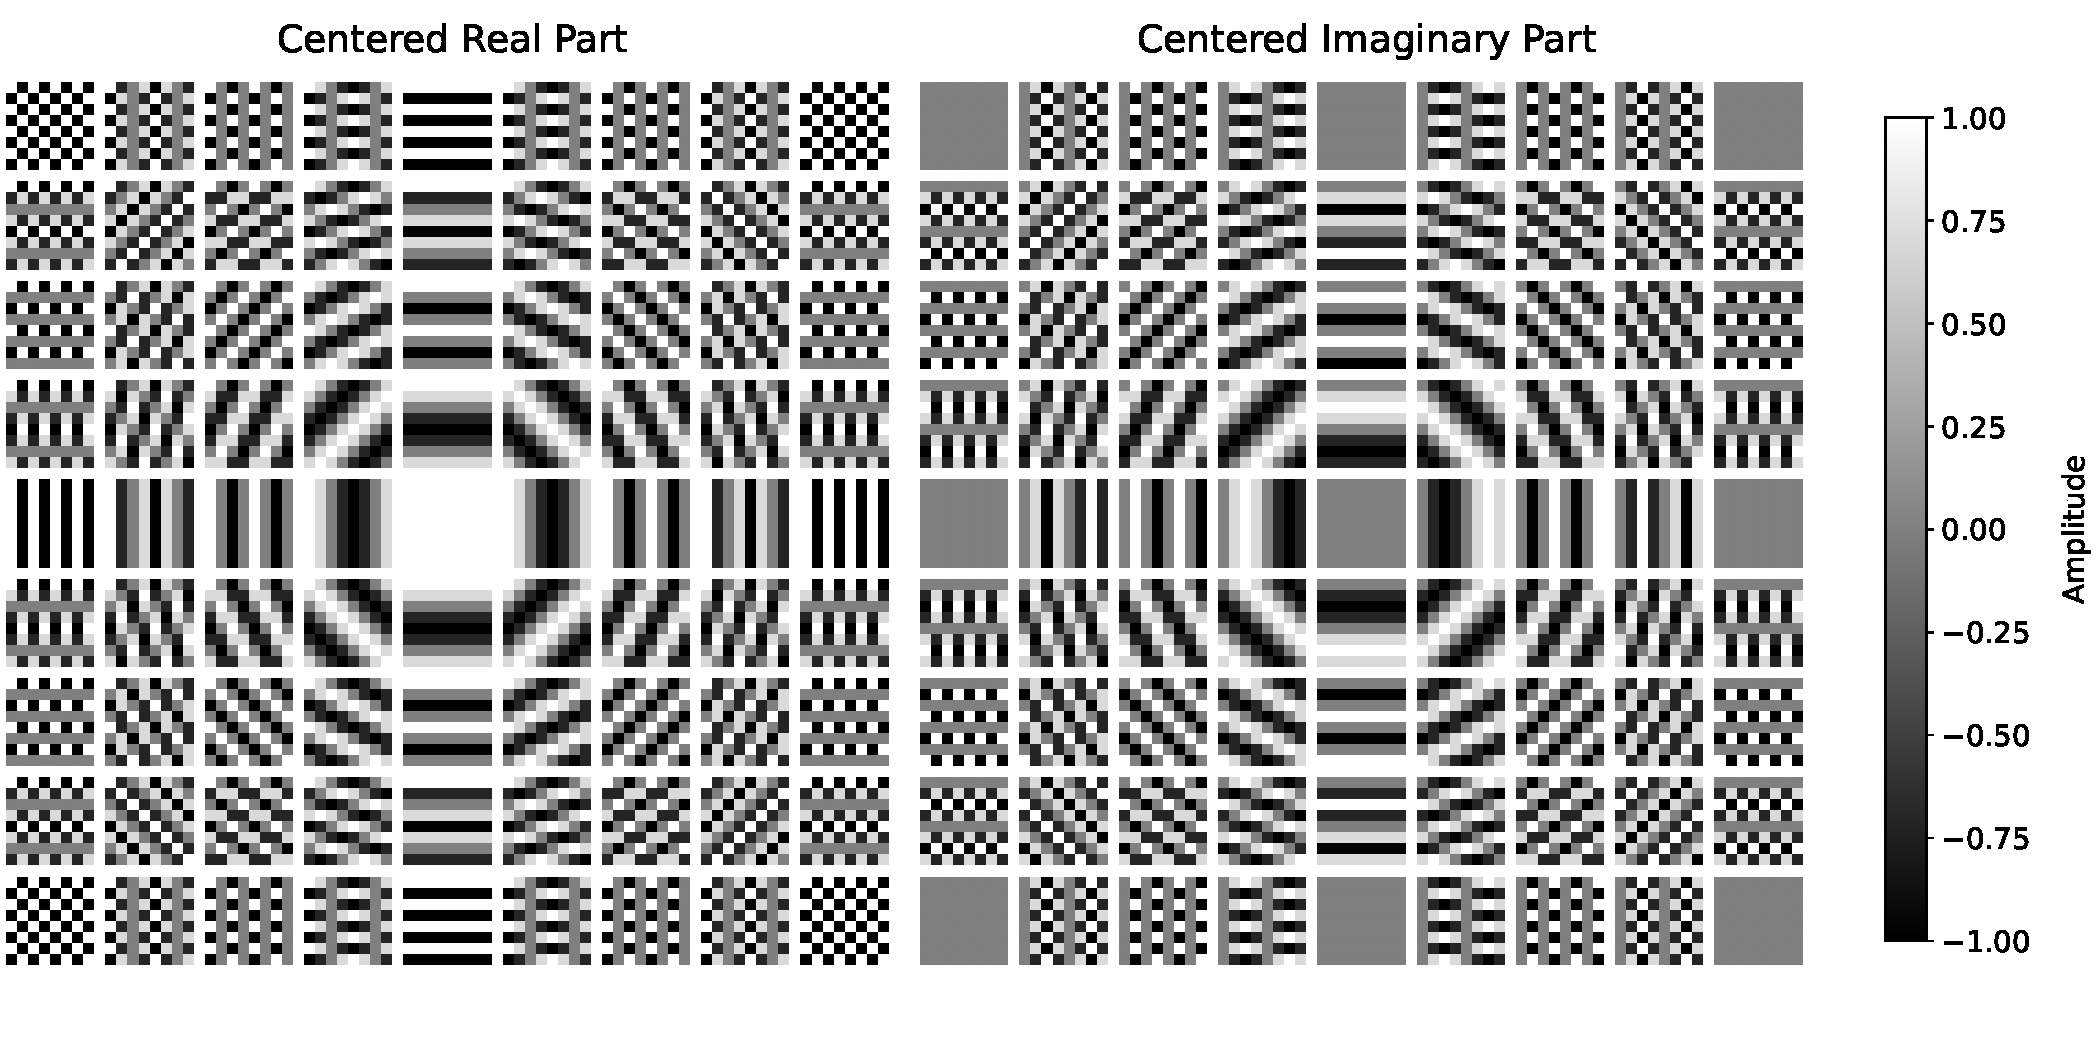
\includegraphics[width=0.95\textwidth]{figures/theory/fourier_basis_2d_en.pdf}
    \caption{Visualization of 2D Fourier basis functions for all frequency pairs $(u,v)$ of an image of size $9 \times 9$. The real and imaginary parts are displayed separately. Low frequencies lie at the center of the grids, while high frequencies lie at the edges.}
    \label{fig:fourier_basis_2d}
\end{figure}

In figures, frequencies are sometimes shown in a centered arrangement, with low frequencies
at the center of the image. This convention is convenient for visualization. In the formulas, however,
the indices always remain in $\{0,\dots,N-1\}$ and are interpreted modulo $N$.

\subsection{Vectorization and the Kronecker Product}

Throughout this chapter, we vectorize images by stacking their columns. For
$X\in\mathbb{C}^{N\times N}$, we therefore define
\begin{equation}
\operatorname{vec}(X)
=
\begin{pmatrix}
X[0,0] \\
X[1,0] \\
\vdots \\
X[N-1,0] \\
X[0,1] \\
\vdots \\
X[N-1,N-1]
\end{pmatrix}.
\label{eq:def_vectorisation_colonnes}
\end{equation}
The first column is read first, then the second, and so on. Under this convention,
entry $X[m,n]$ corresponds to the vectorized index
\[
    m+Nn.
\]

We also use the Kronecker product, denoted by $\otimes$. It is defined as follows: for
$A \in \mathbb{C}^{m \times n}$ and $B \in \mathbb{C}^{p \times q}$, the block matrix of size
$mp \times nq$ is defined by

$$
A \otimes B =
\begin{pmatrix}
a_{11}B & a_{12}B & \cdots & a_{1n}B \\
a_{21}B & a_{22}B & \cdots & a_{2n}B \\
\vdots  & \vdots  & \ddots & \vdots  \\
a_{m1}B & a_{m2}B & \cdots & a_{mn}B
\end{pmatrix}.
$$

In particular, it allows us to construct
a 2D Fourier basis from two 1D Fourier bases. The algebraic properties of
vectorization and the Kronecker product are established results in matrix analysis~\cite{horn2013matrix}.

Under our column-wise vectorization convention, in particular,
\begin{equation}
    \operatorname{vec}(ab^T)
    =
    b\otimes a.
    \label{eq:vec_produit_exterieur}
\end{equation}

Applying this identity to the Fourier image
\[
    \Phi_{u,v}=\phi_u\phi_v^T,
\]
gives
\begin{equation}
    \operatorname{vec}(\Phi_{u,v})
    =
    \phi_v\otimes\phi_u.
    \label{eq:vec_fourier_2d}
\end{equation}
Thus, throughout the remainder of the chapter, the column of $Q_N$ associated with the 2D frequency $(u,v)$ is denoted by
\[
    q_{u,v}
    =
    \phi_v\otimes\phi_u.
\]

We then denote by
\begin{equation}
    Q_N = F_N \otimes F_N
    \label{eq:def_base_fourier_2d_vectorisee}
\end{equation}
the vectorized 2D Fourier basis. Since $F_N$ is unitary,
\[
    Q_N^H Q_N = I_{N^2}.
\]
The columns of $Q_N$ form an orthonormal basis of $\mathbb{C}^{N^2}$.

With the preceding notation, the column associated with frequency $(u,v)$ is
\[
    (Q_N)_{w(u,v)}
    =
    q_{u,v}
    =
    \phi_v\otimes\phi_u.
\]
The index $w(u,v)$ is simply the flattened index that maps the frequency pair
$(u,v)$ to a single column index in $Q_N$. It is defined by
\begin{equation}
    w(u,v)=u+Nv.
    \label{eq:indice_frequence_aplati}
\end{equation}\

Conversely, given a flattened index $w\in\{0,\dots,N^2-1\}$, the corresponding frequency
pair is recovered as
\[
    u = w \bmod N,
    \qquad
    v = \left\lfloor \frac{w}{N} \right\rfloor.
\]

\section{Discrete Convolution in Dimension 1}

Before studying images, we begin with the simpler case of a periodic discrete signal represented
by one period $x = (x[0], x[1], \ldots, x[N-1])$ with $x[i] \in \mathbb{R}$.
Let $x \in \mathbb{R}^N$ be our signal and $h = (h[0], h[1], \ldots, h[N-1]) \in \mathbb{R}^N$ our filter (assumed
to have the same size as the signal, with zero-padding if necessary).
The circular convolution of $h$ and $x$ is defined as

\[
y[n] = (h * x)[n] = \sum_{k=0}^{N-1} h[k]\,x[(n-k) \bmod N] \text{~\cite{ImagerieNumeriqueTheme7Block2}}
\]

The modulo operation means that the signal indices are taken in
\(\mathbb{Z}_N\). 
Thus, when an index falls outside the interval \(\{0,\ldots,N-1\}\),
it is mapped back to its corresponding class in \(\mathbb{Z}_N\).
The signal is therefore interpreted as periodic, as illustrated in
Figure~\ref{fig:padding_circulaire}.

\begin{figure}[H]
    \centering
    \begin{tikzpicture}[
        node distance=0cm,
        cell/.style={rectangle, draw=black, thick, minimum width=1.2cm, minimum height=1.2cm, text centered, font=\large},
        pad/.style={rectangle, draw=gray, dashed, fill=gray!10, minimum width=1.2cm, minimum height=1.2cm, text centered, font=\large, text=gray}
    ]
    
    \node[cell] (x0) {$x_0$};
    \node[cell, right=of x0] (x1) {$x_1$};
    \node[cell, right=of x1] (x2) {$x_2$};
    \node[cell, right=of x2] (x3) {$x_3$};
    
    \node[pad, left=of x0] (pL1) {$x_3$};
    \node[pad, left=of pL1] (pL2) {$x_2$};
    
    \node[pad, right=of x3] (pR1) {$x_0$};
    \node[pad, right=of pR1] (pR2) {$x_1$};
    
    \draw [decorate,decoration={brace,amplitude=5pt,mirror}]
        (x0.south west) -- (x3.south east) node[midway,below=10pt] {Original signal $x$};
    
    \draw [decorate,decoration={brace,amplitude=5pt}, gray]
        (pL2.north west) -- (pL1.north east) node[midway,above=10pt] {\textit{Padding}};
        
    \draw [decorate,decoration={brace,amplitude=5pt}, gray]
        (pR1.north west) -- (pR2.north east) node[midway,above=10pt] {\textit{Padding}};

    \draw[->, thick, gray, dashed, bend left=45] (x3.north) to node[above] {} (pL1.north);
    \draw[->, thick, gray, dashed, bend right=45] (x0.south) to node[below] {} (pR1.south);

    \end{tikzpicture}
    \caption{Circular \textit{padding} for a 1D signal. The signal boundaries repeat periodically.}
    \label{fig:padding_circulaire}
\end{figure}

\paragraph{Remark on the periodicity assumption.}

In this section, we work with circular convolutions. This amounts to treating
signals as periodically extended: when we pass one end of the signal, we continue
from the other end. This assumption is mathematically useful because it allows
convolutions to be diagonalized by the discrete Fourier basis.

However, it does not always match the exact boundary behavior of real images:
if the ends do not join naturally, periodization can create an artificial
discontinuity. This point is discussed in greater detail in Appendix~\ref{app:periodicite-bords-gibbs}.

\section{Fourier Functions as Eigenfunctions of Circular Convolution}
\label{sec:fourier-vecteurs-propres}

\paragraph{One-dimensional case.}

We work in the space of periodic discrete signals with period $N$:
\[
V_N = \{x : \mathbb{Z}_N \rightarrow \mathbb{C}\}.
\]
An element of $V_N$ can be viewed either as a periodic discrete function or as a vector in $\mathbb{C}^N$.

For a fixed filter $h \in \mathbb{C}^N$, circular convolution defines a linear operator
\[
\mathcal{C}_h : V_N \rightarrow V_N,
\qquad
\mathcal{C}_h(x) = h * x.
\]

For each frequency $f \in \{0,\dots,N-1\}$, we use the normalized Fourier vector
$\phi_f$ defined in \eqref{eq:def_base_fourier_1d}.

The fundamental result connecting circular convolution and the Fourier basis is then

\begin{equation}
\mathcal{C}_h(\phi_f) = \lambda_f \phi_f,
\label{eq:fourier_fonction_propre_conv_1d}
\end{equation}

or, component by component,
\[
(h * \phi_f)[n] = \lambda_f \phi_f[n],
\]
where
\[
\lambda_f =
\sum_{k=0}^{N-1} h[k] e^{-2\mathrm{i}\pi f k/N}.
\]

Note that $\lambda_f$ depends on the filter $h$ and the frequency $f$,
but not on the position $n$. Thus, when the input to the circular convolution operator
is a Fourier mode, convolution does not alter its spatial form: it simply
multiplies it by a complex scalar. In other words, $\lambda_f$ is an eigenvalue and
$\phi_f$ an eigenfunction of the circular convolution operator
$\mathcal{C}_h$.

\begin{proof}
\begin{alignat*}{2}
    (\mathcal{C}_h(\phi_f))[n] &= (h * \phi_f)[n] \\
    &= \sum_{k=0}^{N-1} h[k]\,\phi_f[(n-k) \bmod N] \\
    \text{\small (periodicity of $\phi_f$)} \quad &= \sum_{k=0}^{N-1} h[k]\,\phi_f[n-k] \\
    \text{\small (property of exponentials)} \quad &= \sum_{k=0}^{N-1} h[k] e^{-2\mathrm{i}\pi f k/N}\phi_f[n] \\
    &= \left(\sum_{k=0}^{N-1} h[k] e^{-2\mathrm{i}\pi f k/N}\right)\phi_f[n] \\
    &= \lambda_f \phi_f[n].
\end{alignat*}

\end{proof}

This result corresponds to the discrete convolution theorem: in the Fourier domain,
circular convolution becomes frequency-wise multiplication. Thus,
when the input is a pure Fourier mode \(\phi_f\), convolution does not change
its frequency; it only multiplies it by a scalar. We therefore obtain Equation~\ref{eq:fourier_fonction_propre_conv_1d}.

\subsection{Consequence: Diagonalization of Circulant Matrices}

For a fixed filter $h$, 1D circular convolution defines a linear map $\mathbb{C}^N \rightarrow \mathbb{C}^N$,
since for all $x, y \in \mathbb{C}^N$ and all $\alpha, \beta \in \mathbb{C}$,
\begin{align*}
h * (\alpha x + \beta y) &= \alpha (h * x) + \beta (h * y)
\end{align*}

\begin{proof}
\begin{alignat*}{2}
    (h * (\alpha x + \beta y))[n] &= \sum_{k=0}^{N-1} h[k]\,(\alpha x + \beta y)[(n-k) \bmod N]  \\
    &= \sum_{k=0}^{N-1} h[k]\,(\alpha x[(n-k) \bmod N] + \beta y[(n-k) \bmod N])  \\
    &= \alpha \sum_{k=0}^{N-1} h[k]\,x[(n-k) \bmod N] + \beta \sum_{k=0}^{N-1} h[k]\,y[(n-k) \bmod N]  \\
    &= \alpha (h * x)[n] + \beta (h * y)[n].
\end{alignat*}

\end{proof}

Since this operation is linear, the result reviewed in Appendix~\ref{app:representation-lineaire-matrice}
guarantees that, once a basis has been chosen, it can be represented by a matrix
$C_h \in \mathbb{C}^{N \times N}$ such that, for every input signal $x \in \mathbb{C}^N$,

$$
y = C_h x.
$$

Here, $C_h$ is a circulant matrix constructed from the filter $h$. Its first row is arranged to reproduce $y[0]$,
and each subsequent row is obtained by a circular shift:

$$
C_h =
\begin{pmatrix}
h[0] & h[N-1] & h[N-2] & \cdots & h[1] \\
h[1] & h[0] & h[N-1] & \cdots & h[2] \\
h[2] & h[1] & h[0] & \cdots & h[3] \\
\vdots & \vdots & \vdots & \ddots & \vdots \\
h[N-1] & h[N-2] & h[N-3] & \cdots & h[0]
\end{pmatrix}.
$$

Indeed, $y[0] = h[0]x[0] + h[1]x[N-1] + \cdots + h[N-1]x[1]$ is the first row of $C_h$
multiplied by the vector $x$. Applying the same reasoning iteratively gives the other elements of $y$.

\vspace{0.5cm}

In the standard basis of $\mathbb{C}^N$, the linear operator $\mathcal{C}_h$
is represented by the circulant matrix $C_h$. The relation
$\mathcal{C}_h(\phi_f) = \lambda_f \phi_f$ can then be rewritten in matrix form:

\begin{equation}
    C_h \phi_f = \lambda_f \phi_f
    \label{eq:fourier_eigen_matrice}
\end{equation}

Thus, each Fourier function $\phi_f$ is an eigenvector of the circulant matrix $C_h$,
with associated eigenvalue $\lambda_f$. This means that, in the circular
setting, convolution acts diagonally in the Fourier basis.

Using the Fourier matrix $F_N$ defined in \eqref{eq:def_matrice_fourier_1d},
we collect the eigenvalues in the diagonal matrix
$$
\Lambda_h =
\operatorname{diag}(\lambda_0,\lambda_1,\ldots,\lambda_{N-1}).
$$

Combining the vector equalities \eqref{eq:fourier_eigen_matrice} for all frequencies gives

\begin{align}
C_h F_N &= F_N \Lambda_h \notag \\
\text{(by unitarity of \(F_N\))}\qquad
\Longleftrightarrow\quad
C_h &= F_N \Lambda_h F_N^H.
\end{align}

\section{Circular Convolution in Dimension 2}
\label{sec:convolution-circulaire-2d}

We now extend the preceding result to square images. Let
$X\in\mathbb{C}^{N\times N}$ be an image and
$h\in\mathbb{C}^{N\times N}$ a filter. 2D circular convolution is defined by
\begin{equation}
    Y[m,n]
    =
    (h * X)[m,n]
    =
    \sum_{a=0}^{N-1}
    \sum_{b=0}^{N-1}
    h[a,b]\,
    X[(m-a)\bmod N,\,(n-b)\bmod N].
    \label{eq:def_convolution_circulaire_2d}
\end{equation}

We use the 2D Fourier images defined in \eqref{eq:def_base_fourier_2d}:
\[
    \Phi_{u,v}[m,n]
    =
    \phi_u[m]\phi_v[n].
\]
As in dimension 1, a circular shift of a Fourier basis function does not change its form, but
multiplies it by a complex factor:
\[
    \phi_u[(m-a)\bmod N]
    =
    e^{-2\pi iua/N}\phi_u[m],
    \qquad
    \phi_v[(n-b)\bmod N]
    =
    e^{-2\pi ivb/N}\phi_v[n].
\]
Thus,
\[
    \Phi_{u,v}[(m-a)\bmod N,(n-b)\bmod N]
    =
    e^{-2\pi i(ua+vb)/N}
    \Phi_{u,v}[m,n],
\]

where $(ua + vb) \in \mathbb{Z}_N$.

Applying 2D circular convolution to $\Phi_{u,v}$ gives
\begin{align}
(h * \Phi_{u,v})[m,n]
&=
\sum_{a=0}^{N-1}
\sum_{b=0}^{N-1}
h[a,b]\,
\Phi_{u,v}[(m-a)\bmod N,(n-b)\bmod N]
\nonumber \\
&=
\left(
\sum_{a=0}^{N-1}
\sum_{b=0}^{N-1}
h[a,b]e^{-2\pi i(ua+vb)/N}
\right)
\Phi_{u,v}[m,n].
\end{align}

We therefore define
\begin{equation}
    \lambda_{u,v}
    =
    \sum_{a=0}^{N-1}
    \sum_{b=0}^{N-1}
    h[a,b]e^{-2\pi i(ua+vb)/N}.
    \label{eq:valeur_propre_convolution_2d}
\end{equation}
Finally, we obtain
\begin{equation}
    h * \Phi_{u,v}
    =
    \lambda_{u,v}\Phi_{u,v}.
    \label{eq:fourier_fonction_propre_conv_2d}
\end{equation}

\section{Matrix Representation of a 2D Convolution}

We now use the column-wise vectorization defined in
\eqref{eq:def_vectorisation_colonnes}. Since circular convolution is linear, there exists
a matrix
\[
    M \in \mathbb{C}^{N^2\times N^2}
\]
such that
\begin{equation}
    \operatorname{vec}(Y)
    =
    M\operatorname{vec}(X).
\end{equation}

In other words, the coefficient of $M$ at row $m+Nn$ and column $r+Ns$ indicates how pixel
$X[r,s]$ contributes to pixel $Y[m,n]$.

The matrix $M$ applies the filter $h$ to every pixel of our image $X$ in a single operation.
To do so, $M$ has a block-circulant structure with circulant blocks (BCCB),
as illustrated below:

\begin{figure}[H]
\centering

\begin{tikzpicture}[
    scale=0.75, transform shape, % Réduction globale équilibrée
    font=\small,
    block/.style={
        draw=black!65,
        rounded corners=1pt,
        minimum width=1.0cm,  % Réduit de 1.25
        minimum height=0.55cm, % Réduit de 0.70
        inner sep=1pt,
        fill=gray!6,
        align=center
    },
    diagblock/.style={
        block,
        fill=gray!18,
        draw=black!85,
        line width=0.5pt
    },
    frame/.style={
        draw=black!85,
        rounded corners=2pt,
        line width=0.6pt
    },
    arrow/.style={
        -{Stealth[length=1.5mm]},
        semithick,
        black!65
    }
]

% --- Matrice M (plus compacte) ---
\matrix (B) [
    matrix of nodes,
    nodes={block},
    row sep=1.5pt,    % Espacement réduit
    column sep=1.5pt  % Espacement réduit
] {
|[diagblock]|$C_0$     & $C_{N-1}$ & $\cdots$ & $C_2$     & $C_1$     \\
$C_1$                 & |[diagblock]|$C_0$ & $\cdots$ & $C_3$     & $C_2$     \\
$\vdots$              & $\vdots$   & $\ddots$ & $\vdots$  & $\vdots$  \\
$C_{N-2}$             & $C_{N-3}$  & $\cdots$ & |[diagblock]|$C_0$ & $C_{N-1}$ \\
$C_{N-1}$             & $C_{N-2}$  & $\cdots$ & $C_1$     & |[diagblock]|$C_0$ \\
};

\node[frame, fit=(B-1-1)(B-5-5), inner sep=3pt] (bigmatrix) {};

% Titre compact avec sous-titre intégré
\node[above=2pt of bigmatrix, align=center] {
    \textbf{\(M \in\mathbb{C}^{N^2\times N^2}\)} \\ 
    \scriptsize (Block-circulant: shifts of blocks)
};

% --- Flèche de zoom plus courte ---
\draw[arrow] (bigmatrix.east) -- ++(0.7,0) node[midway, above, font=\tiny] {zoom};

% --- Bloc Ck (Matrice resserrée) ---
\node[anchor=west] (circulant) at ($(bigmatrix.east)+(0.9cm,0)$) {$\displaystyle
C_k =
\begin{bmatrix}
h_{0,k}     & \cdots & h_{1,k} \\
h_{1,k}     & \cdots & h_{2,k} \\
\vdots      & \ddots & \vdots  \\
h_{N-1,k}   & \cdots & h_{0,k}
\end{bmatrix}
$};

\node[frame, fit=(circulant), inner sep=2pt] (smallmatrix) {};

% Titre compact pour Ck
\node[above=2pt of smallmatrix, align=center] {
    \textbf{Circulant block \(C_k\)} \\
    \scriptsize (internal shifts)
};

\end{tikzpicture}

\caption{Compact structure of a BCCB (doubly circulant) matrix.}
\label{fig:bccb-structure}
\end{figure}

We therefore call $M$ a \textbf{BCCB} matrix (\textit{Block-Circulant with Circulant Blocks}~\cite{jain1989fundamentals}).
Details are provided in Appendix~\ref{app:preuve_bccb}.

The spectral result obtained for 2D circular convolution then becomes, in vectorized form,
\[
    M\operatorname{vec}(\Phi_{u,v})
    =
    \lambda_{u,v}\operatorname{vec}(\Phi_{u,v}).
\]

\subsection{Diagonalization by the Kronecker Product of Fourier Bases}

From the preceding result \ref{eq:fourier_fonction_propre_conv_2d}, since \(q_{u,v}=\operatorname{vec}(\Phi_{u,v})\), we obtain
\[
    M q_{u,v}
    =
    \lambda_{u,v} q_{u,v}.
\]
Combining the equalities for all frequencies gives the matrix identity
\begin{equation}
    \begin{split}
        M Q_N &= Q_N \Lambda_h \\
        \Longleftrightarrow \text{\footnotesize (unitarity of $Q_N$)} \quad M &= Q_N \Lambda_h Q_N^H.
    \end{split}
    \label{eq:diagonalisation_conv_2d}
\end{equation}
Here, $\Lambda_h$ is the diagonal matrix containing the eigenvalues $\lambda_{u,v}$
in the same order as the columns $q_{u,v}$ of $Q_N$.

\section{Extension to the Multichannel Case}

So far, we have considered single-channel convolution, where the input
and output images each have a single channel (for example, a grayscale image).
We now consider the more general case of multichannel convolution:
\[
    X \in\mathbb{C}^{m_{in} \times N \times N}, \qquad Y \in\mathbb{C}^{m_{out} \times N \times N},
\]
where $m_{in}$ and $m_{out}$ denote the number of input and output channels, respectively.

For each output channel $Y_i$,
\begin{equation}
    Y_i = \sum_{j=1}^{m_{in}} h_{i,j} * X_j \qquad\text{for } i=1,\dots,m_{out},
    \label{eq:conv_multi}
\end{equation}
where $h_{i,j}$ is the convolution filter applied to input channel $j$ to produce output channel $i$.

% \begin{figure}[H]
%     \centering
%     % J'ai baissé très légèrement le scale à 0.85 pour que ce schéma plus large rentre 
%     % parfaitement dans les marges classiques d'un document A4.
%     \begin{tikzpicture}[>=stealth, font=\sffamily, scale=0.85, every node/.style={transform shape}]
        
%         % ==========================================
%         % Couleurs
%         % ==========================================
%         \definecolor{gridblue}{HTML}{006699}
%         \definecolor{gridred}{HTML}{E74C3C}
%         \definecolor{gridteal}{HTML}{148F77}
%         \definecolor{gridorange}{HTML}{F39C12}
%         \definecolor{bglight}{HTML}{F8F9FA}

%         % ==========================================
%         % Zones de fond (Structuration élargie)
%         % ==========================================
%         \draw[fill=bglight, draw=gray!40, dashed, rounded corners=5pt] 
%             (-1.0, -1.0) rectangle (1.0, 6.0);
%         \node[gray, font=\bfseries\small] at (0, 5.65) {Entrée $X$};

%         \draw[fill=bglight, draw=gray!40, dashed, rounded corners=5pt] 
%             (3.0, -1.0) rectangle (5.0, 6.0);
%         \node[gray, font=\bfseries\small, align=center] at (4.0, 5.65) {Filtres $h_i$};

%         \draw[fill=bglight, draw=gray!40, dashed, rounded corners=5pt] 
%             (7.0, -1.0) rectangle (9.0, 6.0);
%         \node[gray, font=\bfseries\small, align=center] at (8.0, 5.65) {Cartes $Z_i$};

%         \draw[fill=bglight, draw=gray!40, dashed, rounded corners=5pt] 
%             (10.8, -1.0) rectangle (15.5, 6.0);
%         \node[gray, font=\bfseries\small, align=center] at (13.15, 5.65) {Somme et Sortie};

%         % ==========================================
%         % 1. Canal Supérieur (m_in)
%         % ==========================================
%         % X_min (Centre x=0, y=3.8)
%         \filldraw[fill=gridblue!10, draw=gridblue, thick] 
%             (-0.625, 3.175) rectangle ++(1.25,1.25);
%         \draw[gridblue!40, step=0.3125] (-0.625, 3.175) grid ++(1.25,1.25);
%         \node[gridblue, font=\bfseries\scriptsize, fill=white, fill opacity=0.8, text opacity=1, inner sep=1.5pt] 
%             at (0, 3.8) {$X_{m_{\mathrm{in}}}$};

%         % Conv node * (Centre x=4.0, y=3.8)
%         \node[circle, draw=gridorange, fill=gridorange!10, thick, minimum size=0.5cm, inner sep=0pt] 
%             (convtop) at (4.0, 3.8) {$*$};

%         % h_min (Centre x=4.0, y=5.0)
%         \filldraw[fill=gridred!10, draw=gridred, thick] 
%             (3.575, 4.575) rectangle ++(0.85,0.85);
%         \draw[gridred!45, step=0.2125] (3.575, 4.575) grid ++(0.85,0.85);
%         \node[gridred, font=\bfseries\scriptsize, fill=white, fill opacity=0.8, text opacity=1, inner sep=1.5pt] 
%             at (4.0, 5.0) {$h_{i,m_{\mathrm{in}}}$};

%         % Z_min (Centre x=8.0, y=3.8)
%         \filldraw[fill=gridorange!15, draw=gridorange, thick] 
%             (7.45, 3.25) rectangle ++(1.10,1.10);
%         \draw[gridorange!45, step=0.275] (7.45, 3.25) grid ++(1.10,1.10);
%         \node[gridorange!80!black, font=\bfseries\scriptsize, fill=white, fill opacity=0.8, text opacity=1, inner sep=1.5pt] 
%             at (8.0, 3.8) {$Z_{i,m_{\mathrm{in}}}$};

%         % Flèches Canal m_in
%         \draw[->, thick, gridblue] (0.625, 3.8) -- (convtop.west);
%         \draw[->, thick, gridred] (4.0, 4.575) -- (convtop.north);
%         \draw[->, thick, gridorange] (convtop.east) -- (7.45, 3.8);

%         % ==========================================
%         % 2. Canal Inférieur (1)
%         % ==========================================
%         % X_1 (Centre x=0, y=0)
%         \filldraw[fill=gridblue!25, draw=gridblue, thick] 
%             (-0.625, -0.625) rectangle ++(1.25,1.25);
%         \draw[gridblue!45, step=0.3125] (-0.625, -0.625) grid ++(1.25,1.25);
%         \node[gridblue, font=\bfseries\scriptsize, fill=white, fill opacity=0.85, text opacity=1, inner sep=2pt] 
%             at (0, 0) {$X_1$};

%         % Conv node * (Centre x=4.0, y=0)
%         \node[circle, draw=gridorange, fill=gridorange!10, thick, minimum size=0.5cm, inner sep=0pt] 
%             (convbot) at (4.0, 0) {$*$};

%         % h_1 (Centre x=4.0, y=1.2)
%         \filldraw[fill=gridred!25, draw=gridred, thick] 
%             (3.575, 0.775) rectangle ++(0.85,0.85);
%         \draw[gridred!45, step=0.2125] (3.575, 0.775) grid ++(0.85,0.85);
%         \node[gridred, font=\bfseries\scriptsize, fill=white, fill opacity=0.85, text opacity=1, inner sep=2pt] 
%             at (4.0, 1.2) {$h_{i,1}$};

%         % Z_1 (Centre x=8.0, y=0)
%         \filldraw[fill=gridorange!25, draw=gridorange, thick] 
%             (7.45, -0.55) rectangle ++(1.10,1.10);
%         \draw[gridorange!45, step=0.275] (7.45, -0.55) grid ++(1.10,1.10);
%         \node[gridorange!80!black, font=\bfseries\scriptsize, fill=white, fill opacity=0.85, text opacity=1, inner sep=2pt] 
%             at (8.0, 0) {$Z_{i,1}$};

%         % Flèches Canal 1
%         \draw[->, thick, gridblue] (0.625, 0) -- (convbot.west);
%         \draw[->, thick, gridred] (4.0, 0.775) -- (convbot.north);
%         \draw[->, thick, gridorange] (convbot.east) -- (7.45, 0);

%         % ==========================================
%         % 3. Intermédiaires (Points de suspension)
%         % ==========================================
%         \node[gridblue, font=\Large] at (0, 1.9) {$\vdots$};
%         \node[gridorange, font=\Large] at (4.0, 1.9) {$\vdots$}; 
%         \node[gridorange!80!black, font=\Large] at (8.0, 1.9) {$\vdots$};

%         % ==========================================
%         % 4. Somme & Sortie
%         % ==========================================
%         % Sum (Centre x=12.0)
%         \node[circle, draw=gridteal, fill=gridteal!10, thick, minimum size=0.85cm] 
%             (sum) at (12.0, 1.9) {\Large $\sum$};
%         \node[gridteal, font=\scriptsize, align=center] at (12.0, 1.1) {somme\\sur $j$};

%         % Flèches Z -> Somme
%         \draw[->, thick, gridorange] (8.55, 3.8) to[out=0,in=135] (sum.north west);
%         \draw[->, thick, gridorange] (8.55, 0) to[out=0,in=225] (sum.south west);

%         % Y_i (Centre x=14.2)
%         \filldraw[fill=gridteal!22, draw=gridteal, thick] 
%             (13.525, 1.225) rectangle ++(1.35,1.35);
%         \draw[gridteal!45, step=0.3375] (13.525, 1.225) grid ++(1.35,1.35);
%         \node[gridteal, font=\bfseries\scriptsize, fill=white, fill opacity=0.85, text opacity=1, inner sep=2pt] 
%             at (14.2, 1.9) {$Y_i$};

%         % Flèche Somme -> Y_i
%         \draw[->, thick, gridteal] (sum.east) -- (13.525, 1.9);

%         % ==========================================
%         % 5. Equations Mathématiques (En bas, aérées)
%         % ==========================================
%         \node[gridblue, font=\bfseries\small] at (0, -1.8) {$X \in \mathbb{C}^{m_{\mathrm{in}}\times N\times N}$};
%         \node[gridred, font=\bfseries\small] at (4.0, -1.8) {$h_i \in \mathbb{C}^{m_{\mathrm{in}}\times k\times k}$};
%         \node[gridorange!80!black, font=\bfseries\small] at (8.0, -1.8) {$Z_{i,j}=h_{i,j} * X_j$};
%         \node[gridteal, font=\bfseries\small] at (13.15, -1.8) {$Y_i=\displaystyle\sum_{j=1}^{m_{\mathrm{in}}} Z_{i,j}$};

%     \end{tikzpicture}

%     \vspace{0.3cm}
%     \caption{
%     Convolution multi-canaux produisant un canal de sortie $Y_i$.
%     }
%     \label{fig:conv_multi_canaux}
% \end{figure}

\subsection{Channel Mixing at a Fixed Frequency}
\label{subsec:melange_canaux_frequence_fixee}

Consider a spatial frequency $(u,v)$ and the corresponding Fourier image $\Phi_{u,v}$.
Assume that each input channel contains this same spatial frequency, but with a different
amplitude:
\[
    X_j = \alpha_j \Phi_{u,v},
    \qquad j=1,\dots,m_{\mathrm{in}}.
\]
The vector
\[
    \alpha = (\alpha_1,\dots,\alpha_{m_{\mathrm{in}}})^T
\]
therefore contains the amplitudes of this frequency in the different input channels.

Substituting these inputs into \eqref{eq:conv_multi} and using linearity of convolution gives, for output channel $i$,
\begin{align*}
Y_i
&=
\sum_{j=1}^{m_{\mathrm{in}}} h_{i,j} * X_j \\
&=
\sum_{j=1}^{m_{\mathrm{in}}} \alpha_j (h_{i,j} * \Phi_{u,v}) \\
&=
\sum_{j=1}^{m_{\mathrm{in}}} \alpha_j \lambda^{i,j}_{u,v}\Phi_{u,v} \\
&=
\left(
    \sum_{j=1}^{m_{\mathrm{in}}}
    \lambda^{i,j}_{u,v}\alpha_j
\right)
\Phi_{u,v}.
\end{align*}

We then introduce the mixing matrix associated with frequency $(u,v)$:
\[
    G^{(u,v)} \in \mathbb{C}^{m_{\mathrm{out}}\times m_{\mathrm{in}}},
    \qquad
    G^{(u,v)}_{i,j}
    =
    \lambda^{i,j}_{u,v}.
\]
If $\beta\in\mathbb{C}^{m_{\mathrm{out}}}$ denotes the output amplitudes of this same frequency,
we can simply write
\[
    \beta = G^{(u,v)}\alpha.
\]

This expression summarizes the role of multichannel convolution: for a fixed spatial frequency,
it performs linear mixing across channels.

\subsection{Global Matrix Form}

To express the multichannel operation in global matrix form, we define
\[
\mathbf{x}
=
\begin{pmatrix}
\operatorname{vec}(X_1) \\
\vdots \\
\operatorname{vec}(X_{m_{\mathrm{in}}})
\end{pmatrix}
\in \mathbb{C}^{m_{\mathrm{in}}N^2},
\qquad
\mathbf{y}
=
\begin{pmatrix}
\operatorname{vec}(Y_1) \\
\vdots \\
\operatorname{vec}(Y_{m_{\mathrm{out}}})
\end{pmatrix}
\in \mathbb{C}^{m_{\mathrm{out}}N^2}.
\]

For each channel pair $(i,j)$, let $B^{i,j}$ denote the spatial convolution matrix
associated with filter $h_{i,j}$, that is, the matrix applying convolution between input
channel $j$ and output channel $i$.
We use the vectorized 2D Fourier basis $Q_N$ defined in
\eqref{eq:def_base_fourier_2d_vectorisee}. For each channel pair $(i,j)$, the matrix
$B^{i,j}$ can therefore be diagonalized as
\[
    B^{i,j}
    =
    Q_N D^{i,j} Q_N^H,
\]
where
\[
D^{i,j}
=
\operatorname{diag}\bigl(
\lambda^{i,j}_{u,v}
\bigr)_{(u,v)\in\{0,\dots,N-1\}^2}.
\]

The diagonal entries of $D^{i,j}$ are ordered according to the flattened index
$w(u,v)$ defined in \eqref{eq:indice_frequence_aplati}.

We can now introduce the global matrix $M \in \mathbb{C}^{m_{out}N^2 \times m_{in}N^2}$,
which represents the entire convolutional layer as a block matrix of size
$m_{out} \times m_{in}$, where each block $(i,j)$ corresponds to the application of filter $h_{i,j}$:

$$
M =
\begin{pmatrix}
B^{1,1} & \cdots & B^{1,m_{in}} \\
\vdots & \ddots & \vdots \\
B^{m_{out},1} & \cdots & B^{m_{out},m_{in}}
\end{pmatrix}.
$$

Since the same basis $Q_N$ diagonalizes all spatial blocks $B^{i,j}$, we can factor out the spatial
change of basis on either side of the block matrix. This gives

\begin{equation}
    M = (I_{m_{out}} \otimes Q_N) L (I_{m_{in}} \otimes Q_N)^H
    \label{eq:factorisation_M}
\end{equation}

where $L \in \mathbb{C}^{m_{out}N^2 \times m_{in}N^2}$ is a block matrix with diagonal blocks:

$$
L =
\begin{pmatrix}
D^{1,1} & \cdots & D^{1,m_{in}} \\
\vdots & \ddots & \vdots \\
D^{m_{out},1} & \cdots & D^{m_{out},m_{in}}
\end{pmatrix}.
$$

\vspace{0.5cm}
\begin{proof}

By the definition of the Kronecker product, the operations
$I_{m_{out}} \otimes Q_N$ and $(I_{m_{in}} \otimes Q_N)^H = I_{m_{in}} \otimes Q_N^H$
generate block-diagonal matrices:

$$
I_{m_{out}} \otimes Q_N = 
\begin{pmatrix}
Q_N & 0 & \cdots & 0 \\
0 & Q_N & \cdots & 0 \\
\vdots & \vdots & \ddots & \vdots \\
0 & 0 & \cdots & Q_N
\end{pmatrix},
\quad
I_{m_{in}} \otimes Q_N^H = 
\begin{pmatrix}
Q_N^H & 0 & \cdots & 0 \\
0 & Q_N^H & \cdots & 0 \\
\vdots & \vdots & \ddots & \vdots \\
0 & 0 & \cdots & Q_N^H
\end{pmatrix}.
$$

Evaluating the block matrix product on the left applies $Q_N$ to each block in the
corresponding rows of $L$:

$$
(I_{m_{out}} \otimes Q_N) L = 
\begin{pmatrix}
Q_N D^{1,1} & \cdots & Q_N D^{1,m_{in}} \\
\vdots & \ddots & \vdots \\
Q_N D^{m_{out},1} & \cdots & Q_N D^{m_{out},m_{in}}
\end{pmatrix}.
$$

Multiplying this result on the right by the second block-diagonal matrix
applies $Q_N^H$ to each block in the corresponding columns:

$$
(I_{m_{out}} \otimes Q_N) L (I_{m_{in}} \otimes Q_N)^H = 
\begin{pmatrix}
Q_N D^{1,1} Q_N^H & \cdots & Q_N D^{1,m_{in}} Q_N^H \\
\vdots & \ddots & \vdots \\
Q_N D^{m_{out},1} Q_N^H & \cdots & Q_N D^{m_{out},m_{in}} Q_N^H
\end{pmatrix}.
$$

Since the single-channel convolution decomposition gives $B^{i,j} = Q_N D^{i,j} Q_N^H$ for
every pair $(i,j)$, we obtain

$$
(I_{m_{out}} \otimes Q_N) L (I_{m_{in}} \otimes Q_N)^H = 
\begin{pmatrix}
B^{1,1} & \cdots & B^{1,m_{in}} \\
\vdots & \ddots & \vdots \\
B^{m_{out},1} & \cdots & B^{m_{out},m_{in}}
\end{pmatrix}
= M.
$$
\end{proof}

This recovers the form of \textbf{Proposition 1} in the paper by Tsuzuku and Sato~\cite{tsuzuku2019structural}.
It separates two phenomena:
\begin{itemize}
    \item the matrices $(I\otimes Q_N)$ perform the spatial change of basis to the Fourier domain;
    \item the central matrix $L$ contains the channel mixing, organized frequency by frequency.
\end{itemize}

\section{Linear Stacking of Convolutions}
\label{sec:empilement-lineaire-convolutions}

We now introduce the notion of stacked convolutional layers.
The aim is to mathematically model the operation of a deep convolutional neural network, which
consists of several layers applied successively.

As shown in the preceding sections, our linear framework allows us to represent each convolutional
layer with stride \(1\) (stride denotes the step size; see \ref{fig:stride_comparison} for an illustration) by a large global matrix \(M^{(k)}\).
Let \(m_k\) denote the number of input channels of layer \(k\), and \(m_{k+1}\) the number of output channels:
\[
M^{(k)} : \mathbb{C}^{m_k N^2} \longrightarrow \mathbb{C}^{m_{k+1}N^2}.
\]

Thus, for a vectorized input \(X \in \mathbb{C}^{m_1N^2}\), the output of the
first layer is
$$
X_1 = M^{(1)} X \in \mathbb{C}^{m_2 N^2}.
$$
Applying a second convolutional layer gives
$$
X_2 = M^{(2)} X_1 = M^{(2)}(M^{(1)} X) = (M^{(2)} M^{(1)}) X.
$$
Continuing in this way for $d$ successive convolutional layers gives
\begin{equation}
M(X) = \left(M^{(d)} M^{(d-1)} \cdots M^{(1)}\right)X.
\label{eq:composition_couches}
\end{equation}

\subsection{Simplification by Telescoping Transformations}

The main advantage of the matrix decomposition in Equation~\eqref{eq:factorisation_M} lies
in its behavior when several layers are multiplied. Consider two successive
layers $M^{(1)}$ and $M^{(2)}$. Their product is
\begin{align*}
M^{(2)}M^{(1)} &= \left[ (I_{m_3} \otimes Q_N) L^{(2)} (I_{m_2} \otimes Q_N)^H \right] \left[ (I_{m_2} \otimes Q_N) L^{(1)} (I_{m_1} \otimes Q_N)^H \right] \\
&= (I_{m_3} \otimes Q_N) L^{(2)} \underbrace{\left( (I_{m_2} \otimes Q_N)^H (I_{m_2} \otimes Q_N) \right)}_{I_{m_2 N^2}} L^{(1)} (I_{m_1} \otimes Q_N)^H
\end{align*}

By induction, for a network of $d$ layers, the global matrix $M$ simplifies to
\[
M = (I_{m_{d+1}} \otimes Q_N) L (I_{m_1} \otimes Q_N)^H
\]
where $L = L^{(d)} L^{(d-1)} \cdots L^{(1)}$ represents the accumulated channel mixing.

\subsection{Frequency Independence and the Mixing Matrix $G^{(w)}$}

Since each internal block of the matrices $L^{(k)}$ is diagonal, their product preserves this structure.
Indeed, block $(i,j)$ of the product of two block matrices $L^{(2)}L^{(1)}$ is
\[
(L^{(2)}L^{(1)})_{i,j}
=
\sum_k D^{(2)}_{i,k}D^{(1)}_{k,j}.
\] 
The product of two diagonal matrices is diagonal, and a sum of diagonal matrices remains diagonal.
Consequently, each block of the global matrix $L = L^{(d)}L^{(d-1)}\cdots L^{(1)}$ is still a diagonal matrix of size $N^2 \times N^2$.

Thus, in a linear stack of circular convolutions with stride $1$, the frequency-wise structure
is preserved. For a given frequency, only the distribution across channels changes.

The idea is therefore as follows: to study what the network does at a given frequency, we do not
need to examine the entire large matrix $L$. It is sufficient to look within each block
$D^{(i,j)}$.

We collect these coefficients in a small matrix
\[
    G^{(w)} \in \mathbb{C}^{m_{\mathrm{out}}\times m_{\mathrm{in}}},
\]
defined by
\begin{equation}
    \bigl(G^{(w)}\bigr)_{i,j}
    =
    \bigl(D^{(i,j)}\bigr)_{w,w}.
    \label{eq:def_matrice_frequence}
\end{equation}

The matrix $G^{(w)}$ therefore describes the network's behavior at frequency $w$. It no longer describes
the entire image, but only the channel mixing at that specific frequency. This
allows the study of a large convolutional layer to be reduced to the study of a much
smaller matrix, frequency by frequency.

\subsection{Sensitivity Analysis Using Singular Value Decomposition (SVD)}

The multichannel convolution operator can be represented by a matrix
\[
    M \in \mathbb{C}^{m_{\mathrm{out}}N^2 \times m_{\mathrm{in}}N^2}.
\]
Since we seek to identify the input directions most strongly amplified by the convolutional
layer, it is natural to study the singular values of this matrix.

The singular value decomposition of $M$ is
\[
    M = U\Sigma V^H,
\]
where $U$ and $V$ are unitary matrices, and $\Sigma$ contains the singular values
\[
    \sigma_1 \geq \sigma_2 \geq \cdots \geq 0.
\]
The columns of $V$ are called right singular vectors: they correspond to directions
in input space. The columns of $U$ are the left singular vectors: they correspond
to directions in output space.

A singular value measures the amplification of an input direction. More precisely, if $v_i$ is
a right singular vector associated with $\sigma_i$ and $\|v_i\|_2=1$, then
\[
    \|Mv_i\|_2 = \sigma_i.
\]
Thus, large singular values correspond to input directions strongly amplified by
the operator $M$. In particular,
\[
\sigma_1(M)
= \max_{x \neq 0} \frac{\|Mx\|_2}{\|x\|_2}
= \max_{\|x\|_2 = 1} \|Mx\|_2
= \|M\|_2.
\]
The direction associated with $\sigma_1$ is therefore a direction of maximum sensitivity when this singular
value is simple. If it has higher multiplicity, every unit-norm direction in the associated singular subspace
gives the same amplification.

In our analysis, the network's highly sensitive directions therefore correspond to
right singular vectors associated with large singular values. The detailed relationship between SVD,
eigenvectors of $M^H M$, and amplification is reviewed in Appendix~\ref{app:svd-sensibilite}.

\subsection{Proof: Structure of the Singular Vector Characterizing Sensitivity}

\begin{proof}

Let $\sigma$ be a singular value of the mixing matrix
$G^{(w)}\in\mathbb{C}^{m_{\mathrm{out}}\times m_{\mathrm{in}}}$.
Let
\[
    a\in\mathbb{C}^{m_{\mathrm{in}}},
    \qquad
    b\in\mathbb{C}^{m_{\mathrm{out}}}
\]
denote the associated right and left singular vectors. We therefore have
\[
    G^{(w)}a=\sigma b,
    \qquad
    G^{(w)H}b=\sigma a.
\]

In the full network space, the right singular vector associated with this frequency $w$ is
\[
    v = (I_{m_1} \otimes Q_N) (a \otimes e_w),
\]
where $e_w$ is the standard basis vector, equal to $1$ at index $w$ and $0$ elsewhere.

We first verify this claim by applying the operator $M$ to this candidate $v$:
\begin{align*}
M v &= \left[ (I_{m_{d+1}} \otimes Q_N) L (I_{m_1} \otimes Q_N)^H \right] \left[ (I_{m_1} \otimes Q_N) (a \otimes e_w) \right] \\
&= (I_{m_{d+1}} \otimes Q_N) L \underbrace{\left[ (I_{m_1} \otimes Q_N)^H (I_{m_1} \otimes Q_N) \right]}_{I_{m_1 N^2}} (a \otimes e_w) \\
M v &= (I_{m_{d+1}} \otimes Q_N) L (a \otimes e_w)
\end{align*}

We now examine the action of $L$ on the vector $(a \otimes e_w)$. Recall that $L$ is a block matrix in which
each block $(i,j)$ is the diagonal matrix $D^{(i,j)}$.
The vector $(a \otimes e_w)$ can be viewed as a block vector whose $j$-th block is the vector $a_j e_w$.
Thus, the $i$-th block of the resulting vector $y' = L (a \otimes e_w)$ is computed as
\[
y'_i = \sum_{j=1}^{m_1} D^{(i,j)} (a_j e_w)
\]

Since $D^{(i,j)}$ is diagonal, multiplying it by the standard basis vector $e_w$
simply selects its $w$-th diagonal entry, multiplied by $e_w$.
In other words,

$$D^{(i,j)} e_w = (D^{(i,j)})_{w,w} \, e_w$$

By the definition of our per-frequency mixing matrix, this coefficient $(D^{(i,j)})_{w,w}$ is
exactly entry $(i,j)$ of the matrix $G^{(w)}$. We therefore obtain directly

$$y'_i = \sum_{j=1}^{m_1} (G^{(w)})_{i,j} \, a_j \, e_w = \left( \sum_{j=1}^{m_1} (G^{(w)})_{i,j} a_j \right) e_w$$

The term in parentheses is the $i$-th component of the matrix product $G^{(w)} a$.
Since $G^{(w)} a = \sigma b$, we obtain
\[
y'_i = (\sigma b)_i e_w = \sigma b_i e_w
\]

Reassembling the blocks gives
\begin{equation}
L(a \otimes e_w) = \sigma(b \otimes e_w).
\end{equation}
We can now substitute this result back into our equation:
\begin{align*}
M v &= (I_{m_{d+1}} \otimes Q_N) \left( \sigma (b \otimes e_w) \right) \\
&= \sigma \left( I_{m_{d+1}} b \otimes Q_N e_w \right) \\
M v &= \sigma \left( b \otimes (Q_N)_w \right)
\end{align*}

This equation shows that applying $M$ to $v$ produces a vector of the form
\[
    Mv=\sigma u,
    \qquad
    u=b\otimes (Q_N)_w.
\]

It remains to verify the adjoint equation. Since
\[
    u=(I_{m_{d+1}}\otimes Q_N)(b\otimes e_w),
\]
we similarly obtain
\[
    M^H u
    =
    (I_{m_1}\otimes Q_N)L^H(b\otimes e_w).
\]
The relation $G^{(w)H}b=\sigma a$ gives
\[
    L^H(b\otimes e_w)=\sigma(a\otimes e_w).
\]
Thus,
\[
    M^Hu
    =
    \sigma(a\otimes (Q_N)_w)
    =
    \sigma v.
\]
Both SVD relations are therefore satisfied:
\[
    Mv=\sigma u,
    \qquad
    M^Hu=\sigma v.
\]

\end{proof}

\subsection{Verification of Orthonormality}

\begin{proof}

For the set of vectors $v = a \otimes (Q_N)_w$ to rigorously form the unitary matrix $V$ in the SVD of $M$, it must constitute an orthonormal basis. This follows from the mixed-product property for inner products ($(A \otimes B)^H (C \otimes D) = (A^H C) \otimes (B^H D)$):

\begin{itemize}
    \item \textbf{Unit Norm:} Since $a$ and $(Q_N)_w$ are unit vectors, $v^H v = (a^H a) \otimes ((Q_N)_w^H (Q_N)_w) = 1 \times 1 = 1$.
    \item \textbf{Orthogonality Within a Frequency:} For a given frequency $w$, the original orthogonality of two right singular vectors $a$ and $\tilde{a}$ is preserved: $v^H \tilde{v} = (a^H \tilde{a}) \otimes 1 = 0$.
    \item \textbf{Orthogonality Across Frequencies:} For $w \neq \tilde{w}$, the Fourier columns are orthogonal: $v^H \tilde{v} = (a^H \tilde{a}) \otimes ((Q_N)_w^H (Q_N)_{\tilde{w}}) = 0$.

\end{itemize}

\end{proof}

\subsection{Final Expression for the Fourier Pattern}

Finally, since $Q_N e_w = (Q_N)_w$, the singular vector expression becomes
\[
    v
    =
    a \otimes (Q_N)_w.
\]
If index $w$ corresponds to the frequency pair $(u,v)$, then, using the notation $q_{u,v}$ established
in Section~\ref{sec:conventions-fourier-vectorisation}, we can write
\begin{equation}
    v
    =
    a \otimes q_{u,v}
    =
    a \otimes \bigl((F_N)_v \otimes (F_N)_u\bigr).
    \label{eq:vecteur_singulier_fourier_final}
\end{equation}

In other words, the singular vector consists of two parts: a vector $a$, which describes
channel mixing, and a Fourier direction $q_{u,v}$, which describes the spatial pattern.

\section{Skip Connections and Normalization Layers}
\label{sec:skip-normalisation}

The preceding results were established in a simplified linear setting: the layers are convolutions
with stride $1$, without nonlinear activations and with circular \textit{padding}. In this setting, we showed that directions of maximum sensitivity can be expressed as
a channel vector multiplied by a spatial Fourier direction, as in
\eqref{eq:vecteur_singulier_fourier_final}.

We must nevertheless verify that this conclusion remains valid when two common mechanisms
of modern convolutional architectures are added: \textit{skip connections} and normalization layers. This is
the subject of Propositions 3 and 4 of Tsuzuku and Sato~\cite{tsuzuku2019structural}.

\subsection{What Is a \textit{Skip Connection}?}

Modern convolutional architectures, such as residual networks (\textit{ResNet}) \cite{he2016deep},
frequently use \textit{skip connections}.
The principle is to add the input of a block directly to its output, so that the block learns
a correction to the identity rather than an entire transformation.

If $\mathcal{F}$ denotes the transformation performed by the block, its output is
\begin{equation}
    x_{\ell+1} = \mathcal{F}(x_\ell) + x_\ell.
\end{equation}

In the simple case where input and output have the same dimension, the shortcut branch is therefore the identity.
Within our linear analysis, if the main block is modeled by $M$,
the entire residual block is represented by
\begin{equation}
    M_{\mathrm{skip}} = M + I,
    \label{eq:skip_connection_matricielle}
\end{equation}
where $I$ denotes the identity.

This expression is particularly useful for our spectral analysis because it shows that adding a
\textit{skip connection} does not change the nature of the underlying operator, but simply adds an
identity contribution to the convolutional block.

\begin{figure}[H]
\centering
\begin{tikzpicture}[
    >=Stealth,
    line/.style={->, semithick, black!85},
    branch/.style={semithick, black!85},
    font=\small,
    io/.style={inner sep=2pt, align=center},
    block/.style={
        draw=black!80,
        rounded corners=3pt,
        minimum width=2.8cm,
        minimum height=1.0cm,
        fill=gray!8,
        align=center
    },
    sum/.style={
        circle,
        draw=black!80,
        fill=gray!18,
        minimum size=7mm,
        inner sep=0pt,
        font=\normalsize\bfseries
    },
    lab/.style={font=\footnotesize, text=black!75}
]

% Noeuds principaux
\node[io] (x) at (0,0) {$x_\ell$};
\node[block] (M) at (3.1,0) {$M$};
\node[sum] (add) at (6.1,0) {$+$};
\node[io] (y) at (8.3,0) {$x_{\ell+1}$};

% Point de séparation
\coordinate (split) at (1.05,0);

% Coordonnées de la branche de raccourci
\coordinate (skipL) at (1.05,1.05);
\coordinate (skipR) at (6.1,1.05);

% Chemin principal
\draw[line] (x) -- (M);
\draw[line] (M) -- node[above, lab] {$Mx_\ell$} (add);
\draw[line] (add) -- node[above, lab] {$x_{\ell+1}$} (y);

% Marque du point de séparation
\fill[black!85] (split) circle (1.1pt);

% Branche de raccourci
\draw[branch] (split) -- (skipL);
\draw[branch] (skipL) -- node[above, lab] {$Ix_\ell = x_\ell$} (skipR);
\draw[line] (skipR) -- (add.north);

% Annotation sous le schéma
\node[lab] at (4.1,-0.95) {$x_{\ell+1}=Mx_\ell+x_\ell=(M+I)x_\ell$};

\end{tikzpicture}
\caption{Linear interpretation of a \textit{skip connection}. The main path applies the operator $M$, while the shortcut branch applies the identity. The residual block is therefore represented by the operator $M+I$.}
\end{figure}

\subsection{The Case of a Skip Connection}

\begin{proof}

We first analyze an ``ideal'' residual connection, where the input $X$ and the output
of the convolutional block $M(X)$ \eqref{eq:composition_couches} have exactly the same dimensions (the same spatial resolution and number
of channels). The overall transformation is then simply
$$
M_{\mathrm{skip}}(X) = (M^{(d)} M^{(d-1)} \dots M^{(1)})(X) + X.
$$
In matrix form, this addition amounts to adding the identity matrix to our underlying operator,
bringing us directly back to Equation~\eqref{eq:skip_connection_matricielle}.

In practice, when the channel dimension changes, direct addition becomes impossible and the
shortcut branch instead uses a projection.
If this projection is itself convolutional, it falls within the same spectral framework as the layers
studied previously. The reasoning therefore remains the same, with the identity replaced by this projection.

From the factorization previously obtained in Equation~\eqref{eq:factorisation_M}, the operator $M$ can
be written as
\[
M = (I_m \otimes Q_N)L(I_m \otimes Q_N)^H,
\]

Since $Q_N$ is unitary, we also have
\[
I_{mN^2}
=
(I_m \otimes Q_N)I_{mN^2}(I_m \otimes Q_N)^H.
\]

Thus,
\begin{align*}
M_{\mathrm{skip}}
&= M + I_{mN^2} \\
&= (I_m \otimes Q_N)L(I_m \otimes Q_N)^H
+
(I_m \otimes Q_N)I_{mN^2}(I_m \otimes Q_N)^H \\
&= (I_m \otimes Q_N)(L + I_{mN^2})(I_m \otimes Q_N)^H.
\end{align*}

The skip connection therefore does not change the spatial diagonalization basis. It only modifies the
central matrix $L$ by adding the identity.

To make this observation more explicit, fix a spatial frequency $w$, corresponding to a frequency
pair $(u,v)$. As explained in Section~\ref{sec:empilement-lineaire-convolutions}, the network's action
at this frequency is described by a mixing matrix defined in \eqref{eq:def_matrice_frequence},
\[
G^{(w)} \in \mathbb{C}^{m \times m}.
\]
Adding the identity does not change the frequency under consideration: it simply adds a direct contribution
to the same channel and frequency. The mixing matrix therefore becomes
\[
G_{\mathrm{skip}}^{(w)} = G^{(w)} + I_m.
\]

At a fixed frequency, the skip connection therefore simply adds a direct contribution to the mixing
matrix.

We can then apply exactly the same reasoning as in Section~\ref{sec:empilement-lineaire-convolutions}.
In particular, if $a$ is a right singular vector of $G_{\mathrm{skip}}^{(w)}$, the corresponding right singular vector
in the full space retains the form
\[
v = a \otimes (Q_N)_w,
\]
that is,
\[
v
=
a \otimes q_{u,v}
=
a \otimes \bigl((F_N)_v \otimes (F_N)_u\bigr),
\]

A detailed algebraic verification of this claim is provided in Appendix~\ref{app:preuve_skip_connection}.

The skip connection therefore preserves the form of the preceding argument: for each frequency $w$,
it simply replaces $G^{(w)}$ with $G^{(w)}+I_m$. The singular directions retain the form
\[
    a\otimes q_{u,v}.
\]
This corresponds to Proposition~3 of Tsuzuku and Sato~\cite{tsuzuku2019structural}.

\end{proof}

\subsection{The Case of Normalization Layers}

\begin{proof}

Modern convolutional architectures also use normalization layers, particularly
\textit{batch normalization}, introduced by Ioffe and Szegedy~\cite{ioffe2015batch}. At first glance, these layers may appear to fall outside the preceding framework because they
are not convolutions. However, during testing (also called \textit{inference}), the statistics used by batch normalization are
fixed: the mean and variance are no longer computed from the current minibatch, but come from
statistics learned during training.
This stabilization turns a complex operation into a fixed affine transformation.

For an output channel $i$, it applies normalization followed by a learned
scaling and shift. At inference, the statistics used are no longer
those of the current minibatch, but estimates fixed during training. This
gives
\[
\operatorname{BN}_i(Y_i)
=
\gamma_i \frac{Y_i - \mu_i}{\sqrt{\sigma_i^2+\varepsilon}} + \beta_i,
\]
where $\mu_i$ and $\sigma_i^2$ are the fixed statistics of channel $i$, while
$\gamma_i$ and $\beta_i$ are learned parameters.

Since $\mu_i$, $\sigma_i^2$, $\gamma_i$, and $\beta_i$ are constant at inference, this
transformation is affine. Defining
\[
s_i = \frac{\gamma_i}{\sqrt{\sigma_i^2+\varepsilon}},
\qquad
t_i = \beta_i - s_i\mu_i,
\]
gives
\[
\operatorname{BN}_i(Y_i) = s_iY_i + t_i.
\]

First, suppose the convolution is written without a bias, in keeping with the linear framework used
so far in \eqref{eq:conv_multi}. At inference, batch normalization then acts channel by channel
as an affine transformation, giving
\[
\operatorname{BN}_i(Y_i)
=
s_i \sum_{j=1}^{m_{\mathrm{in}}} h_{i,j} * X_j + t_i
=
\sum_{j=1}^{m_{\mathrm{in}}} (s_i h_{i,j}) * X_j + t_i.
\]
The linear part is therefore still a convolution, with modified filters
\[
h'_{i,j}=s_i h_{i,j}.
\]
The constant term $t_i$ is an affine bias added to the output channel.
Since spectral analysis concerns the linear part of the operator, this constant term does not modify the
singular directions under study.

Thus, a convolution followed by batch normalization at inference can be represented as a new
convolution with modified weights and biases.

However, this conclusion applies to inference mode. During training, batch
normalization depends on the statistics of the current minibatch. The operator is then no longer exactly the same
for each individual input. This recovers the result of Proposition 4 of Tsuzuku and Sato~\cite{tsuzuku2019structural}.

\end{proof}

\subsection{Conclusion}

Propositions~3 and~4 show that skip connections and normalization at inference
still fit within the linear framework studied here. They modify the mixing matrices or the
effective convolution parameters, but not the general form of the singular directions obtained
previously.

\section{Downsampling Layers: Stride and Average Pooling}
\label{sec:couches-reduction-stride-pooling}

This section revisits Proposition~5 of Tsuzuku and Sato~\cite{tsuzuku2019structural}. The goal is to better understand
what happens when a layer reduces the spatial size of an image. In particular, we examine
why, in this case, the singular directions no longer necessarily correspond to a single
Fourier frequency.

\paragraph{What is a \textit{stride}?}

Before proceeding, we define the notion of \textit{stride}.
In a standard convolutional layer, the filter slides over the image one position at a time:
this is referred to as a \textit{stride} of $1$.

However, the filter can instead be required to make larger jumps, moving by $s$ positions at
each step, where $s$ is a strictly positive integer. This parameter $s$ is the \textit{stride}.
The immediate effect of $s > 1$ is to reduce the spatial resolution of the output, since a value is no longer computed
at every position, but only every $s$ positions, as illustrated in Figure~\ref{fig:stride_comparison}.

From a frequency perspective, this reduction in resolution has an essential consequence:
it makes some frequencies indistinguishable. When only one position in $s$ is retained,
several distinct Fourier components in input space can produce the same component
in output space. In other words, \textit{stride} introduces spectral folding
(\textit{aliasing}~\cite{gonzalez2008digital}), as illustrated in Figure~\ref{fig:aliasing_mapping}: different
frequencies before downsampling map to the same frequency afterward.
This mechanism plays a central role in the frequency analysis of downsampling layers.

\begin{figure}[H]
    \centering
    \begin{tikzpicture}[scale=0.9, transform shape]
        % --- ENSEMBLES (Patates) ---
        \draw[thick, gray!60, fill=gray!2] (0,0) ellipse (2cm and 3.2cm);
        \draw[thick, gray!60, fill=gray!2] (6,0) ellipse (1.5cm and 2.5cm);

        % Titres des ensembles
        \node[font=\small\bfseries] at (0, 3.7) {Input basis $F_N$};
        \node[font=\small\bfseries] at (6, 3) {Output basis $F_{N/s}$};

        % --- POINTS/ONDES D'ENTRÉE ---
        % Groupe d'aliasing vers k_bar
        \node[circle, fill=blue!60, inner sep=2pt, label=left:{\small $\phi_k$}] (k1) at (0, 1.8) {};
        \node[circle, fill=blue!60, inner sep=2pt, label=left:{\small $\phi_{k+N'}$}] (k2) at (0, 0.4) {};
        
        % Points de suspension
        \node at (0, -0.4) {$\vdots$};
        
        \node[circle, fill=blue!60, inner sep=2pt, label=left:{\small $\phi_{k+(s-1)N'}$}] (k3) at (0, -1.2) {};
        
        % Autres points pour le style
        \node[circle, fill=gray!40, inner sep=1.5pt] (o1) at (0.7, 2.3) {};
        \node[circle, fill=gray!40, inner sep=1.5pt] (o2) at (-0.5, -2.2) {};

        % --- POINT DE SORTIE ---
        \node[circle, fill=red!60, inner sep=2pt, label=right:{\small $\phi_{\overline{k}}$}] (kout) at (6, 0.35) {};
        
        % Autre point de sortie
        \node[circle, fill=gray!40, inner sep=1.5pt] (oout) at (6, -1.2) {};

        % --- FLÈCHES (PROJECTION) ---
        \draw[->, >=stealth, thick, blue!80, bend left=15] (k1) to (kout);
        \draw[->, >=stealth, thick, blue!80, bend left=5] (k2) to (kout);
        \draw[->, >=stealth, thick, blue!80, bend right=15] (k3) to (kout);

        % Annotations (Positionnement corrigé pour éviter les collisions)
        \node[text=blue!90!black, font=\footnotesize, align=center] at (3, 2.3) {Subsampling \\ (Aliasing)};
        \node[text=black!60, font=\tiny] at (3, 1.0) {$k \equiv k' \pmod{N/s}$};

        % Légende explicative en bas
        \node[draw=gray!50, rounded corners, fill=white, text=black!85, font=\footnotesize, text width=9cm, align=justify] at (3, -4.2) {
            \textbf{Aliasing}: Several waves of different frequencies in the larger basis $F_N$
            (spaced by $N'=N/s$) are projected onto a single wave in the reduced basis $F_{N/s}$.
            They therefore become indistinguishable after downsampling.
        };

    \end{tikzpicture}
    \caption{Set-based representation of generalized spectral folding. The arrows illustrate the loss of injectivity: a set of $s$ source frequencies contributes to a single output frequency.}
    \label{fig:aliasing_mapping}
\end{figure}

\paragraph{Why the previous results no longer apply directly.}

The previous results relied on the fact that circular convolution with stride $1$
preserves spatial size and acts separately on each Fourier frequency. This separation
yields singular vectors associated with a single frequency. Once a layer reduces
spatial resolution, this property disappears: subsampling groups several
input frequencies into the same output frequency. We now formalize this
grouping, or aliasing.

\subsection{Spatial Subsampling and Frequency Aliasing}

To simplify the analysis, we first isolate the effect of subsampling, independently of any convolution.
Assume that $s$ divides $N$, and let
\[
    N' = \frac{N}{s}.
\]
We define the subsampling operator
\[
    P_s : \mathbb{C}^N \longrightarrow \mathbb{C}^{N'}
\]
by
\begin{equation*}
    (P_s x)_r = x_{sr},
    \qquad r = 0,\dots,N'-1.
\end{equation*}
In other words, $P_s$ retains one value every $s$ positions.

Now let $(F_N)_k$ be a 1D Fourier direction of size $N$. Applying $P_s$ to this
direction gives, for every $r=0,\dots,N'-1$,
\begin{align*}
    \big(P_s (F_N)_k\big)_r
    &= ((F_N)_k)_{sr} \notag \\
    &= \frac{1}{\sqrt{N}}
       \exp\left(2\pi i \frac{k sr}{N}\right) \notag \\
    &= \frac{1}{\sqrt{N}}
       \exp\left(2\pi i \frac{k r}{N'}\right).
\end{align*}
The preceding exponential depends on $k$ modulo $N'$. Writing
\[
    \overline{k} = k \bmod N',
\]
and since $N=sN'$, so that
\[
    \frac{1}{\sqrt{N}} = \frac{1}{\sqrt{s}}\frac{1}{\sqrt{N'}},
\]
we obtain
\begin{equation}
    P_s (F_N)_k
    =
    \frac{1}{\sqrt{s}}(F_{N'})_{\overline{k}}.
    \label{eq:sous_echantillonnage_fourier_1d}
\end{equation}

This means that, after subsampling, frequency $k$ at size $N$ becomes frequency $\overline{k}$ at size $N'$.
This equation precisely expresses \textit{aliasing}. Two frequencies $k$ and $k'$
such that
\[
    k \equiv k' \pmod{N'}
\]
become identical after subsampling.
Thus, for each frequency $\overline{k} \in \{0,\dots,N'-1\}$, there is a set of $s$ source frequencies
in the original signal,
\[
    \mathcal{A}_k
    =
    \left\{ \overline{k} + qN' \mid q \in \{0,\dots,s-1\} \right\},
\]
that become indistinguishable after subsampling.

In other words, the subsampling operator is not \textbf{injective} in the frequency domain:
$s$ distinct frequencies in the domain, spaced by $N'$, project onto a single frequency in
the codomain.

\paragraph{Extension to the two-dimensional case.}

We now extend this reasoning to images of size $N \times N$. We define the 2D spatial
subsampling operator
\[
    P_s^{(2D)} : \mathbb{C}^{N \times N} \longrightarrow \mathbb{C}^{N' \times N'}
\]
by
\begin{equation}
    \big(P_s^{(2D)}X\big)_{r,t}
    =
    X_{sr,st},
    \qquad r,t = 0,\dots,N'-1.
    \label{eq:def_sous_echantillonnage_2d}
\end{equation}
It therefore retains one row in $s$ and one column in $s$.

After vectorization, let $\Pi_s$ denote the matrix associated with the operator
$P_s^{(2D)}$. For the vectorized Fourier direction
\[
    q_{u,v}
    =
    (F_N)_v \otimes (F_N)_u,
\]
the 1D result can be applied along each of the two dimensions. Using the
1D result obtained in \eqref{eq:sous_echantillonnage_fourier_1d} along each dimension gives
\begin{align}
    \Pi_s q_{u,v}
    &=
    \Pi_s\big((F_N)_v \otimes (F_N)_u\big) \notag \\
    &=
    \big(P_s(F_N)_v\big) \otimes \big(P_s(F_N)_u\big) \notag \\
    &=
    \left(\frac{1}{\sqrt{s}}(F_{N'})_{\overline{v}}\right)
    \otimes
    \left(\frac{1}{\sqrt{s}}(F_{N'})_{\overline{u}}\right) \notag \\
    &=
    \frac{1}{s}
    (F_{N'})_{\overline{v}} \otimes (F_{N'})_{\overline{u}}.
    \label{eq:sous_echantillonnage_fourier_2d}
\end{align}
Here,
\[
    \overline{u} = u \bmod N',
    \qquad
    \overline{v} = v \bmod N'.
\]

Thus, two 2D frequencies $(u,v)$ and $(u',v')$ become indistinguishable after subsampling
whenever
\[
    u \equiv u' \pmod{N'},
    \qquad
    v \equiv v' \pmod{N'}.
\]
For each output frequency $(\overline{u},\overline{v})$, the set of input frequencies
that project onto it is therefore
\begin{equation}
    \mathcal{A}_{\overline{u},\overline{v}}
    =
    \left\{
        (\overline{u}+q_1N',\,\overline{v}+q_2N')
        \;\middle|\;
        q_1,q_2 \in \{0,\dots,s-1\}
    \right\}.
    \label{eq:classe_aliasing_2d}
\end{equation}

\subsection{Strided Convolution and Spectral Folding}

We now return to a convolutional layer. A convolution with stride $s$ can be viewed
as an ordinary convolution with stride $1$, followed by noncommutative spatial subsampling. After vectorization,
if $M_h$ denotes the operator associated with circular convolution with stride $1$ and kernel $h$, and
$\Pi_s$ denotes the subsampling matrix associated with $P_s^{(2D)}$, the convolution operator
with stride $s$ is
\begin{equation}
    M_h^{(s)}
    =
    \Pi_s M_h.
    \label{eq:conv_stride_sampling}
\end{equation}

This expression means that all convolution values are computed first, and only
positions whose two spatial indices are multiples of $s$ are then retained.

Since $M_h$ is a circular convolution with stride $1$, this direction is an eigendirection of
the operator. Using the diagonalization recalled in \eqref{eq:diagonalisation_conv_2d}, we have
\[
    M_h q_{u,v}
    =
    \lambda_{u,v} q_{u,v},
\]
where $\lambda_{u,v}$ is the eigenvalue associated with frequency $(u,v)$.

Applying subsampling next, and using
\eqref{eq:sous_echantillonnage_fourier_2d}, gives

\begin{align}
    M_h^{(s)} q_{u,v}
    &=
    \Pi_s M_h q_{u,v} \notag \\
    &=
    \lambda_{u,v}\Pi_s q_{u,v} \notag \\
    &=
    \frac{\lambda_{u,v}}{s}
    q_{\overline{u},\overline{v}}^{(N')},
    \label{eq:action_conv_stride_fourier}
\end{align}

where
\[
    q_{\overline{u},\overline{v}}^{(N')}
    =
    (F_{N'})_{\overline{v}} \otimes (F_{N'})_{\overline{u}}.
\]

Here,
\[
    \overline{u}=u \bmod N',
    \qquad
    \overline{v}=v \bmod N'.
\]

Equation~\eqref{eq:action_conv_stride_fourier} shows that strided convolution preserves part
of the Fourier structure, but with an essential difference: several input frequencies can be
mapped to the same output frequency. More precisely, all frequencies belonging to the same
aliasing class
\[
    \mathcal{A}_{\overline{u},\overline{v}}
    =
    \left\{
        (\overline{u}+q_1N',\,\overline{v}+q_2N')
        \;\middle|\;
        q_1,q_2\in\{0,\dots,s-1\}
    \right\}
\]
are associated with the same output frequency $(\overline{u},\overline{v})$.

To express this grouping in matrix form, we introduce the matrix
\[
    \mathcal{S}_s \in \mathbb{C}^{N'^2 \times N^2},
\]
which describes spectral folding in the Fourier basis. Its columns correspond to input
frequencies $(u,v)$ and its rows to output frequencies $(\alpha,\beta)$. We define
\begin{equation}
    (\mathcal{S}_s)_{(\alpha,\beta),(u,v)}
    =
    \begin{cases}
        \dfrac{1}{s},
        & \text{if } \alpha = u \bmod N'
        \text{ and } \beta = v \bmod N', \\[0.4em]
        0,
        & \text{otherwise.}
    \end{cases}
    \label{eq:def_matrice_sampling_fourier}
\end{equation}

Thus, for a given input frequency $(u,v)$, the matrix $\mathcal{S}_s$ places a single nonzero
coefficient in the row corresponding to the output frequency
\[
    (u \bmod N',\, v \bmod N').
\]
This coefficient equals $\frac{1}{s}$, as in \eqref{eq:sous_echantillonnage_fourier_2d}.

The action of subsampling on the entire Fourier basis can then be written as
\begin{equation}
    \Pi_s Q_N
    =
    Q_{N'} \mathcal{S}_s.
    \label{eq:sampling_base_fourier}
\end{equation}
Since $Q_N$ is unitary, we obtain the factorization
\begin{equation}
    \Pi_s
    =
    Q_{N'} \mathcal{S}_s Q_N^H.
    \label{eq:factorisation_sampling_fourier}
\end{equation}

This expression confirms that $\mathcal{S}_s$ represents aliasing in the frequency domain.
Indeed, if
\[
    \widehat{x}=Q_N^H x
\]
denotes the Fourier coefficients of the input, the Fourier coefficients of the subsampled output
are given by
\[
    \widehat{y}
    =
    Q_{N'}^H\Pi_s x
    =
    \mathcal{S}_s \widehat{x}.
\]
By the definition of $\mathcal{S}_s$, this gives, for each output frequency $(\alpha,\beta)$,
\begin{equation}
    \widehat{y}_{\alpha,\beta}
    =
    \frac{1}{s}
    \sum_{(u,v)\in\mathcal{A}_{\alpha,\beta}}
    \widehat{x}_{u,v}.
    \label{eq:somme_coefficients_aliasing}
\end{equation}

In other words, subsampling does not retain the Fourier coefficients separately:
it sums the coefficients belonging to the same aliasing class. This mechanism explains
why, in a strided layer, singular directions are no longer necessarily associated
with a single Fourier frequency.

\subsection{Composition with a Convolution of Stride $1$}

We can now combine subsampling with circular convolution of stride $1$.
Consider a multichannel convolutional layer with stride $1$, represented by the matrix
operator $M$. From the factorization established in \eqref{eq:factorisation_M},
\begin{equation*}
    M
    =
    (I_{m_{\mathrm{out}}} \otimes Q_N)
    L
    (I_{m_{\mathrm{in}}} \otimes Q_N)^H,
\end{equation*}

A convolution with stride $s$ is then obtained by first applying convolution with stride $1$,
and then retaining only one position in $s$ along each spatial direction. Since this reduction
is performed separately on each output channel, we introduce
\[
    \Pi_s^{\mathrm{out}}
    =
    I_{m_{\mathrm{out}}} \otimes \Pi_s.
\]
The operator corresponding to convolution with stride $s$ is then
\begin{equation*}
    M^{(s)}
    =
    \Pi_s^{\mathrm{out}} M.
\end{equation*}

Substituting the Fourier factorization of $M$ and the factorization of $\Pi_s$ obtained in
\eqref{eq:factorisation_sampling_fourier} gives
\begin{align*}
    M^{(s)}
    &=
    (I_{m_{\mathrm{out}}} \otimes \Pi_s)
    (I_{m_{\mathrm{out}}} \otimes Q_N)
    L
    (I_{m_{\mathrm{in}}} \otimes Q_N)^H \notag \\
    &=
    (I_{m_{\mathrm{out}}} \otimes Q_{N'})
    (I_{m_{\mathrm{out}}} \otimes \mathcal{S}_s)
    L
    (I_{m_{\mathrm{in}}} \otimes Q_N)^H.
\end{align*}

This expression makes the difference from the stride-$1$ case clear. The factor $L$
still acts frequency by frequency. The factor $\mathcal{S}_s$, however, subsequently groups
several input frequencies into a single output frequency.

To examine this grouping more closely, we use the same reasoning as above.
Let

\begin{equation*}
    \widehat{x}_{u,v} \in \mathbb{C}^{m_{\mathrm{in}}}
    \qquad \text{and} \qquad
    \widehat{z}_{u,v} = G^{(u,v)} \widehat{x}_{u,v}.
\end{equation*}

We then apply subsampling for a reduced frequency $(\alpha,\beta)$:
\begin{align}
    \widehat{y}_{\alpha,\beta}
    &=
    \frac{1}{s}
    \sum_{(u,v)\in\mathcal{A}_{\alpha,\beta}}
    \widehat{z}_{u,v} \notag \\
    &=
    \frac{1}{s}
    \sum_{(u,v)\in\mathcal{A}_{\alpha,\beta}}
    G^{(u,v)}\widehat{x}_{u,v}.
    \label{eq:sortie_stride_classe_aliasing}
\end{align}

To express this relation in matrix form, we fix an arbitrary ordering of the frequencies in
the aliasing class:
\[
    \mathcal{A}_{\alpha,\beta}
    =
    \{(u_1,v_1),\dots,(u_{s^2},v_{s^2})\}.
\]
We then collect the corresponding input coefficients in a single vector:
\[
    \widehat{x}_{\mathcal{A}_{\alpha,\beta}}
    =
    \begin{pmatrix}
        \widehat{x}_{u_1,v_1} \\
        \vdots \\
        \widehat{x}_{u_{s^2},v_{s^2}}
    \end{pmatrix}
    \in \mathbb{C}^{m_{\mathrm{in}}s^2}.
\]

This gives the matrix
\begin{equation}
    G_s^{(\alpha,\beta)}
    =
    \frac{1}{s}
    \begin{pmatrix}
        G^{(u_1,v_1)}
        &
        G^{(u_2,v_2)}
        &
        \cdots
        &
        G^{(u_{s^2},v_{s^2})}
    \end{pmatrix}
    \in
    \mathbb{C}^{m_{\mathrm{out}}\times m_{\mathrm{in}}s^2}.
    \label{eq:def_matrice_aliasing_stride}
\end{equation}

This matrix is simply a compact way to express the sum in
\eqref{eq:sortie_stride_classe_aliasing}. Multiplying
$G_s^{(\alpha,\beta)}$ by the stacked vector
$\widehat{x}_{\mathcal{A}_{\alpha,\beta}}$ gives exactly
\[
    \frac{1}{s}
    \sum_{(u,v)\in\mathcal{A}_{\alpha,\beta}}
    G^{(u,v)}\widehat{x}_{u,v}.
\]
By construction, therefore,
\begin{equation*}
    \widehat{y}_{\alpha,\beta}
    =
    G_s^{(\alpha,\beta)}
    \widehat{x}_{\mathcal{A}_{\alpha,\beta}}.
\end{equation*}

This formulation reduces the study of the structural sensitivity of a convolution with stride $s$ to
a local analysis, one output frequency at a time. For each reduced frequency $(\alpha,\beta)$,
we therefore study the singular values and vectors of the matrix $G_s^{(\alpha,\beta)}$.

\subsection{Construction of Right Singular Vectors}

\begin{proof}

To simplify the notation, let
\[
    \varphi_{u,v}^{(N)}
    =
    (F_N)_v \otimes (F_N)_u,
    \qquad
    \varphi_{\alpha,\beta}^{(N')}
    =
    (F_{N'})_\beta \otimes (F_{N'})_\alpha.
\]

Fix an output frequency $(\alpha,\beta)$ and its aliasing class
$\mathcal{A}_{\alpha,\beta}$. Choosing an arbitrary ordering of this class,
we write
\[
    \mathcal{A}_{\alpha,\beta}
    =
    \{(u_1,v_1),\dots,(u_{s^2},v_{s^2})\}.
\]
Let
\[
    p
    =
    \begin{pmatrix}
        p_{u_1,v_1} \\
        \vdots \\
        p_{u_{s^2},v_{s^2}}
    \end{pmatrix}
    \in \mathbb{C}^{m_{\mathrm{in}}s^2},
    \qquad
    p_{u_i,v_i}\in\mathbb{C}^{m_{\mathrm{in}}},
\]
be a right singular vector of $G_s^{(\alpha,\beta)}$, associated with a singular value
$\sigma$ and a left singular vector $q\in\mathbb{C}^{m_{\mathrm{out}}}$. We therefore have
\begin{equation}
    G_s^{(\alpha,\beta)}p
    =
    \sigma q,
    \qquad
    G_s^{(\alpha,\beta)H}q
    =
    \sigma p.
    \label{eq:svd_matrice_aliasing_stride}
\end{equation}

From the blocks $p_{u,v}$, we construct the input vector
\begin{equation}
    r
    =
    \sum_{(u,v)\in\mathcal{A}_{\alpha,\beta}}
    p_{u,v}\otimes \varphi_{u,v}^{(N)}.
    \label{eq:construction_vecteur_singulier_stride}
\end{equation}
This vector is therefore no longer associated with a single Fourier frequency: it is a combination
of all frequencies belonging to the same aliasing class.

We now show that $r$ is a right singular vector of $M^{(s)}$. By
\eqref{eq:sortie_stride_classe_aliasing}, the action of $M^{(s)}$ on the Fourier coefficients
associated with the class $\mathcal{A}_{\alpha,\beta}$ is given by
\[
    \widehat{y}_{\alpha,\beta}
    =
    \frac{1}{s}
    \sum_{(u,v)\in\mathcal{A}_{\alpha,\beta}}
    G^{(u,v)}p_{u,v}.
\]
By the definition of $G_s^{(\alpha,\beta)}$, this sum is simply
\[
    \widehat{y}_{\alpha,\beta}
    =
    G_s^{(\alpha,\beta)}p.
\]
Using the singular-vector relation \eqref{eq:svd_matrice_aliasing_stride}, we therefore obtain
\[
    \widehat{y}_{\alpha,\beta}
    =
    \sigma q.
\]
In the spatial domain, this gives
\[
    M^{(s)}r
    =
    \sigma q\otimes \varphi_{\alpha,\beta}^{(N')}.
\]
Defining
\[
    w
    =
    q\otimes \varphi_{\alpha,\beta}^{(N')},
\]
gives
\begin{equation}
    M^{(s)}r = \sigma w.
    \label{eq:relation_singuliere_stride_droite}
\end{equation}

It remains to verify the adjoint equation. The adjoint of $M^{(s)}$ maps an output frequency
$(\alpha,\beta)$ back to all input frequencies in the class
$\mathcal{A}_{\alpha,\beta}$. This gives
\[
    M^{(s)H}w
    =
    \sum_{(u,v)\in\mathcal{A}_{\alpha,\beta}}
    \frac{1}{s}
    \left(
        G^{(u,v)H}q
    \right)
    \otimes
    \varphi_{u,v}^{(N)}.
\]
The relation
\[
    G_s^{(\alpha,\beta)H}q=\sigma p
\]
implies, block by block, that
\[
    \frac{1}{s}G^{(u,v)H}q
    =
    \sigma p_{u,v},
    \qquad
    (u,v)\in\mathcal{A}_{\alpha,\beta}.
\]
Substituting into the preceding expression gives directly
\begin{equation}
    M^{(s)H}w
    =
    \sigma r.
    \label{eq:relation_singuliere_stride_gauche}
\end{equation}

The two relations
\[
    M^{(s)}r=\sigma w,
    \qquad
    M^{(s)H}w=\sigma r
\]
therefore show that $r$ and $w$ form a pair of right and left singular vectors
of $M^{(s)}$.

Finally, normalization is preserved. The frequencies in
$\mathcal{A}_{\alpha,\beta}$ are distinct, so the corresponding directions
$\varphi_{u,v}^{(N)}$ are orthonormal. Thus,
\[
    \|r\|_2^2
    =
    \sum_{(u,v)\in\mathcal{A}_{\alpha,\beta}}
    \|p_{u,v}\|_2^2
    =
    \|p\|_2^2.
\]
If $p$ is normalized, then $r$ is also normalized. Similarly, if $q$ is normalized,
then $w=q\otimes \varphi_{\alpha,\beta}^{(N')}$ is normalized.

This recovers the result stated in Proposition~5 of Tsuzuku and Sato
\cite{tsuzuku2019structural}: in a downsampling layer, singular directions
are no longer necessarily pure Fourier directions. They can be combinations
of frequencies belonging to the same aliasing class.

\end{proof}

\subsection{Average Pooling as a Special Case}

\textit{Average pooling} replaces each local window of size $s\times s$
with the average of its pixels, as illustrated in Figure~\ref{fig:avg_pooling_spatial}. This operation therefore reduces spatial resolution, like a
strided convolution. The difference is that a fixed averaging filter is applied
before subsampling.

In the circular setting used here, this filter can be represented by the kernel
\[
    h_{\mathrm{avg}}[a,b]
    =
    \begin{cases}
        \dfrac{1}{s^2},
        & \text{if } a,b \in \{0,\dots,s-1\},\\[0.4em]
        0,
        & \text{otherwise,}
    \end{cases}
\]
where spatial indices are interpreted modulo $N$. Convolution with
$h_{\mathrm{avg}}$ therefore computes a local average, after which subsampling retains
one position in $s$ along each spatial direction.

In the multichannel case, this operation is applied separately to each channel. If $m$
denotes the number of channels and
$C_{h_{\mathrm{avg}}}\in\mathbb{C}^{N^2\times N^2}$ denotes the circular convolution matrix
associated with the averaging kernel, the \textit{average pooling} operator is
\begin{equation}
    M_{\mathrm{avg}}^{(s)}
    =
    (I_m \otimes \Pi_s)
    (I_m \otimes C_{h_{\mathrm{avg}}}).
    \label{eq:average_pooling_convolution_sampling}
\end{equation}

This is exactly the case studied previously: circular convolution with stride $1$,
followed by subsampling. The averaging kernel acts as a low-pass filter, attenuating
certain frequencies before spectral folding. However, the aliasing mechanism remains the same:
several input frequencies can be grouped into a single output frequency.

Consequently, the right singular vectors of an \textit{average pooling} layer can also
be chosen as combinations of frequencies belonging to the same aliasing class.

\section{Real-Valued Image Constraint}
\label{sec:contrainte-image-reelle}

Proposition~6 of Tsuzuku and Sato~\cite{tsuzuku2019structural} addresses the problem of applying
the methods just developed to practical cases. Images processed by a network are real-valued,
whereas an individual Fourier function is generally complex. The idea is to show that the requirement
that an image be real-valued can be met using the Hermitian symmetry of its Fourier coefficients. To this end, we
introduce the tools needed to understand this symmetry.

We begin with the 2D discrete Fourier transform~\cite{ImagerieNumeriqueTheme7Block2}. For an image
$X\in\mathbb{C}^{N\times N}$, we define
\begin{equation*}
    \widehat{X}_{u,v}
    =
    S(X)_{u,v}
    =
    \sum_{m=0}^{N-1}\sum_{n=0}^{N-1}
    X[m,n]\,
    \exp\left(
        -2\pi i\frac{um+vn}{N}
    \right),
    \qquad
    u,v\in\{0,\dots,N-1\}.
\end{equation*}

The image can be reconstructed from its Fourier coefficients using the inverse transform:
\begin{equation}
    X[m,n]
    =
    \frac{1}{N^2}
    \sum_{u=0}^{N-1}\sum_{v=0}^{N-1}
    \widehat{X}_{u,v}\,
    \exp\left(
        2\pi i\frac{um+vn}{N}
    \right).
    \label{eq:idft2d_definition}
\end{equation}

These formulas are compatible with the Fourier bases introduced previously, up to a
normalization factor. Here, we follow the notation $S(X)$ used in the paper \cite{tsuzuku2019structural} to reproduce
Proposition~6 directly.

\subsection{Hermitian Symmetry of Fourier Coefficients}

The requirement that an image be real-valued corresponds to a particular symmetry of its Fourier
coefficients. More precisely, for an image $X\in\mathbb{C}^{N\times N}$,
\begin{equation}
    X\in\mathbb{R}^{N\times N}
    \quad\Longleftrightarrow\quad
    \widehat{X}_{u,v}
    =
    \widehat{X}^{*}_{(-u)\bmod N,\,(-v)\bmod N},
    \qquad
    u,v\in\{0,\dots,N-1\}.
    \label{eq:symetrie_hermitienne_fourier}
\end{equation}
This property is the Hermitian symmetry of the Fourier transform of a real-valued signal. It is
a standard result in discrete signal processing~\cite{oppenheim2009discrete}, and here corresponds to
Proposition~6 of Tsuzuku and Sato~\cite{tsuzuku2019structural}.

We first prove the forward implication. Assume that $X$ is real-valued, that is,
\[
    X[m,n]^* = X[m,n]
    \qquad
    \text{for all } m,n.
\]
By the definition of the 2D DFT,
\begin{align*}
    \widehat{X}^{*}_{u,v}
    &=
    \left(
        \sum_{m=0}^{N-1}\sum_{n=0}^{N-1}
        X[m,n]\,
        \exp\left(-2\pi i\frac{um+vn}{N}\right)
    \right)^* \notag \\
    &=
    \sum_{m=0}^{N-1}\sum_{n=0}^{N-1}
    X[m,n]^*\,
    \exp\left(2\pi i\frac{um+vn}{N}\right) \notag \\
    &=
    \sum_{m=0}^{N-1}\sum_{n=0}^{N-1}
    X[m,n]\,
    \exp\left(-2\pi i\frac{((-u)m+(-v)n)}{N}\right) \notag \\
    &=
    \widehat{X}_{(-u)\bmod N,\,(-v)\bmod N}.
\end{align*}
We therefore obtain
\[
    \widehat{X}_{u,v}
    =
    \widehat{X}^{*}_{(-u)\bmod N,\,(-v)\bmod N}.
\]

We now prove the converse. Suppose the Fourier coefficients satisfy the symmetry
\eqref{eq:symetrie_hermitienne_fourier}. We want to show that the reconstructed image is real-valued.
Starting from the inverse Fourier transform \eqref{eq:idft2d_definition}, we compute the conjugate
of $X[m,n]$:
\begin{align*}
    X[m,n]^*
    &=
    \left(
        \frac{1}{N^2}
        \sum_{u=0}^{N-1}\sum_{v=0}^{N-1}
        \widehat{X}_{u,v}
        \exp\left(2\pi i\frac{um+vn}{N}\right)
    \right)^* \notag \\
    &=
    \frac{1}{N^2}
    \sum_{u=0}^{N-1}\sum_{v=0}^{N-1}
    \widehat{X}^{*}_{u,v}
    \exp\left(-2\pi i\frac{um+vn}{N}\right).
\end{align*}
Recall that the Hermitian symmetry assumption gives
\[
    \widehat{X}^{*}_{u,v}
    =
    \widehat{X}_{(-u)\bmod N,\,(-v)\bmod N}.
\]
Therefore,
\begin{align*}
    X[m,n]^*
    &=
    \frac{1}{N^2}
    \sum_{u=0}^{N-1}\sum_{v=0}^{N-1}
    \widehat{X}_{(-u)\bmod N,\,(-v)\bmod N}
    \exp\left(-2\pi i\frac{um+vn}{N}\right).
\end{align*}
Changing indices according to
\[
    u' = (-u)\bmod N,
    \qquad
    v' = (-v)\bmod N,
\]
gives
\begin{align*}
    X[m,n]^*
    &=
    \frac{1}{N^2}
    \sum_{u'=0}^{N-1}\sum_{v'=0}^{N-1}
    \widehat{X}_{u',v'}
    \exp\left(2\pi i\frac{u'm+v'n}{N}\right) \notag \\
    &=
    X[m,n].
\end{align*}
Thus, $X[m,n]^*=X[m,n]$ for all $m,n$, so $X$ is real-valued.

We have therefore established the equivalence:
\[
    X\in\mathbb{R}^{N\times N}
    \quad\Longleftrightarrow\quad
    \widehat{X}_{u,v}
    =
    \widehat{X}^{*}_{(-u)\bmod N,\,(-v)\bmod N}.
\]

\subsection{Consequence for Fourier Perturbations}

The preceding equivalence applies directly to the perturbations we wish to add to images.
Since the images processed by the network are real-valued,
\[
    x \in \mathbb{R}^{N\times N\times c},
\]
an admissible perturbation must also be real-valued in the spatial domain. Thus, for each channel,
its Fourier coefficients must satisfy Hermitian symmetry:
\begin{equation}
    \widehat{\delta}_{(-u)\bmod N,\,(-v)\bmod N}
    =
    \widehat{\delta}_{u,v}^{*}.
    \label{eq:contrainte_reelle_perturbation_fourier}
\end{equation}

In other words, if a frequency \((u,v)\) is used, its opposite frequency
\[
    ((-u)\bmod N,\,(-v)\bmod N)
\]
must also be used with the conjugate coefficient. This condition guarantees that the inverse Fourier transform yields a real-valued perturbation.

There are a few special cases in which a frequency equals its own opposite modulo $N$.
These frequencies satisfy
\[
    (u,v)
    =
    ((-u)\bmod N,\,(-v)\bmod N).
\]
In this case, the preceding condition simply requires the Fourier coefficient to be real. For
even $N$, this applies in particular to the frequencies
\[
    (0,0),
    \qquad
    (N/2,0),
    \qquad
    (0,N/2),
    \qquad
    (N/2,N/2).
\]
Outside these special cases, frequencies must be taken in conjugate pairs.

Tsuzuku and Sato use this idea in their \textit{Single Fourier Attack}
\cite{tsuzuku2019structural}. 
For a non-self-conjugate frequency, a \textit{Single Fourier Attack} perturbation
can then be written as
\begin{equation}
    \delta_{u,v}
    =
    \eta
    \left[
        (1+i)\,q_{u,v}
        +
        (1-i)\,q_{(-u)\bmod N,\,(-v)\bmod N}
    \right].
    \label{eq:sfa_perturbation_fourier}
\end{equation}

The coefficients $(1+i)$ and $(1-i)$ are conjugates of one another, and the two Fourier directions
correspond to opposite frequencies. The perturbation therefore satisfies condition
\eqref{eq:contrainte_reelle_perturbation_fourier}, guaranteeing that it is real-valued in the spatial domain.

The parameter $\eta$ controls the perturbation amplitude in this theoretical expression. In practice,
adversarial experiments instead impose a bound on the pixels, for example,
\[
    \|\delta\|_\infty \leq \varepsilon.
\]

\section{Limitations and Scope of the Theoretical Framework}

The preceding results provide a clear mathematical explanation for the special role
of Fourier directions in convolutional networks. However, the exact scope
of this result must be specified.

\subsection{An Exact Result in a Controlled Setting}

The preceding reasoning is exact in a specific setting: circular convolutions, linear
layers, and sensitivity analysis using singular values. Under these assumptions, the
factorization in \eqref{eq:factorisation_M} allows the network to be studied frequency by
frequency. The resulting singular directions then have the form
\[
    a \otimes q_{u,v},
\]
where $q_{u,v}$ describes the spatial Fourier pattern and $a$ the channel mixing.

This result should therefore be understood as a structural property of convolutions, rather than
a complete description of an actual CNN.

\subsection{Differences from Practical Architectures}

Architectures used in practice depart from this exact setting. \textit{Zero-padding}
often replaces circular padding, preventing exact diagonalization by the Fourier
basis. Downsampling layers, such as strided convolutions and \textit{average
pooling}, introduce aliasing, as already discussed in
Section~\ref{sec:couches-reduction-stride-pooling}.

Finally, ReLU activations and \textit{max-pooling} make the network nonlinear. The complete
network can therefore no longer be viewed as a single linear operator diagonalizable in the Fourier basis.
However, these operations have a piecewise linear structure, allowing
a local interpretation of frequency analysis to be retained.

\subsection{Local Scope of Frequency Analysis in Nonlinear CNNs}

In this subsection, $f$ denotes the mapping performed by the network
up to the logits, before the final \textit{argmax} operation, which is not an affine map.

Networks using piecewise linear activations, such as ReLU, can be viewed
as piecewise affine functions: input space is divided into regions, and on
each region the network performs an affine map~\cite{montufar2014number,balestriero2018spline}.
This observation clarifies the scope of frequency analysis in practical CNNs:
the complete network is not globally linear, but its behavior can be described
locally by an affine map as long as the activation and pooling choices remain fixed.

This leads me to the following proposition:

\begin{proposition}[Local Linearization of a CNN with ReLU and Max-Pooling]
Let $f$ be a convolutional network consisting of convolutional layers, ReLU activations, and
max-pooling layers. For any input $x$ that does not lie
on a boundary between linear regions, that is, when the ReLU
pre-activations have nonzero signs and the selected maxima in the pooling windows
are unique, there exists a neighborhood $\mathcal{V}_x$ of $x$ such that, for every
$z \in \mathcal{V}_x$,
\[
    f(z) = A_x z + b_x,
\]
where $A_x$ is a matrix depending on the linear region containing $x$.
\end{proposition}

\begin{proof}
A ReLU activation acts coordinate by coordinate according to
\[
    \mathrm{ReLU}(t)=\max(t,0).
\]
Consider a given layer of the network, and let $a_\ell$ denote its pre-activation vector.
If the sign of each coordinate of $a_\ell$ is fixed in a neighborhood of $x$, then ReLU
acts as a linear map on this region:
\[
    \mathrm{ReLU}(a_\ell)=D_\ell(x)a_\ell,
\]
where $D_\ell(x)$ is a diagonal matrix whose entries are $0$ or $1$ depending on whether the
corresponding coordinates are inactive or active.

Similarly, a max-pooling layer selects the coordinate with the largest value
in each local window. When this maximum is unique in every window, the selected indices
remain unchanged in a sufficiently small neighborhood of $x$. In this region, max-pooling
therefore becomes a linear selection map:
\[
    \mathrm{MaxPool}(z)=P_\ell(x)z,
\]
where $P_\ell(x)$ is a selection matrix depending on the region under consideration. This matrix
encodes both the selection of local maxima and the spatial reduction induced by pooling.

Thus, as long as we remain in a region where the ReLU signs and the indices selected
by max-pooling do not change, every network operation is affine or linear. The
composition of these operations is therefore itself affine. There consequently exist a matrix $A_x$ and a
vector $b_x$ such that
\[
    f(z)=A_xz+b_x.
\]

This local region can be understood as the set of inputs for which the ReLU activation
masks and the indices selected by the max-pooling layers remain unchanged.
\footnote{A more detailed study could explicitly define this region,
for example as the set of points (z) with the same ReLU pre-activation
signs and indices of maxima in the pooling windows as the input (x).
Analyzing the size of this region would provide a more precise measure of the local
validity of the linearization, but lies beyond the scope of this work.}

\end{proof}

This proposition shows that a CNN consisting of convolutions, ReLU, and max-pooling is
piecewise affine. Around an input $x$, as long as the perturbation changes neither the activation masks nor the positions selected
by pooling, the network's behavior is exactly linear up to a bias. Thus, for
every $x+\delta\in\mathcal{V}_x$,
\[
    f(x+\delta)-f(x)=J_f(x)\delta.
\]

In such a region, the Jacobian can be viewed as a product of matrices associated with
the different network operations. For example, in the schematic case of a stack of
convolution--ReLU--pooling blocks, we can write
\[
    J_f(x)
    =
    W_L P_{L-1}(x)D_{L-1}(x)M_{L-1}
    \cdots
    P_1(x)D_1(x)M_1,
\]
where the matrices $M_\ell$ represent convolutions, the matrices $D_\ell(x)$ the ReLU
masks, the matrices $P_\ell(x)$ the selections induced by max-pooling, and $W_L$ the final
linear part.

The matrices $D_\ell(x)$ and $P_\ell(x)$ depend on the input. In general, they therefore prevent
global diagonalization of the network in the Fourier basis. A Fourier direction is
no longer an exact eigenvector of the complete mapping.

However, the convolution operators $M_\ell$ remain present in the Jacobian
product. Frequency analysis therefore retains a local scope: it no longer describes
the global network exactly, but it can still explain why certain frequencies are more strongly
amplified than others around particular inputs.

The \textit{Single Fourier Attack} can then be interpreted as empirically exploiting
this local sensitivity. This interpretation extends the linearity hypothesis of Goodfellow et
al.~\cite{goodfellow2015explaining}.

\subsection{Actual Scope of the Result}

The theoretical framework does not predict exactly which frequencies will be most
sensitive for a given architecture. This sensitivity also depends on the learned weights, the
dataset, padding, normalization, nonlinearities, and downsampling layers.

The analysis does, however, explain why Fourier directions are natural
candidates: they arise directly in the linear study of convolutions. Even in a
nonlinear CNN, this structure may remain partially visible through the model's local
Jacobian. The experiments will therefore assess the extent to which this intuition remains
observable in practice.

% \section{Lien avec les perturbations adversariales universelles}

% Le chapitre de contexte a introduit les perturbations adversariales universelles comme des
% perturbations capables d'affecter plusieurs images différentes. Le cadre théorique développé ici
% donne une explication possible à ce phénomène dans le cas des réseaux convolutionnels.

% Dans le modèle linéaire idéalisé, certaines directions de Fourier peuvent être fortement
% amplifiées par les couches convolutionnelles. Une perturbation construite sur une telle fréquence
% peut donc exploiter une sensibilité liée à la structure du réseau plutôt qu'à une image particulière.

% C'est cette idée qui motive la \textit{Single Fourier Attack} de Tsuzuku et
% Sato~\cite{tsuzuku2019structural}. Au lieu de chercher une perturbation libre dans tout l'espace
% des pixels, l'attaque restreint la recherche à une fréquence de Fourier. Dans un CNN réel, cette
% sensibilité n'est plus une propriété exacte globale, mais elle peut rester visible localement et en
% moyenne sur les images.

% La suite du travail consiste donc à construire des cartes de sensibilité fréquentielle afin
% d'observer quelles fréquences affectent réellement le modèle étudié.

\chapter{Experimental Analysis of CNN Frequency Sensitivity}

\section{Chapter Objective and Scope}
\label{sec:objectif_positionnement_chapitre4}

In the previous chapter, we showed that Fourier functions play a special role
in the analysis of convolution operators. In the idealized linear setting, certain
frequency directions emerge as preferred directions of the convolutional operator. In a
real CNN, which includes ReLU and max-pooling, this property is no longer global or exact,
but it can still be interpreted locally through the model's Jacobian.

The objective of this chapter is therefore to test experimentally whether this frequency sensitivity remains
observable in a CNN trained on real data. We do not aim to reproduce all
the experiments of Tsuzuku and Sato~\cite{tsuzuku2019structural}, but to adopt their central
mechanism: systematically testing perturbations constructed from Fourier frequencies and
measuring their ability to change the model's predictions.

Our protocol focuses on \texttt{VGGSmallBN}, a VGG-style architecture with batch normalization,
trained on CIFAR-10 and CIFAR-100. For each frequency $(u,v)$,
we construct a universal Fourier perturbation and then measure the proportion of
predictions that change. This measure, called the \textit{fool ratio}, allows us to construct a
frequency sensitivity map of the model.

Our reproduction is deliberately more limited than that of Tsuzuku and Sato, but retains the essential elements: constructing a Fourier perturbation,
controlling its amplitude, calculating the \textit{fool ratio}, and generating a frequency heatmap.

The main amplitude is set to
\[
    \epsilon = 10/255,
\]
as in the CIFAR experiments in the original paper. We then add two experimental
controls: a comparison with random noise of the same amplitude and a sweep over
several values of $\epsilon$.

Finally, unlike the paper's heatmap algorithm, which evaluates each frequency on a
minibatch, we evaluate each frequency on the full test set. This makes the computation
more expensive but provides a more stable estimate of the \textit{fool ratio}.

\section{Experimental Setup}

\subsection{Datasets}

We use CIFAR-10 and CIFAR-100. Both datasets contain RGB images of
size $32\times32$, allowing us to retain the same frequency domain in both experiments:
\[
    (u,v) \in \{0,\dots,31\}^2.
\]

CIFAR-10 contains $10$ classes and provides a relatively stable initial setting for reproduction.
CIFAR-100 contains $100$ classes at the same image resolution; the task is therefore more difficult,
since the categories are more numerous and often visually similar. Comparing the
two allows us to observe whether frequency sensitivity persists as classification becomes more fine-grained.

\subsection{Architecture}

For this experimental reproduction, we use a VGG-style convolutional architecture
with batch normalization, which we call \texttt{VGGSmallBN}. The aim is not to reproduce
a historical VGG architecture exactly~\cite{simonyan2015very}, but to retain its general
principle: stacking several simple convolutional blocks consisting of $3\times3$ convolutions,
batch normalization, ReLU activations, and spatial reduction layers.

The network consists of four convolutional blocks. Each block contains two
$3\times3$ convolutions, each followed by batch normalization and a ReLU activation. The block ends
with \textit{max-pooling} of size $2\times2$, which halves the spatial resolution. The
classification head then applies \textit{adaptive average pooling}, flattens the resulting tensor, and
uses a final linear layer. This architecture is summarized in Figure~\ref{fig:vgg_small_bn_v3}.

\begin{figure}[H]
    \centering
    \resizebox{\textwidth}{!}{
    \begin{tikzpicture}[
        x={(1cm,0cm)},
        y={(0cm,1cm)},
        z={(0.38cm,0.28cm)},
        font=\sffamily\footnotesize,
        dimlabel/.style={
            align=center,
            text=black!85,
            font=\sffamily\scriptsize,
            fill=white,
            fill opacity=0.8,
            text opacity=1,
            inner sep=1.5pt
        },
        blocklabel/.style={
            align=center,
            text=black!85,
            font=\sffamily\scriptsize
        }
    ]

    % --- Définition des couleurs ---
    \colorlet{colIn}{violet!50!black}
    \colorlet{colConv}{cyan!40}
    \colorlet{colPool}{blue!70}
    \colorlet{colFC}{white}
    \colorlet{colSoftmax}{red!50}

    % --- Macros de dessin ---
    \def\drawbox#1#2#3#4#5{
        \pgfmathsetmacro{\yy}{-#2/2}
        \pgfmathsetmacro{\zz}{-#3/2}
        \filldraw[fill=#5!35!white, draw=black!55, line width=0.4pt, line join=round]
            (#1,\yy+#2,\zz) -- (#1+#4,\yy+#2,\zz) -- (#1+#4,\yy+#2,\zz+#3) -- (#1,\yy+#2,\zz+#3) -- cycle;
        \filldraw[fill=#5!70!black, draw=black!55, line width=0.4pt, line join=round]
            (#1+#4,\yy,\zz) -- (#1+#4,\yy,\zz+#3) -- (#1+#4,\yy+#2,\zz+#3) -- (#1+#4,\yy+#2,\zz) -- cycle;
        \filldraw[fill=#5, draw=black!55, line width=0.4pt, line join=round]
            (#1,\yy,\zz) -- (#1+#4,\yy,\zz) -- (#1+#4,\yy+#2,\zz) -- (#1,\yy+#2,\zz) -- cycle;
    }

    \def\connect#1#2#3#4#5#6{
        \draw[black!30, line width=0.3pt, line join=round] (#1, #2/2, -#3/2) -- (#4, #5/2, -#6/2);
        \draw[black!30, line width=0.3pt, line join=round] (#1, -#2/2, -#3/2) -- (#4, -#5/2, -#6/2);
        \draw[black!30, line width=0.3pt, line join=round] (#1, #2/2, #3/2) -- (#4, #5/2, #6/2);
        \draw[black!30, line width=0.3pt, line join=round] (#1, -#2/2, #3/2) -- (#4, -#5/2, #6/2);
    }

    % ==================================================================
    % ARCHITECTURE DU RESEAU
    % ==================================================================

    % --- Entrée (Rendu comme une image carrée 32x32) ---
    \drawbox{0.0}{4.0}{4.0}{0.1}{colIn} % Hauteur 4, Profondeur 4 = Carré
    \node[blocklabel] at (0.05, -2.8, 0) {Input\\$32{\times}32$ RGB};
    \connect{0.1}{4.0}{4.0}{1.0}{4.0}{0.6}

    % --- Bloc 1 (avec micro-espace entre Conv) ---
    \drawbox{1.0}{4.0}{0.6}{0.3}{colConv} % Conv 1
    \drawbox{1.35}{4.0}{0.6}{0.3}{colConv} % Conv 2 (Ecart de 0.05)
    \node[dimlabel] at (1.35, 2.3, 0) {$64 \times 32^2$};
    
    \connect{1.65}{4.0}{0.6}{2.5}{2.8}{0.6}
    \drawbox{2.5}{2.8}{0.6}{0.15}{colPool}
    \node[dimlabel] at (2.57, 1.7, 0) {$64 \times 16^2$};
    
    \node[blocklabel] at (1.8, -2.8, 0) {\textbf{Block 1}\\$2\times(\text{Conv}+\text{BN})$\\MaxPool};
    \connect{2.65}{2.8}{0.6}{3.5}{2.8}{1.0}

    % --- Bloc 2 ---
    \drawbox{3.5}{2.8}{1.0}{0.3}{colConv}
    \drawbox{3.85}{2.8}{1.0}{0.3}{colConv}
    \node[dimlabel] at (3.85, 1.7, 0) {$128 \times 16^2$};

    \connect{4.15}{2.8}{1.0}{5.0}{1.8}{1.0}
    \drawbox{5.0}{1.8}{1.0}{0.15}{colPool}
    \node[dimlabel] at (5.07, 1.2, 0) {$128 \times 8^2$};

    \node[blocklabel] at (4.3, -2.8, 0) {\textbf{Block 2}\\$2\times(\text{Conv}+\text{BN})$\\MaxPool};
    \connect{5.15}{1.8}{1.0}{6.0}{1.8}{1.6}

    % --- Bloc 3 ---
    \drawbox{6.0}{1.8}{1.6}{0.3}{colConv}
    \drawbox{6.35}{1.8}{1.6}{0.3}{colConv}
    \node[dimlabel] at (6.35, 1.2, 0) {$256 \times 8^2$};

    \connect{6.65}{1.8}{1.6}{7.5}{1.0}{1.6}
    \drawbox{7.5}{1.0}{1.6}{0.15}{colPool}
    \node[dimlabel] at (7.57, 0.8, 0) {$256 \times 4^2$};

    \node[blocklabel] at (6.8, -2.8, 0) {\textbf{Block 3}\\$2\times(\text{Conv}+\text{BN})$\\MaxPool};
    \connect{7.65}{1.0}{1.6}{8.5}{1.0}{2.4}

    % --- Bloc 4 ---
    \drawbox{8.5}{1.0}{2.4}{0.3}{colConv}
    \drawbox{8.85}{1.0}{2.4}{0.3}{colConv}
    \node[dimlabel] at (8.85, 0.8, 0) {$512 \times 4^2$};

    \connect{9.15}{1.0}{2.4}{10.0}{0.5}{2.4}
    \drawbox{10.0}{0.5}{2.4}{0.15}{colPool}
    \node[dimlabel] at (10.07, 0.5, 0) {$512 \times 2^2$};

    \node[blocklabel] at (9.3, -2.8, 0) {\textbf{Block 4}\\$2\times(\text{Conv}+\text{BN})$\\MaxPool};
    \connect{10.15}{0.5}{2.4}{11.2}{2.4}{0.2}

    % --- Tête finale ---
    \drawbox{11.2}{2.4}{0.2}{0.3}{colFC}
    \node[dimlabel] at (11.35, 1.5, 0) {$512$};
    \node[blocklabel] at (11.35, -2.8, 0) {Adaptive\\AvgPool\\+ Flatten};
    \connect{11.5}{2.4}{0.2}{12.3}{0.8}{0.2}

    \drawbox{12.3}{0.8}{0.2}{0.3}{colSoftmax}
    \node[dimlabel] at (12.45, 0.7, 0) {$K$};
    \node[blocklabel] at (12.45, -2.8, 0) {Linear\\Logits};

    % --- Légende ---
    \begin{scope}[shift={(7.0, 4.2)}] 
        \begin{scope}[shift={(0, 0)}]
            \drawbox{0}{0.5}{0.5}{0.3}{colConv}
            \node[right, font=\sffamily\scriptsize] at (0.4, 0, 0) {Convolution ($3{\times}3$)};
        \end{scope}
        \begin{scope}[shift={(0, -0.8)}]
            \drawbox{0}{0.5}{0.5}{0.3}{colFC}
            \node[right, font=\sffamily\scriptsize] at (0.4, 0, 0) {Fully connected / Flatten};
        \end{scope}
        \begin{scope}[shift={(4.5, 0)}]
            \drawbox{0}{0.5}{0.5}{0.3}{colPool}
            \node[right, font=\sffamily\scriptsize] at (0.4, 0, 0) {Max-pooling ($2{\times}2$)};
        \end{scope}
        \begin{scope}[shift={(4.5, -0.8)}]
            \drawbox{0}{0.5}{0.5}{0.3}{colSoftmax}
            \node[right, font=\sffamily\scriptsize] at (0.4, 0, 0) {Softmax / Logits};
        \end{scope}
    \end{scope}

    \end{tikzpicture}
    }
    \caption{Illustration of the \texttt{VGGSmallBN} architecture used, where $K$ denotes the number of classes in the dataset: $K=10$ for CIFAR-10 and $K=100$ for CIFAR-100.}
    \label{fig:vgg_small_bn_v3}
\end{figure}

\subsection{Training Parameters}

\begin{table}[H]
    \centering
    \small
    \begin{tabular}{|l|l|}
        \hline
        \textbf{Parameter} & \textbf{Selected value} \\
        \hline
        Number of epochs & $100$ \\
        \hline
        Optimizer & SGD \\
        \hline
        Initial learning rate & $0.1$ \\
        \hline
        Momentum & $0.9$ \\
        \hline
        Weight decay & $5\cdot 10^{-4}$ \\
        \hline
        Scheduler & Cosine annealing \\
        \hline
        Batch size & $256$ \\
        \hline
        Datasets & CIFAR-10 and CIFAR-100 \\
        \hline
        Architecture & \texttt{VGGSmallBN} \\
        \hline
    \end{tabular}
    \caption{Training parameters used for the \texttt{VGGSmallBN} models.}
    \label{tab:parametres_entrainement_vgg}
\end{table}

Momentum stabilizes weight updates and
accelerates optimization. \textit{Weight decay} acts as a regularizer: it penalizes
excessively large weights, thereby limiting the risk of overfitting.

The initial learning rate is set to $0.1$ and then gradually reduced using a
\textit{cosine annealing} scheduler. The idea is to let the model learn quickly at the beginning of
training and then make finer adjustments toward the end. Finally,
we train the model for $100$ epochs with a batch size of $256$, allowing
efficient use of the available GPU while maintaining stable training.

\subsection{Baseline Performance}

\begin{table}[H]
    \centering
    \small
    \begin{tabular}{|l|c|c|c|}
        \hline
        \textbf{Dataset} & \textbf{Number of classes} & \textbf{Validation} & \textbf{Test} \\
        \hline
        CIFAR-10 & $10$ & $93.86\,\%$ & $93.07\,\%$ \\
        \hline
        CIFAR-100 & $100$ & $73.04\,\%$ & $72.55\,\%$ \\
        \hline
    \end{tabular}
    \caption{Baseline performance of the \texttt{VGGSmallBN} models before perturbations are added.}
    \label{tab:performance_reference_vgg}
\end{table}

The difference between the two datasets is expected: CIFAR-100 contains ten times as many classes as
CIFAR-10, with categories that are often more visually similar. In both cases, performance
is high enough for the perturbation study to be interpretable: the models are
not perfect, but they serve as credible baseline classifiers.

\section{Constructing Fourier Perturbations}
\label{sec:construction_perturbations_fourier}

The general idea is to construct a universal perturbation. Unlike a conventional adversarial attack,
the perturbation is not optimized separately for each image.
It depends only on a frequency $(u,v)$ and an amplitude $\epsilon$.
We then examine whether this frequency direction, although it is not a global eigenvector
of the real network, is sufficient to change the model's predictions on a large number of images.

\subsection{Single Fourier Attack}
\label{subsec:single_fourier_attack}

The \textit{Single Fourier Attack} (SFA) proposed by Tsuzuku and Sato~\cite{tsuzuku2019structural}
constructs a perturbation from a single Fourier frequency. The main idea
is simple: instead of optimizing a different perturbation for each image, we choose a
frequency $(u,v)$, construct the corresponding spatial pattern, and then add that same pattern to all
images.

In our protocol, a frequency is represented by a pair
\[
    (u,v) \in \{0,\dots,N-1\}^2,
\]
where $N$ denotes the spatial size of the image.

For a given frequency $(u,v)$, let $\delta_{u,v}$ denote the perturbation constructed from that
frequency. The perturbed image is then defined by
\begin{equation}
    \tilde{x}_{i}
    =
    \operatorname{clip}_{[0,1]}\left(x_i + \delta_{u,v,i}\right)
    =
    \begin{cases}
        0, & \text{if } x_i + \delta_{u,v,i} < 0, \\
        x_i + \delta_{u,v,i}, & \text{if } x_i + \delta_{u,v,i} \in [0,1], \\
        1, & \text{if } x_i + \delta_{u,v,i} > 1.
    \end{cases}
    \label{eq:single_fourier_attack}
\end{equation}
Here, $x$ is the original image, $\tilde{x}$ is the perturbed image, and clipping ensures that
pixel values remain within the valid interval $[0,1]$.

In practice, for each frequency $(u,v)$, we first construct a real-valued spatial pattern
$p_{u,v}$. This pattern is then normalized in the $\ell_\infty$ norm so that its maximum amplitude
equals the chosen amplitude $\epsilon$:
\begin{equation}
    \delta_{u,v}
    =
    \epsilon
    \frac{p_{u,v}}{\|p_{u,v}\|_\infty}.
    \label{eq:normalisation_sfa}
\end{equation}

Thus, if one frequency achieves a higher \textit{fool ratio} than another,
this is not because it was tested with a larger perturbation, but because its
frequency direction disrupts the model more.

For the RGB images in CIFAR-10 and CIFAR-100, the same spatial pattern is applied to all three color
channels.
The final perturbation therefore has the same frequency structure in each channel. After the perturbation
is added, the image is clipped to the interval $[0,1]$ and normalized using the statistics of the dataset
before being passed to the model.

Algorithm~\ref{algo:single_fourier_attack} summarizes the procedure used in our implementation.

\begin{algorithm}[H]
\caption{Single Fourier Attack used in our protocol}
\label{algo:single_fourier_attack}
\begin{algorithmic}
\State \textbf{input}: image $x$, frequency $(u,v)$, amplitude $\epsilon$
\State \textbf{output}: perturbed image $\tilde{x}$
\State
\State Construct the real-valued spatial pattern $p_{u,v}$
\State Normalize this pattern in the $\ell_\infty$ norm:
\State \hspace{0.5cm} $\delta_{u,v} \leftarrow \epsilon \dfrac{p_{u,v}}{\|p_{u,v}\|_\infty}$
\State Add the perturbation to the image:
\State \hspace{0.5cm} $x_{\mathrm{pert}} \leftarrow x + \delta_{u,v}$
\State Apply clipping:
\State \hspace{0.5cm} $\tilde{x} \leftarrow \operatorname{clip}_{[0,1]}(x_{\mathrm{pert}})$
\State \Return $\tilde{x}$
\end{algorithmic}
\end{algorithm}

\subsection{Amplitude Control}

In our main protocol, we use the same bound as in the original paper
for CIFAR:
\[
    \epsilon = \frac{10}{255}.
\]
This value means that each pixel can be changed by at most $10$ levels on a scale from
$0$ to $255$.

For each frequency $(u,v)$, the perturbation is normalized to satisfy
\[
    \|\delta_{u,v}\|_{\infty} \leq \epsilon.
\]

After the perturbation is added, the image is clipped to the valid interval $[0,1]$, as
in Equation~\eqref{eq:single_fourier_attack}.

As an example, Figure~\ref{fig:sfa_spatial_pattern_vgg_cifar10} shows the spatial pattern obtained
for frequency $(16,24)$, which corresponds to the best direction found on CIFAR-10.

\begin{figure}[H]
    \centering
    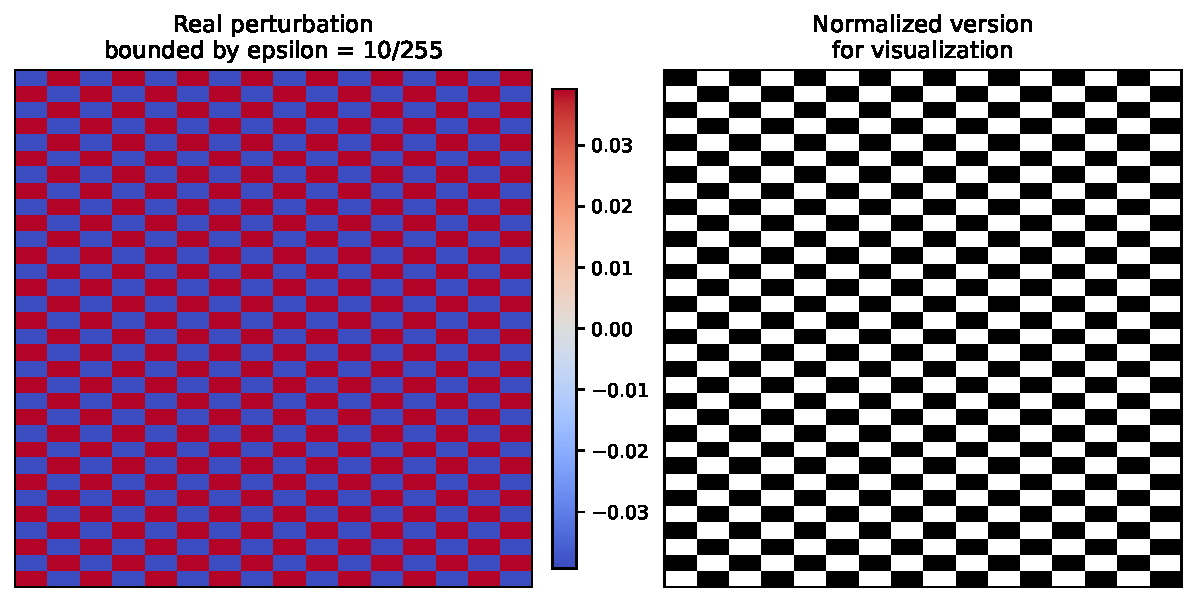
\includegraphics[width=0.55\textwidth]{figures/results/sfa_spatial_pattern_vgg_cifar10_en.pdf}
    \caption{Spatial pattern associated with the SFA perturbation at frequency $(16,24)$. The visualization is
    normalized to make the pattern's structure visible.}
    \label{fig:sfa_spatial_pattern_vgg_cifar10}
\end{figure}

\section{Measuring Frequency Sensitivity}
\label{sec:mesure_sensibilite_frequentielle}

Once the Fourier perturbations have been defined, their effect on the model must be measured.

\subsection{Definition of the Fool Ratio}
\label{subsec:def_fool_ratio}

Let $f$ be the model under study, and let $\mathcal{D}=\{x_1,\dots,x_M\}$ be a set of images. For a
given frequency $(u,v)$, let $\tilde{x}_k^{(u,v)}$ denote the image obtained by adding to $x_k$ the Fourier
perturbation associated with that frequency.

The \textit{fool ratio} measures the proportion of images for which the model's prediction changes
after perturbation:
\[
    \operatorname{FR}(u,v)
    =
    \frac{1}{M}
    \sum_{k=1}^{M}
    \mathbf{1}
    \left[
        f(x_k) \neq f\!\left(\tilde{x}_k^{(u,v)}\right)
    \right].
\]

This measure does not directly compare the prediction with the true label. It compares only the
model's prediction before and after perturbation. Thus, the attack counts as successful
on an image when the perturbation changes the model's decision.

The \textit{fool ratio} therefore indicates how effectively a frequency direction can change
predictions, regardless of the images' true class.

% \subsection{Stabilité entre heatmaps}

% Pour comparer les heatmaps obtenues avec différentes seeds d'entraînement, nous utilisons deux
% mesures de corrélation. Chaque heatmap est d'abord aplatie en un vecteur de taille $32\times32$,
% contenant les \textit{fool ratios} de toutes les fréquences.

% La corrélation de Pearson mesure si deux heatmaps ont une structure globale similaire en valeur. La
% corrélation de Spearman compare plutôt l'ordre relatif des fréquences, en remplaçant les valeurs par
% leurs rangs. Elle permet donc de vérifier si les fréquences les plus sensibles restent globalement les
% mêmes d'un entraînement à l'autre, même lorsque les valeurs exactes des \textit{fool ratios} changent
% légèrement.

\subsection{Generating Heatmaps}
\label{subsec:generation_heatmaps}

A frequency sensitivity heatmap is a matrix $H \in \mathbb{R}^{32\times32}$ in which each
entry corresponds to a frequency $(u,v)$. The value $H_{u,v}$ is the \textit{fool ratio} obtained when
the Fourier perturbation associated with that frequency is added to the test images.

The computation has three steps: first, we compute the model's predictions on clean images;
next, for each frequency, we apply the corresponding perturbation; finally, we measure
the proportion of predictions that change. This procedure is summarized in
Algorithm~\ref{algo:algorithme_heatmap}.

\begin{algorithm}[H]
\caption{Generating a frequency sensitivity heatmap}
\label{algo:algorithme_heatmap}
\begin{algorithmic}
\State \textbf{input}: model $f$, test images $\mathcal{D}$, amplitude $\epsilon$
\State \textbf{output}: heatmap $H \in \mathbb{R}^{32 \times 32}$
\State
\State $y \leftarrow f(\mathcal{D})$ \Comment{predictions on clean images}
\For{$u = 0$ \textbf{to} $31$}
    \For{$v = 0$ \textbf{to} $31$}
        \State $\delta_{u,v} \leftarrow$ construct the Fourier perturbation at frequency $(u,v)$
        \State $\tilde{\mathcal{D}}_{u,v} \leftarrow \operatorname{clip}_{[0,1]}(\mathcal{D} + \delta_{u,v})$
        \State $\tilde{y}_{u,v} \leftarrow f(\tilde{\mathcal{D}}_{u,v})$
        \State $H_{u,v} \leftarrow \operatorname{FoolRatio}(y,\tilde{y}_{u,v})$
    \EndFor
\EndFor
\end{algorithmic}
\end{algorithm}

\subsection{Selecting the Most Sensitive Frequency}
\label{subsec:choix_frequence_sensible}

Once the heatmap has been computed, we select the frequency that maximizes the \textit{fool ratio}:
\[
    (u^\star,v^\star)
    =
    \arg\max_{(u,v)}
    \operatorname{FR}(u,v).
\]

This frequency corresponds to the most effective Fourier perturbation among all those tested
in the protocol.

This selection is performed separately for CIFAR-10 and CIFAR-100. The resulting frequencies and
their interpretation are presented in Section~\ref{subsec:frequences_plus_sensibles}.

\section{Experimental Results}
\label{sec:resultats_experimentaux}

\subsection{Frequency Sensitivity Heatmaps}
\label{subsec:resultats_heatmaps}

The methodology described above allows us to construct frequency sensitivity maps
for the \texttt{VGGSmallBN} model. Figure~\ref{fig:heatmap_comparison_vgg_cifar10_cifar100}
compares the results obtained on our two datasets at the same perturbation amplitude,
set to $\epsilon = 10/255$.

\begin{figure}[H]
    \centering
    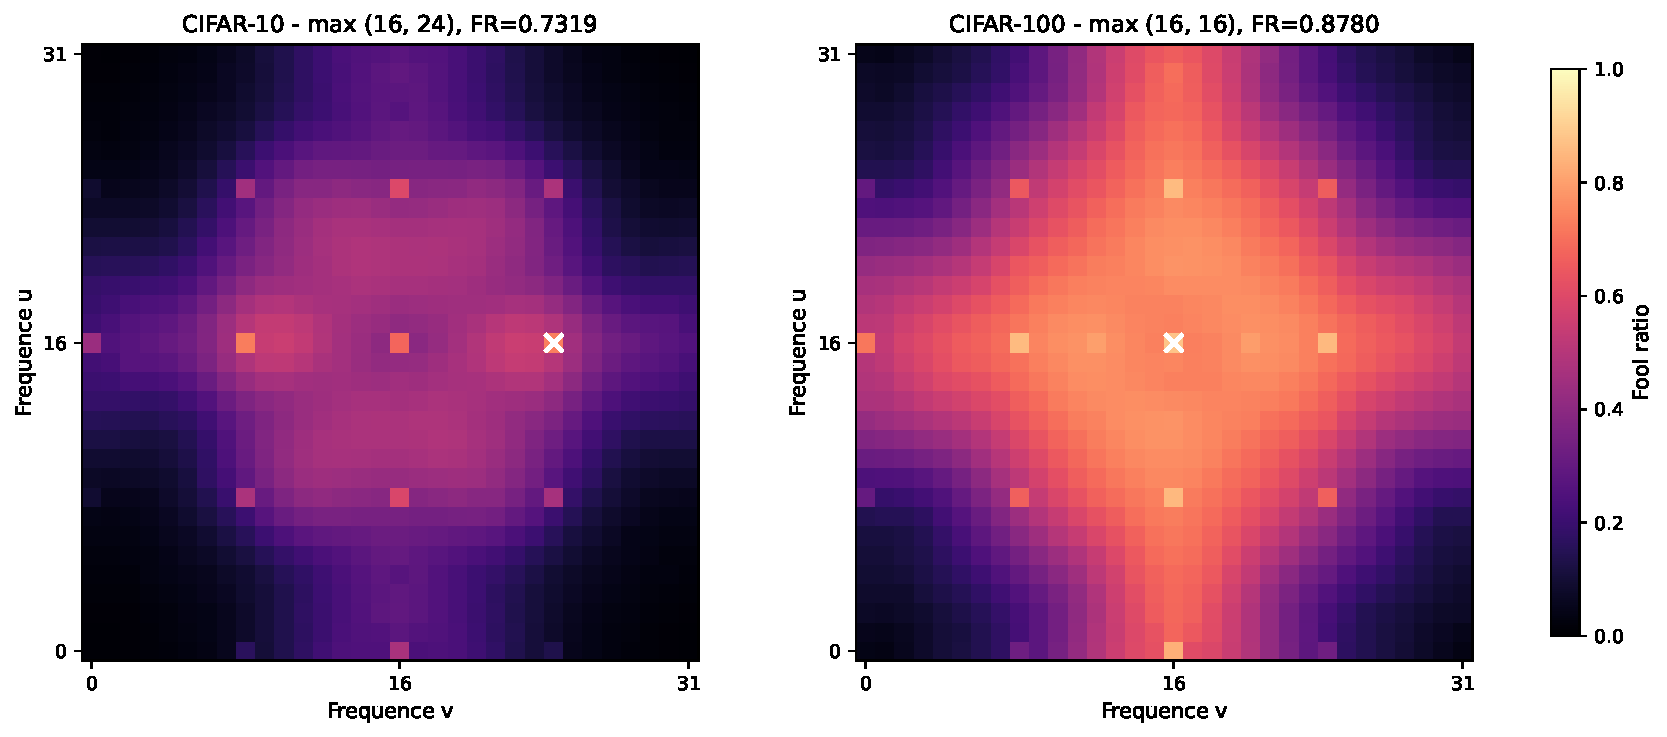
\includegraphics[width=0.7\textwidth]{figures/results/fourier_heatmap_comparison_vgg_cifar10_cifar100.pdf}
    \caption{Frequency sensitivity heatmaps for \texttt{VGGSmallBN} on CIFAR-10 and CIFAR-100.}
    \label{fig:heatmap_comparison_vgg_cifar10_cifar100}
\end{figure}
The main observation is that sensitivity is not uniform in the Fourier domain. Some
frequencies cause very few prediction changes, while others produce a
much higher \textit{fool ratio}.

Both heatmaps exhibit a structured organization, with regions of high sensitivity around
certain frequency lines and intersections, particularly near coordinates associated with $16$. This
structure suggests that the model's vulnerability is not a random effect, but depends on certain
preferred frequency directions.

A descriptive comparison with the mean spectrum of clean images appears in
Appendix~\ref{annexe:spectres_moyens_cifar}. This analysis aims to offer another way of interpreting
the results through the frequency statistics of the raw data.

To complement the heatmaps, Figure~\ref{fig:fool_ratio_histogram_comparison_vgg_cifar10_cifar100}
shows the distribution of \textit{fool ratios} over the $32 \times 32 = 1024$ frequencies tested.

On CIFAR-10, most frequencies have a weak or moderate effect, and only a few directions
achieve high \textit{fool ratios}. The model's sensitivity is therefore real, but relatively
localized in the frequency domain.

\begin{figure}[H]
    \centering
    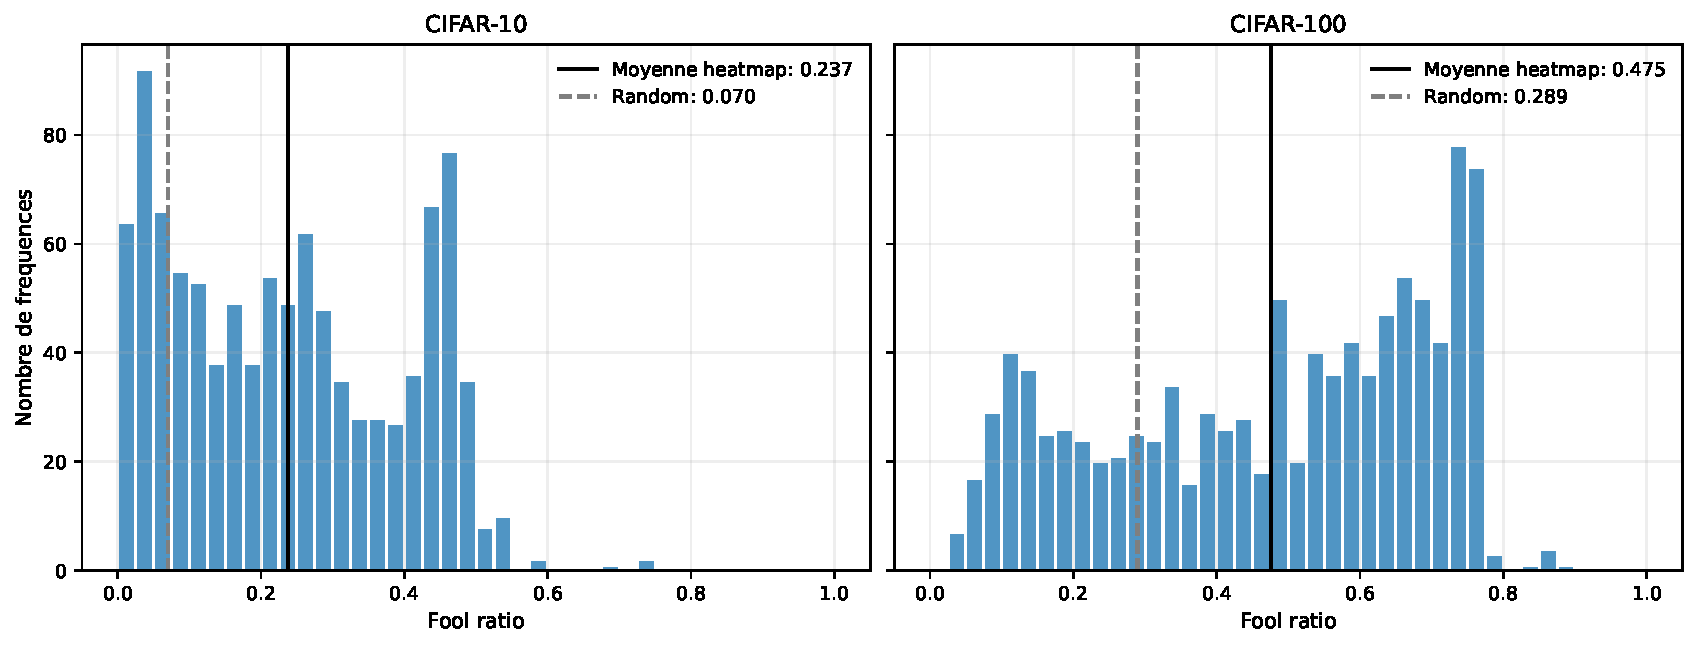
\includegraphics[width=0.9\textwidth]{figures/results/fourier_fool_ratio_histogram_comparison_vgg_cifar10_cifar100.pdf}
    \caption{Distribution of the \textit{fool ratios} obtained over all Fourier frequencies tested.}
    \label{fig:fool_ratio_histogram_comparison_vgg_cifar10_cifar100}
\end{figure}

On CIFAR-100, the distribution shifts to the right: the mean increases from $0.2375$ to $0.4755$.
The model is therefore more fragile overall, consistent with the greater difficulty of the
task discussed in Appendix~\ref{annexe:marges-logits}. However, this fragility remains structured: not all frequencies produce the same
effect, and some directions remain markedly more disruptive than others.

The histogram thus complements the visual interpretation of the heatmaps. It shows that sensitivity is
not only spatially nonuniform but also quantitatively highly dispersed. A small fraction
of the frequencies accounts for most of the disruptive effect.

\subsection{Most Sensitive Frequencies}
\label{subsec:frequences_plus_sensibles}

Analysis of the heatmaps identifies the most disruptive frequencies for each
dataset. Table~\ref{tab:frequences_plus_sensibles} presents the three frequencies with the
highest \textit{fool ratios}.

\begin{table}[H]
    \centering
    \begin{tabular}{c|cc|cc}
        & \multicolumn{2}{c|}{CIFAR-10} & \multicolumn{2}{c}{CIFAR-100} \\
        Rank & Frequency $(u,v)$ & \textit{Fool ratio} & Frequency $(u,v)$ & \textit{Fool ratio} \\
        \hline
        1 & $(16,24)$ & $0.7319$ & $(16,16)$ & $0.8780$ \\
        2 & $(16,8)$  & $0.7295$ & $(16,8)$  & $0.8585$ \\
        3 & $(16,16)$ & $0.6765$ & $(24,16)$ & $0.8565$ \\
    \end{tabular}
    \caption{Most sensitive frequencies for \texttt{VGGSmallBN} on CIFAR-10 and CIFAR-100.}
    \label{tab:frequences_plus_sensibles}
\end{table}

The dominant frequencies cluster around the same family of directions. On CIFAR-10, the top two frequencies,
$(16,24)$ and $(16,8)$, are conjugates modulo $32$ and, as expected, yield almost identical \textit{fool ratios}.


On CIFAR-100, the most sensitive frequency becomes $(16,16)$, which is its own conjugate modulo
$32$.

\subsection{Stability of Sensitive Regions Across Training Runs}
\label{subsec:stabilite_multi_seeds}

The preceding heatmaps show that some frequencies are much more sensitive than
others. However, an important question remains: is this structure specific to a
particular training run, or does it remain observable when the initialization seed
changes?

\begin{figure}[H]
    \centering
    \vspace{-10pt} 

    \begin{minipage}{0.35\textwidth}
        \centering
        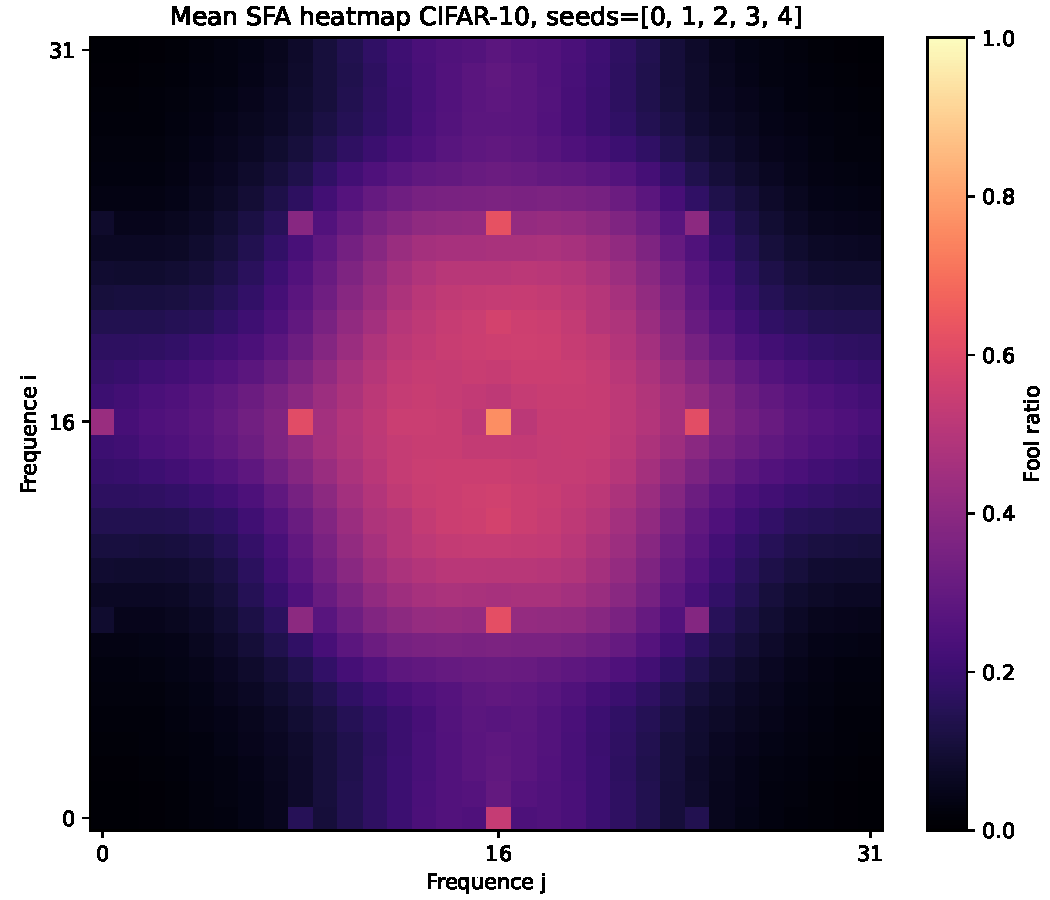
\includegraphics[width=\textwidth]{figures/results/stability_cifar10_heatmap_mean.pdf}
        \vspace{-5pt} 
        {\small (a) CIFAR-10 -- mean \textit{fool ratio}}
    \end{minipage}
    \hspace{0.05\textwidth} 
    \begin{minipage}{0.35\textwidth}
        \centering
        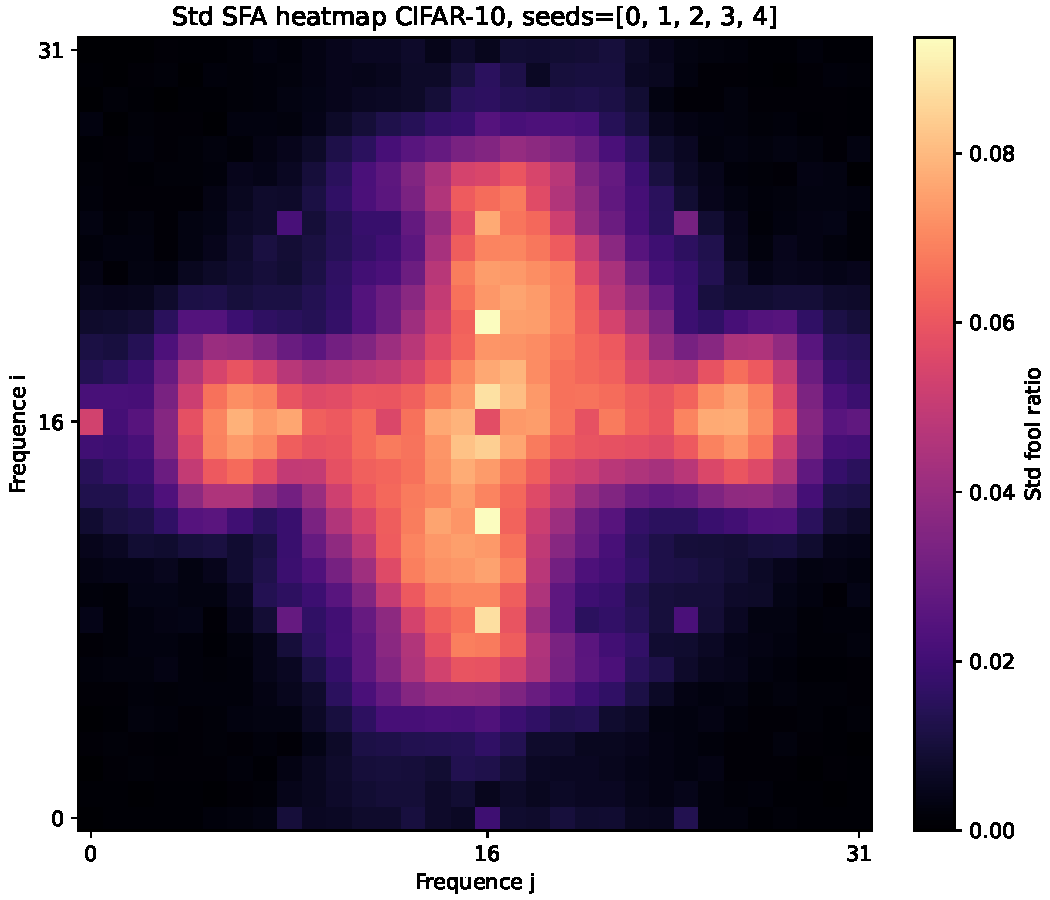
\includegraphics[width=\textwidth]{figures/results/stability_cifar10_heatmap_std.pdf}
        \vspace{-5pt}
        {\small (b) CIFAR-10 -- standard deviation}
    \end{minipage}

    \vspace{2pt} 

    \begin{minipage}{0.35\textwidth}
        \centering
        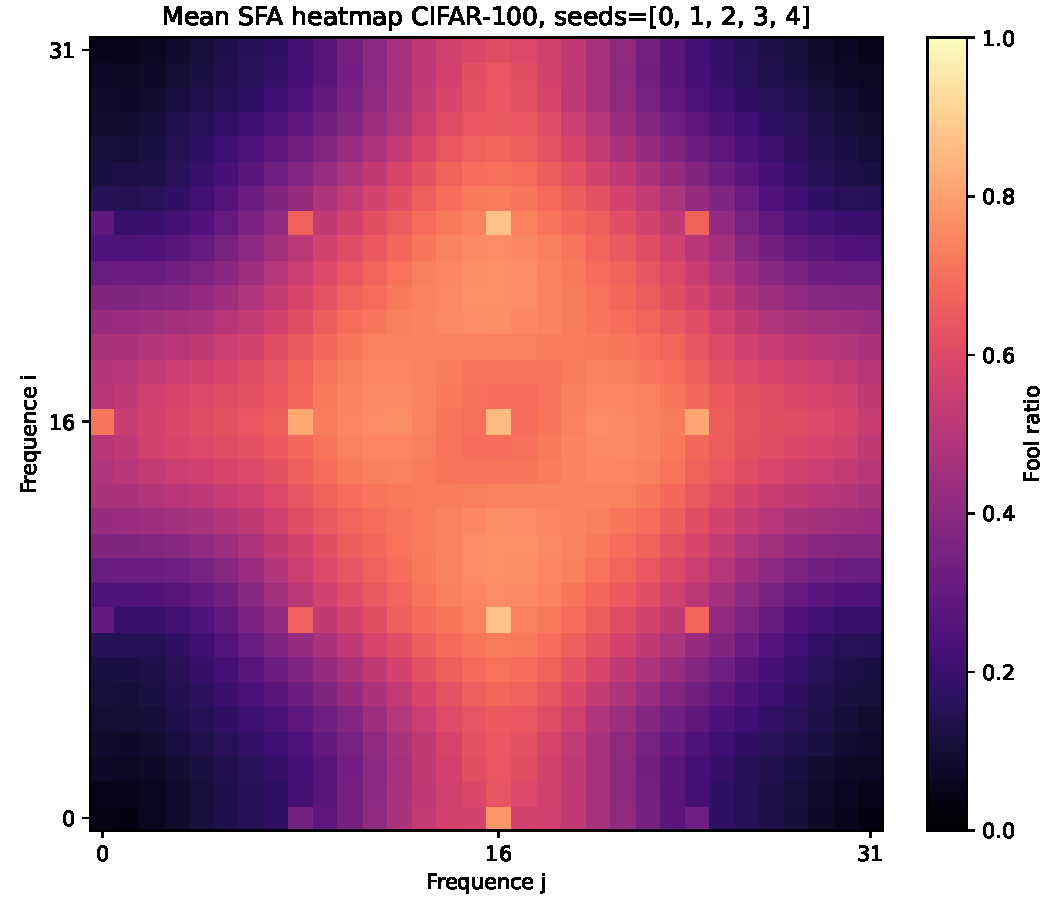
\includegraphics[width=\textwidth]{figures/results/stability_cifar100_heatmap_mean.pdf}
        \vspace{-5pt}
        {\small (c) CIFAR-100 -- mean \textit{fool ratio}}
    \end{minipage}
    \hspace{0.05\textwidth}
    \begin{minipage}{0.35\textwidth}
        \centering
        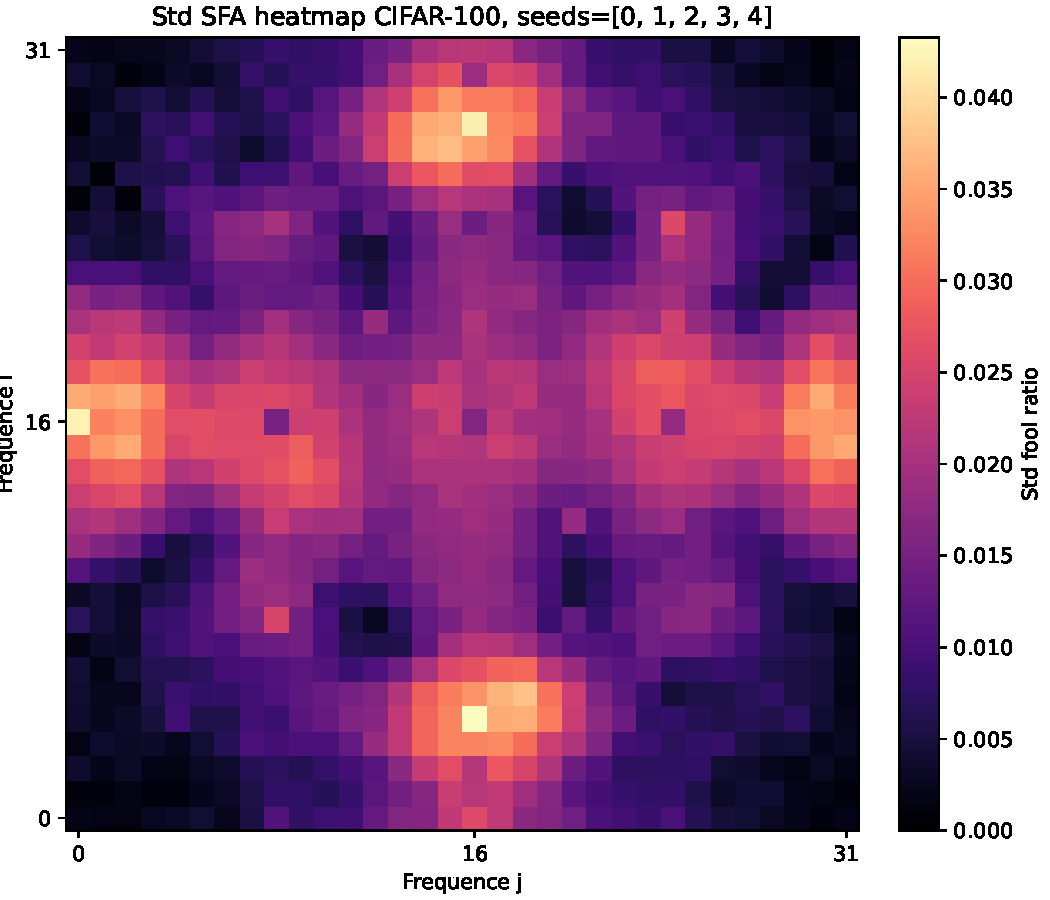
\includegraphics[width=\textwidth]{figures/results/stability_cifar100_heatmap_std.pdf}
        \vspace{-5pt}
        {\small (d) CIFAR-100 -- standard deviation}
    \end{minipage}

    \caption{Stability of the frequency sensitivity of \texttt{VGGSmallBN} on CIFAR-10 and CIFAR-100.}
    \label{fig:stability_cifar10_cifar100_mean_std}
\end{figure}

To answer this question, we repeated the experiment on CIFAR-10 and CIFAR-100 with five
independent training runs of \texttt{VGGSmallBN}. The training protocol remains identical
for each run. Only the seed changes.

For each dataset, Figure~\ref{fig:stability_cifar10_cifar100_mean_std} presents
the mean heatmap obtained across the five seeds and the standard deviation associated
with each frequency.

The results show that the overall heatmap structure remains highly stable across training runs.
On CIFAR-10, regions of high sensitivity remain localized around the same frequency regions,
particularly around the middle frequencies associated with the central axes. On CIFAR-100, this structure
is even more pronounced: a broad region of high sensitivity appears around the central frequencies.

% Cette stabilité est confirmée quantitativement par les corrélations entre heatmaps. Sur CIFAR-10, la
% corrélation de Pearson moyenne entre heatmaps est d'environ $0.976$, et la corrélation de Spearman
% moyenne d'environ $0.985$. Sur CIFAR-100, ces valeurs montent respectivement à environ $0.994$
% et $0.992$. Les heatmaps sont donc très proches d'un entraînement à l'autre, aussi bien en valeur
% qu'en classement relatif des fréquences.

Table~\ref{tab:stability_multiseed_metrics} summarizes the main metrics averaged across the five
seeds. Clean accuracy remains close to that of the main model, whereas accuracy after the attack
drops sharply. This shows that the high \textit{fool ratio} does correspond to an actual degradation
of model performance, rather than merely to prediction changes that have no effect on
correct classification.

\begin{table}[H]
    \centering
    \begin{tabular}{l|c|c}
        \hline
        Metric & CIFAR-10 & CIFAR-100 \\
        \hline
        Mean clean accuracy & $93.08\,\%$ & $72.50\,\%$ \\
        Mean best \textit{fool ratio} & $76.35\,\%$ & $87.64\,\%$ \\
        Mean accuracy after attack & $23.39\,\%$ & $11.83\,\%$ \\
        Success rate on initially correct images & $76.38\,\%$ & $85.18\,\%$ \\
        % Corrélation de Pearson moyenne entre heatmaps & $0.976$ & $0.994$ \\
        % Corrélation de Spearman moyenne entre heatmaps & $0.985$ & $0.992$ \\
        \hline
    \end{tabular}
    \caption{Summary of the stability experiment across multiple seeds on CIFAR-10 and CIFAR-100.}
    \label{tab:stability_multiseed_metrics}
\end{table}

\subsection{Internal Amplification of Sensitive Frequencies}
\label{subsec:amplification_interne_sfa}

The preceding heatmaps show that some Fourier frequencies produce markedly higher \textit{fool ratios}
than others. To better understand this phenomenon, we analyzed how
these perturbations propagate inside the network.

For a perturbation \(\delta\), let \(G_l(\delta)\) denote the normalized amplification measured at
layer \(l\). This quantity compares the mean norm of the activation change caused by the
perturbation with the norm of the input perturbation. It therefore allows us to compare the relative effect of
different frequencies within the network's internal blocks and at the logit level.

To make this analysis more robust, we repeated it on the five checkpoints used in
the stability experiment across multiple seeds. Frequencies are grouped using the mean heatmap:
the \(50\) most sensitive frequencies, \(50\) frequencies of intermediate sensitivity, and the \(50\)
least sensitive frequencies. The primary frequency is the best frequency on average
across the five seeds.

\begin{figure}[H]
    \centering
    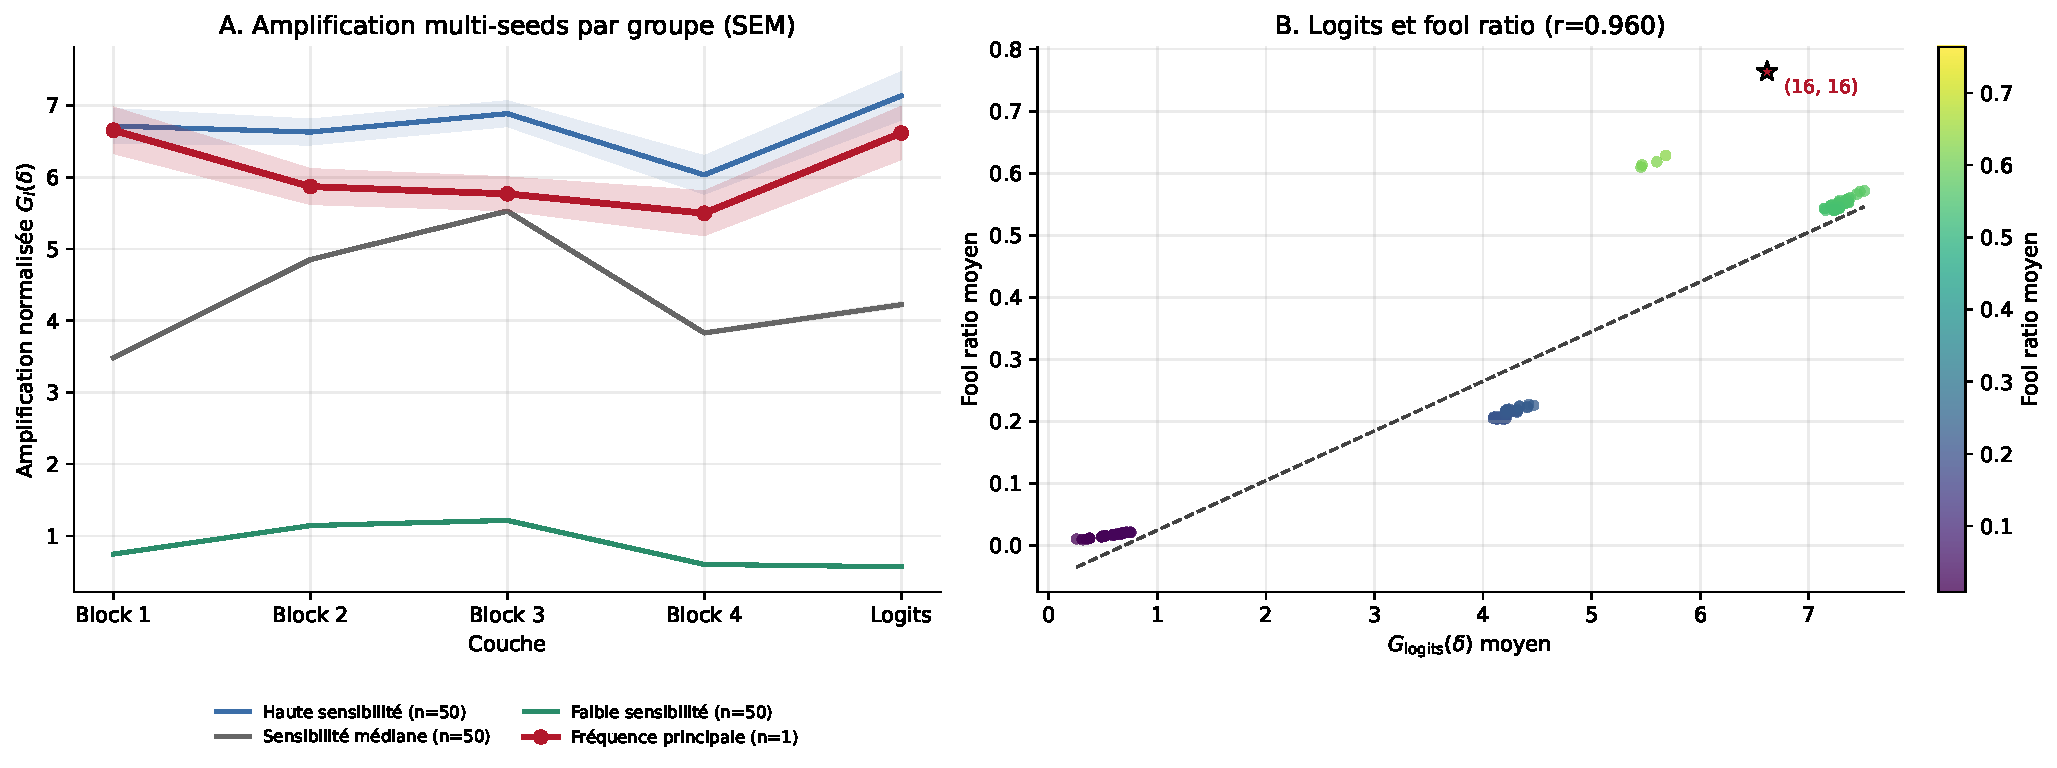
\includegraphics[width=\textwidth]{figures/results/layerwise_frequency_sensitivity_analysis_vgg_cifar10_multiseed.pdf}
    \caption{Analysis of the internal amplification of Fourier perturbations across multiple seeds in
    \texttt{VGGSmallBN} on CIFAR-10. Left: frequencies are grouped by their
    mean \textit{fool ratio}. Bands indicate the standard error across the five seeds. Right:
    mean amplification at the logit level is compared with the mean \textit{fool ratio}.}
    \label{fig:layerwise_frequency_sensitivity_multiseed}
\end{figure}

Figure~\ref{fig:layerwise_frequency_sensitivity_multiseed} shows that, as expected, the most
sensitive frequencies also produce the greatest internal amplification.

The right panel shows a strong correlation between mean amplification at the logit level
and the mean \textit{fool ratio}. This suggests that the model's final sensitivity is related not only
to the chosen pair $(u, v)$, but also to how this perturbation is propagated and
amplified by the network.

This observation connects with the theoretical framework and the local interpretation introduced in the
previous chapter: although the real network is not globally linear, certain
frequency directions seem to be amplified more by its local behavior, which may explain
their greater effect on predictions.

A more detailed visualization of the internal heatmaps by layer is provided in Appendix~\ref{annexe:heatmaps_internes_couches}.

\subsection{Comparison with Random Noise}
\label{subsec:comparaison_bruit_aleatoire}

To verify that the high values obtained by SFA are not solely due to the perturbation's
amplitude, we compare the best Fourier direction with a random-noise
baseline. In this baseline, each pixel is perturbed independently by uniform noise
bounded within the same amplitude interval. The constraint is therefore the same as for SFA:
\[
    \|\delta\|_{\infty} \leq \epsilon,
    \qquad
    \epsilon = 10/255.
\]
The difference lies in the perturbation's structure: SFA uses a coherent frequency pattern,
whereas the random baseline does not favor any particular direction.

\textbf{TO DO: }
We should ensure that $\|\delta_{SFA}\|_{2} = \|\delta_{random}\|_{2}$

For each dataset, Figure~\ref{fig:sfa_vs_random_comparison_vgg_cifar10_cifar100} compares
the \textit{fool ratio} of the best SFA frequency with the mean \textit{fool ratio} obtained using random
noise.

\begin{figure}[H]
    \centering
    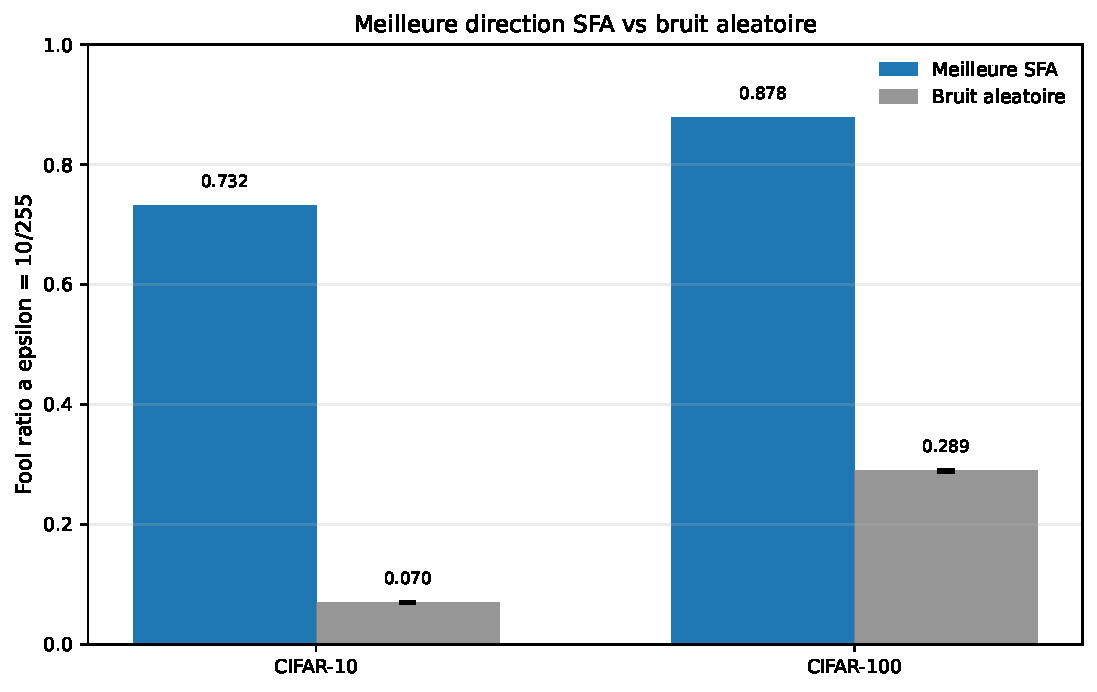
\includegraphics[width=0.85\textwidth]{figures/results/sfa_vs_random_comparison_vgg_cifar10_cifar100.pdf}
    \caption{Comparison between the best SFA direction and uniform random noise of the same amplitude
    $\epsilon = 10/255$. For random noise, the error bar represents the standard deviation over 100 trials.}
    \label{fig:sfa_vs_random_comparison_vgg_cifar10_cifar100}
\end{figure}

On CIFAR-10, the difference is striking: the best Fourier direction achieves a
\textit{fool ratio} of $0.7319$, whereas the mean for random noise is only $0.0704$.
The Fourier perturbation is therefore approximately ten times as effective as random noise of the same
amplitude. This result indicates that the observed vulnerability cannot be explained solely by
the size of the perturbation.

On CIFAR-100, random noise is already more disruptive, with a mean \textit{fool ratio} of
$0.2892$, confirming that the model trained on CIFAR-100 is more fragile overall. However,
the best SFA direction reaches $0.8780$, approximately three times the mean level for random noise.

\subsection{Effect of Perturbation Amplitude}
\label{subsec:effet_amplitude_epsilon}

So far, the main results have been obtained with $\epsilon = 10/255$. This value allows us to
compare our results with the original protocol, but it can produce visible patterns in
very low-resolution images. However, an adversarial attack aims to remain
barely perceptible to humans. We therefore test whether the most sensitive frequencies retain an effect at
lower values of $\epsilon$.

To do so, we fix the most sensitive frequency for each dataset and then vary
$\epsilon$ over the following set:
\[
    \epsilon \in
    \left\{
        \frac{1}{255},
        \frac{2}{255},
        \frac{3}{255},
        \frac{5}{255},
        \frac{10}{255}
    \right\}.
\]

\begin{figure}[H]
    \centering
    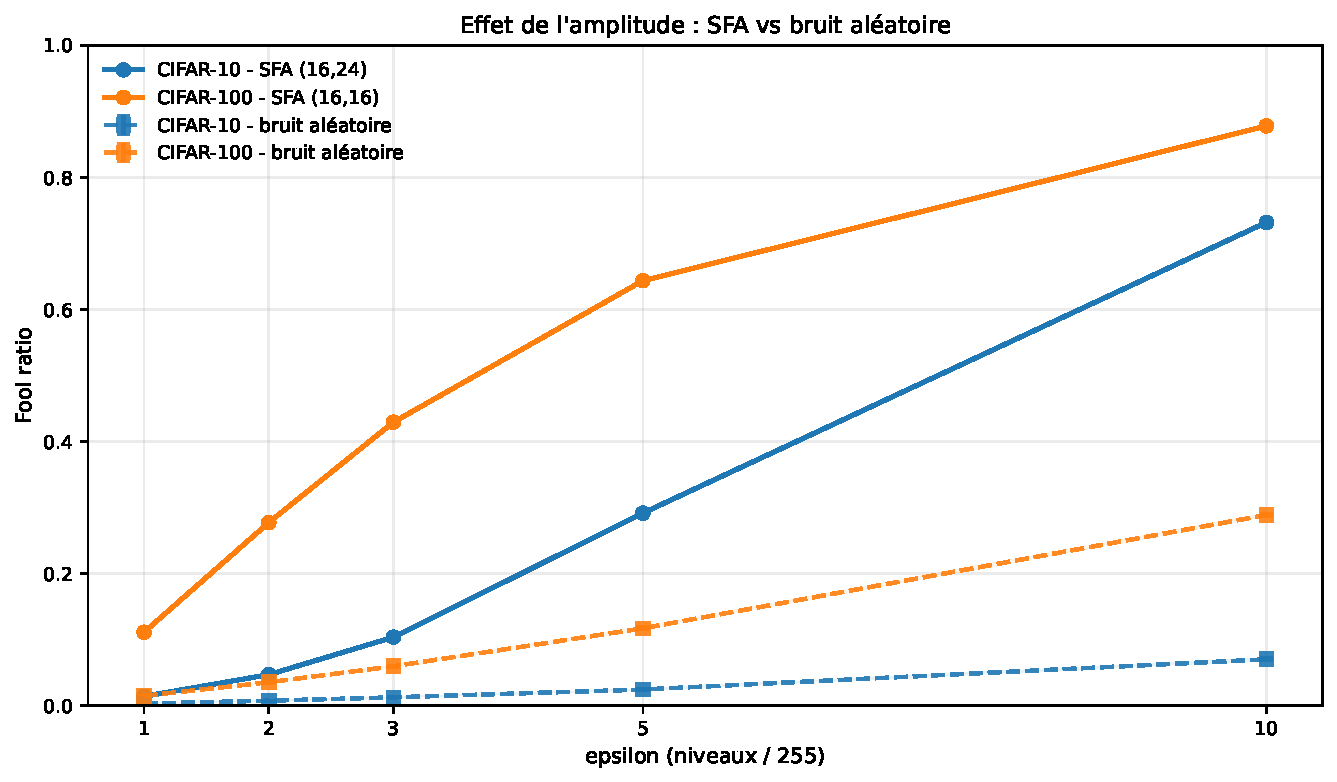
\includegraphics[width=0.55\textwidth]{figures/results/sfa_epsilon_sweep_with_random_comparison_vgg_cifar10_cifar100.pdf}
    \caption{\textit{Fool ratio} as a function of amplitude $\epsilon$ for the best SFA frequency
    on each dataset.}
    \label{fig:sfa_epsilon_sweep_comparison_vgg_cifar10_cifar100}
\end{figure}

Figure~\ref{fig:sfa_epsilon_sweep_comparison_vgg_cifar10_cifar100} shows a steady
increase in the \textit{fool ratio} as $\epsilon$ increases. This behavior is expected: the larger the
perturbation, the more it changes the input image and the more likely it is to alter the
model's prediction. However, it also confirms that, in this setting, perturbation amplitude
is an important factor in attack effectiveness, requiring a less subtle perturbation
to obtain a more substantial effect.

\begin{figure}[H]
    \centering
    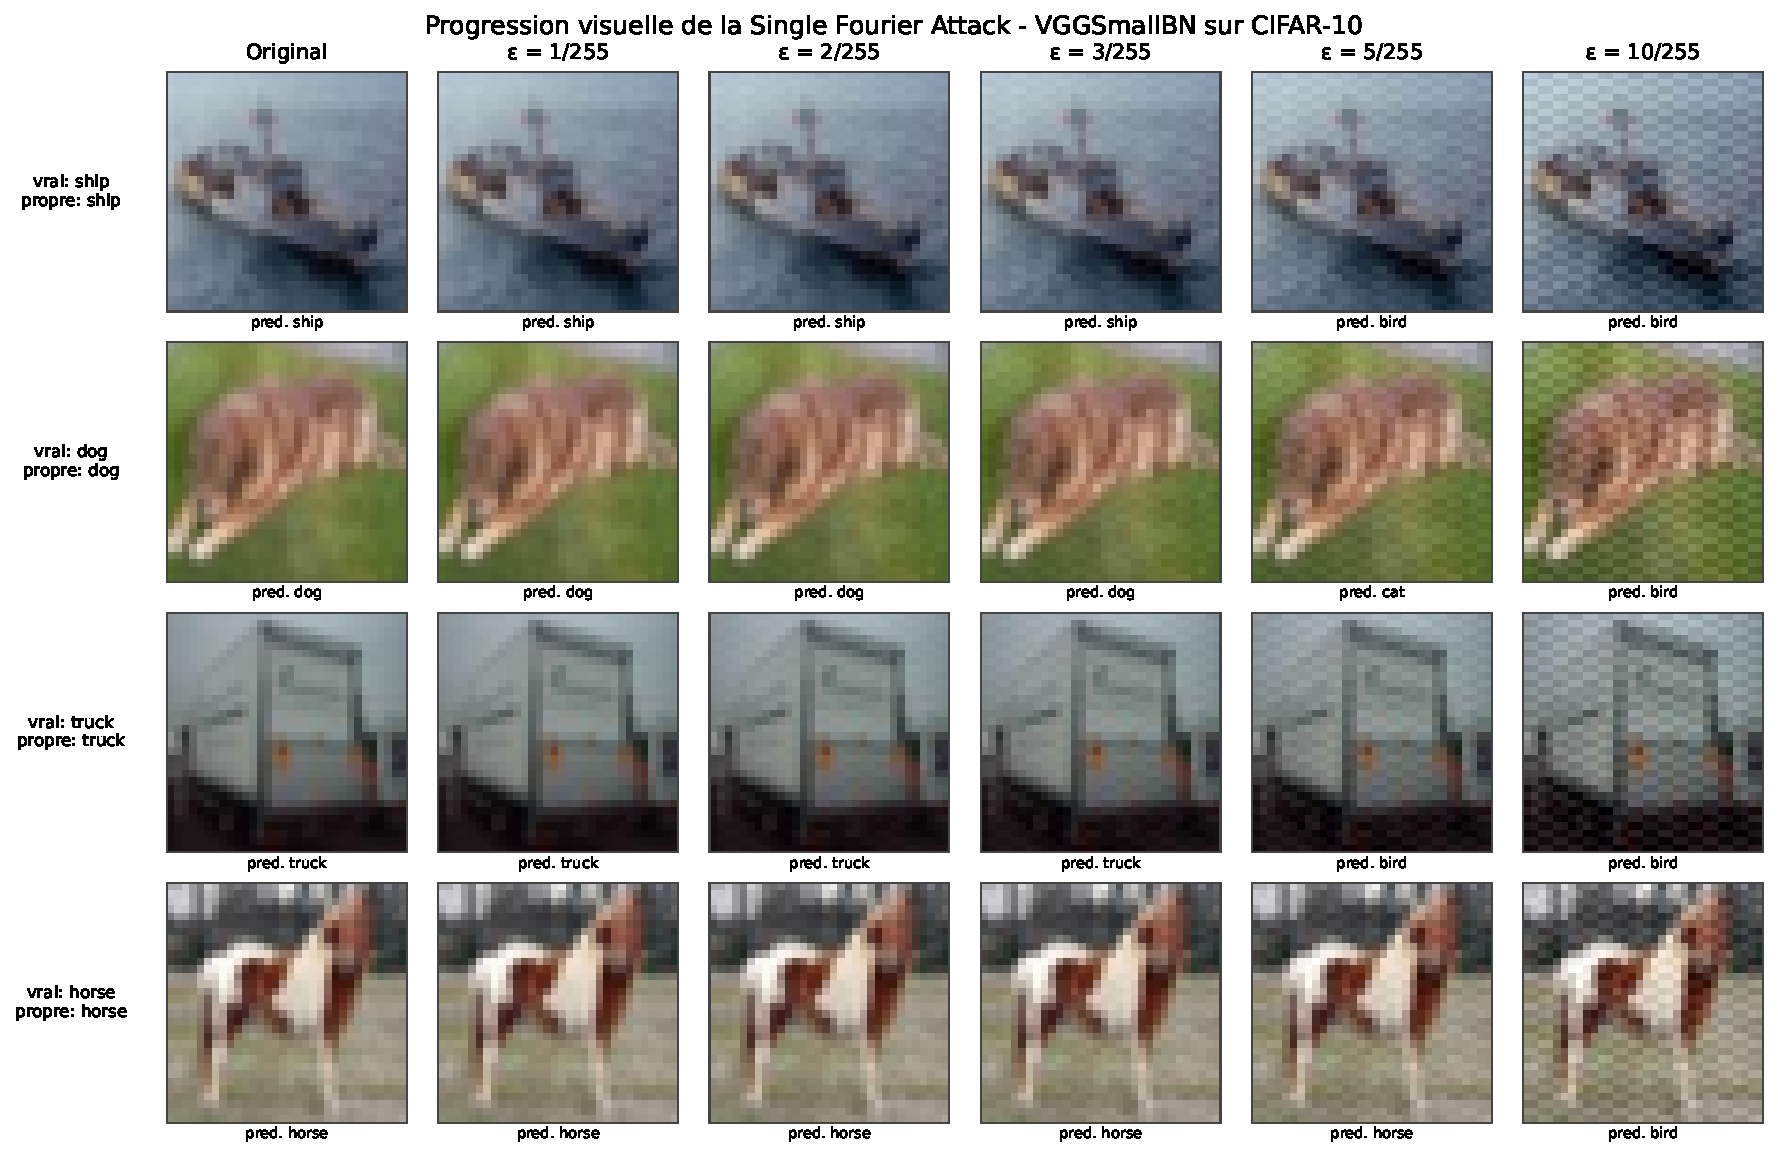
\includegraphics[width=1\textwidth]{figures/results/sfa_visual_progression_vgg_cifar10.pdf}
    \caption{Visual progression of a \textit{Single Fourier Attack} on CIFAR-10 images.}
    \label{fig:sfa_visual_progression_vgg_cifar10}
\end{figure}

As Figure~\ref{fig:sfa_visual_progression_vgg_cifar10} illustrates, increasing the amplitude makes the
Fourier pattern increasingly intrusive. In particular, from $\epsilon = 3/255$ onward, the
structured grid-like perturbation begins to become clearly visible to the naked eye.

These observations should nevertheless be qualified. The experiments use
very low-resolution images ($32\times32$ pixels) and a deliberately limited architecture
(\texttt{VGGSmallBN}). The conclusions should therefore not be generalized directly to
high-resolution images or much deeper architectures. They do, however, show that,
in our experimental setting, the effect of Fourier perturbations depends strongly on amplitude.

\subsection{Connection with the Theoretical Framework}
\label{subsec:discussion_lien_cadre_theorique}

The experimental results in this chapter allow us to revisit the theoretical framework
developed in the previous chapter. In the idealized linear model, Fourier functions emerge
as preferred directions of convolution operators. In a real CNN, this property
no longer applies directly to the entire network, but it may remain locally relevant through
the model's Jacobian.

The experimental heatmaps support this interpretation. If all frequency directions
were equivalent for the model, the sensitivity maps would be much more uniform. Yet this
is not what we observe: some frequencies produce markedly higher \textit{fool ratios}
than others, even though all perturbations satisfy the same $\ell_\infty$ constraint.

Stability across multiple seeds reinforces this interpretation. The sensitive regions do not seem to depend
solely on a particular network initialization: they remain visible when training is
repeated with different seeds. The comparison with random noise also shows that the effect
arises not only from the perturbation's amplitude, but also from its frequency structure.

These results show that the intuition derived from the theoretical framework remains
experimentally observable for \texttt{VGGSmallBN}: some Fourier directions are more disruptive than others,
consistent with local amplification of these directions within the network.

\paragraph{Influence of channel mixing.}

Previously, we considered the possibility that a sensitive direction may also involve mixing
the color channels, in the form $a \otimes \varphi_{u,v}$. The main protocol uses a simplified version of
this idea: the same Fourier pattern is applied to all three channels, corresponding to a
color direction of the form $(1,1,1)$.

A supplementary analysis of this simplification is provided in Appendix~\ref{annexe:color_sfa}.
It aims to show that the choice of channel mixing has a negligible effect compared with selecting the direction that maximizes attack amplification.

\section{Chapter Summary}
\label{sec:synthese_chapitre4}

The experiments confirm that the sensitivity of \texttt{VGGSmallBN} to Fourier
perturbations is highly nonuniform. On both CIFAR-10 and CIFAR-100, some frequencies
cause far more prediction changes than others, even though all perturbations
satisfy the same $\ell_\infty$ constraint.

This structure remains stable across several independent training runs and substantially exceeds the effect
of random noise of the same amplitude. However, the $\epsilon$ sweep shows that
attack effectiveness depends strongly on amplitude, particularly for low-resolution
images such as those in CIFAR.

Finally, the internal analysis suggests that the most sensitive frequencies are also those amplified
most strongly in the network's representations. These observations do not prove that the real model
behaves as a global linear operator, but they show that the frequency structure
identified in the theoretical setting remains partly visible in the model's local behavior.

\chapter{Conclusion}

This work aimed to explore the intrinsic connection between the convolutional structure of neural
networks (CNNs) and the emergence of preferred directions of vulnerability in the
Fourier domain. More specifically, our approach sought to determine the extent to which the
mathematical properties inherent in convolutional layers, beyond biases associated with the data or
the training process, can explain the existence of universal adversarial perturbations.

To this end, after establishing the general framework of CNNs and adversarial attacks, we
reconstructed and analyzed the theoretical reasoning proposed by Tsuzuku and
Sato~\cite{tsuzuku2019structural}, initially using a simplified linear model.

To extend these theoretical results to actual CNN architectures, where
ReLU activations and \textit{max-pooling} operations prevent any
global diagonalization, we introduced local linearization through
analysis of the model's Jacobian. This theoretical extension proved crucial
in justifying the application of results based on linearity to
fundamentally nonlinear architectures.

Together, these observations clarify the mechanism by which a
perturbation based on a single Fourier frequency can affect a convolutional
network so severely. The successive amplification of this perturbation through
the different layers provides a compelling structural explanation for the existence of
universal perturbations.

Our experimental approach supports this intuition. The \textit{heatmaps}
obtained for \texttt{VGGSmallBN} on the CIFAR-10 and
CIFAR-100 datasets reveal highly heterogeneous frequency sensitivity.
Certain frequencies produce significantly higher \textit{fool ratios},
showing that perturbations of equal amplitude do not have an
equivalent impact: their direction in input space is a determining factor.
Comparison with random noise of the same amplitude
fully corroborates this asymmetry.

The results also highlight the expected influence of classification task
complexity on model robustness. Overall, the network proves more
vulnerable on CIFAR-100 than on CIFAR-10. This vulnerability, examined in greater detail
in Appendix~\ref{annexe:marges-logits}, is consistent with the increased difficulty of the problem:
with more classes, decision boundaries become more numerous and more closely
spaced because of the visual similarity between categories, allowing a perturbation
to change the prediction more easily. Nevertheless, despite this increased vulnerability,
sensitivity retains a structured topology in which certain Fourier directions remain dominant.

The scope of these results should nevertheless be interpreted cautiously. Our experimental reproduction
is limited to a VGG-type architecture and low-resolution images. Moreover, the
most sensitive frequencies were selected from \textit{heatmaps} computed on
the test set. We therefore cannot claim that all convolutional networks exhibit
exactly the same vulnerability structure. Within the setting studied here, however, Fourier
directions appear to be a useful tool for better understanding certain sensitivities of CNNs.

This analysis can also be related to model explainability. When a
particular frequency substantially changes the network's predictions, this indicates that this component
of the image plays an important role in its decision. In other words, sensitive frequencies
are useful not only for constructing adversarial perturbations: they also provide clues
about the type of information the network uses to classify images.

A possible continuation of this work would therefore be to use these sensitive frequencies both to strengthen
models and to interpret them more effectively. For example, they could guide new
forms of data augmentation, limit certain internal amplifications, or support comparisons of
more robust architectures, particularly those incorporating anti-aliasing mechanisms.

This direction would connect three important aspects: adversarial robustness,
resistance to variations in the data, and interpretation of the network's decisions.
The goal would therefore be not only to show that certain Fourier frequencies are dangerous
for the model, but also to understand how identifying them can help build networks
that are more stable, more robust, and more interpretable.



% {
\thispagestyle{empty}
\setstretch{1.2}
\fontsize{12pt}{14.4pt}\selectfont

\cleardoublepage
\addcontentsline{toc}{chapter}{Déclaration d'utilisation de l'IA}

\begin{tikzpicture}[remember picture, overlay]
    \node[opacity=0.08] at (current page.center) {
        
\includegraphics[width=0.7\textwidth]{formalisme/logo_unige.png} 
    };
\end{tikzpicture}

\vspace*{\fill} 

\begin{center}
    {\huge \bfseries Déclaration d'utilisation de l'IA} \\[3em]

    \begin{minipage}{0.85\textwidth}
        \centering
        Dans un souci de transparence et d'intégrité académique, l'auteur déclare avoir eu recours à des outils d'intelligence artificielle générative (\textbf{Gemini 3} et \textbf{ChatGPT 5.5}) comme assistance ponctuelle durant la rédaction de ce rapport.
        
        \vspace{2em}
        
        \raggedright
        L'utilisation de ces outils a porté sur les tâches suivantes :
        \begin{itemize}[label=\textbullet]
            \item \textbf{Relecture et formulation :} correction orthographique, amélioration grammaticale, reformulation de phrases et fluidification de certains passages.
            \item \textbf{Support LaTeX et TikZ :} assistance à la mise en forme du document, à la production de figures techniques et à la résolution de problèmes de compilation.
        \end{itemize}
        
        \vspace{2em}
        \centering

        L'auteur reste le seul responsable des décisions scientifiques, de l'assimilation des articles, du protocole expérimental, de l'interprétation des résultats et, bien sûr, du rendu final de ce rapport.        
    \end{minipage}
\end{center}

\vspace*{\fill} 
\newpage
}

\appendix
\chapter{Matrix Representation of a Linear Map}
\label{app:representation-lineaire-matrice}

Let $V$ and $W$ be two finite-dimensional vector spaces over a field
$\mathbb{K}$, where $\mathbb{K}$ denotes either $\mathbb{R}$ or $\mathbb{C}$.
Let
\[
\mathcal{B} = (e_1,\dots,e_N)
\]
be a basis of $V$, and
\[
\mathcal{B}' = (e'_1,\dots,e'_M)
\]
a basis of $W$.

Now consider a linear map
\[
f : V \rightarrow W.
\]
Every vector $v \in V$ has a unique decomposition in the basis $\mathcal{B}$:
\[
v = \sum_{i=1}^{N} \alpha_i e_i,
\]
where the coefficients $\alpha_i$ are the coordinates of $v$ in the basis $\mathcal{B}$.

By linearity of $f$,
\[
f(v)
=
f\left(\sum_{i=1}^{N} \alpha_i e_i\right)
=
\sum_{i=1}^{N} \alpha_i f(e_i).
\]

Since $f(e_i) \in W$, each vector $f(e_i)$ can itself be decomposed in the basis
$\mathcal{B}'$. There therefore exist scalars $a_{j i} \in \mathbb{K}$ such that
\[
f(e_i)
=
\sum_{j=1}^{M} a_{j i} e'_j.
\]

Substituting this expression into the preceding formula gives
\[
f(v)
=
\sum_{i=1}^{N} \alpha_i
\left(
\sum_{j=1}^{M} a_{j i} e'_j
\right).
\]

Rearranging the sums according to the vectors of the basis $\mathcal{B}'$ yields
\[
f(v)
=
\sum_{j=1}^{M}
\left(
\sum_{i=1}^{N} a_{j i}\alpha_i
\right)
e'_j.
\]

If we write
\[
[f(v)]_{\mathcal{B}'}
=
\begin{pmatrix}
\beta_1 \\
\vdots \\
\beta_M
\end{pmatrix},
\qquad
[v]_{\mathcal{B}}
=
\begin{pmatrix}
\alpha_1 \\
\vdots \\
\alpha_N
\end{pmatrix},
\]
then the coordinates of $f(v)$ satisfy
\[
\beta_j
=
\sum_{i=1}^{N} a_{j i}\alpha_i.
\]

We can therefore write this in matrix form as
\[
[f(v)]_{\mathcal{B}'}
=
A [v]_{\mathcal{B}},
\]
where
\[
A =
(a_{j i})_{\substack{1 \leq j \leq M \\ 1 \leq i \leq N}}
\in \mathbb{K}^{M \times N}.
\]

In other words, the matrix $A$ representing the linear map $f$ is constructed column
by column: its $i$-th column is the coordinate vector of $f(e_i)$ in the basis
$\mathcal{B}'$:
\[
A
=
\begin{pmatrix}
| & | &        & | \\
[f(e_1)]_{\mathcal{B}'} & [f(e_2)]_{\mathcal{B}'} & \cdots & [f(e_N)]_{\mathcal{B}'} \\
| & | &        & |
\end{pmatrix}.
\]

Thus, every linear map between finite-dimensional vector spaces can be
represented by a matrix once a basis has been chosen for the domain
and a basis for the codomain.

This matrix depends on the choice of bases. The same linear
map can therefore have different matrix representations depending on the bases used.

\chapter{Eigenvectors, Eigenvalues, and Diagonalization}
\label{app:vecteurs-propres-diagonalisation}

Let $V$ be a vector space of finite dimension $N$ over a field $\mathbb{K}$, and let
\[
f : V \rightarrow V
\]
be an endomorphism, that is, a linear map from $V$ to itself.

A nonzero vector $v \in V$ is called an eigenvector of $f$ if there exists a scalar
$\lambda \in \mathbb{K}$ such that
\[
f(v) = \lambda v.
\]
The scalar $\lambda$ is then called the eigenvalue associated with the eigenvector $v$.

This relation means that the map $f$ does not change the direction of the vector $v$.
It simply multiplies it by a scalar factor $\lambda$.

Now consider a basis
\[
\mathcal{B} = (e_1,\dots,e_N)
\]
of $V$. As recalled in Appendix~\ref{app:representation-lineaire-matrice},
the endomorphism $f$ can be represented by a matrix in this basis.

A natural question is whether we can choose a basis in which the matrix
of $f$ becomes particularly simple.

The most favorable case is when the basis $\mathcal{B}$ consists entirely of
eigenvectors of $f$. Suppose, therefore, that for every $i \in \{1,\dots,N\}$,
\[
f(e_i) = \lambda_i e_i.
\]

Then, in the basis $\mathcal{B}$, the coordinates of $f(e_i)$ are zero everywhere except at the
$i$-th position:
\[
[f(e_i)]_{\mathcal{B}}
=
\begin{pmatrix}
0 \\
\vdots \\
0 \\
\lambda_i \\
0 \\
\vdots \\
0
\end{pmatrix}.
\]

The matrix representing $f$ in this basis therefore has these coordinate vectors as its columns.
It is diagonal:
\[
A_{\mathcal{B}}
=
\begin{pmatrix}
\lambda_1 & 0         & \cdots & 0 \\
0         & \lambda_2 & \cdots & 0 \\
\vdots    & \vdots    & \ddots & \vdots \\
0         & 0         & \cdots & \lambda_N
\end{pmatrix}.
\]

In other words, given a basis of eigenvectors, the action of $f$ becomes very simple:
each coordinate is merely multiplied by the corresponding eigenvalue.

Conversely, if the matrix of $f$ is diagonal in a given basis, then the vectors of that
basis are eigenvectors of $f$.

This observation explains why it is useful to find a basis of eigenvectors: in such a basis,
the linear map no longer mixes directions. It acts independently on each direction
of the basis.

In this report, this idea is applied to circular convolution. The matrix associated
with circular convolution has the Fourier vectors as eigenvectors. Thus, when
the signal is expressed in the Fourier basis, the convolution operator becomes diagonal:
\[
C_h = F_N \Lambda_h F_N^{-1},
\]
where $F_N$ contains the Fourier vectors and $\Lambda_h$ is the diagonal matrix of the
associated eigenvalues.

\chapter{Supplementary Material}

\section{Periodicity, Boundaries, and the Gibbs Phenomenon}
\label{app:periodicite-bords-gibbs}

Throughout this thesis, we frequently use the discrete Fourier transform and circular
convolution. These tools implicitly rely on a signal periodization assumption. It is therefore
useful to briefly recall the relationship between periodicity, the Fourier spectrum, and boundary effects.

\begin{itemize}
    \item If a signal is defined on an infinite domain, for example $\mathbb{R}$, and is not periodic,
    its frequency content is described by a \emph{continuous spectrum}. This is the setting of the Fourier transform.

    \item If a signal is periodic, by contrast, its frequency content is \emph{discrete}:
    the signal decomposes into a sum of harmonic modes with well-defined frequencies.
    This is the setting of Fourier series.

    \item Finally, for digital signals of finite length, a periodization
    assumption is often used. The signal is then considered to be periodically extended: its two endpoints are
    artificially joined, as if the sheet on which it is drawn were rolled into a loop.
\end{itemize}

This assumption is mathematically very useful because it allows us to use the discrete Fourier
transform and to represent certain convolutions as circular convolutions. However, it can
introduce an artifact when the signal boundaries do not join naturally. If the right boundary does not meet the left boundary at a
compatible value, an artificial discontinuity appears at the junction.

This discontinuity matters from a Fourier perspective. An approximation using a finite number of Fourier modes struggles to represent an abrupt
jump. It therefore produces spurious oscillations near
the discontinuity. This behavior is known as the Gibbs phenomenon~\cite{oppenheim2009discrete}.

\begin{figure}[H]
    \centering
    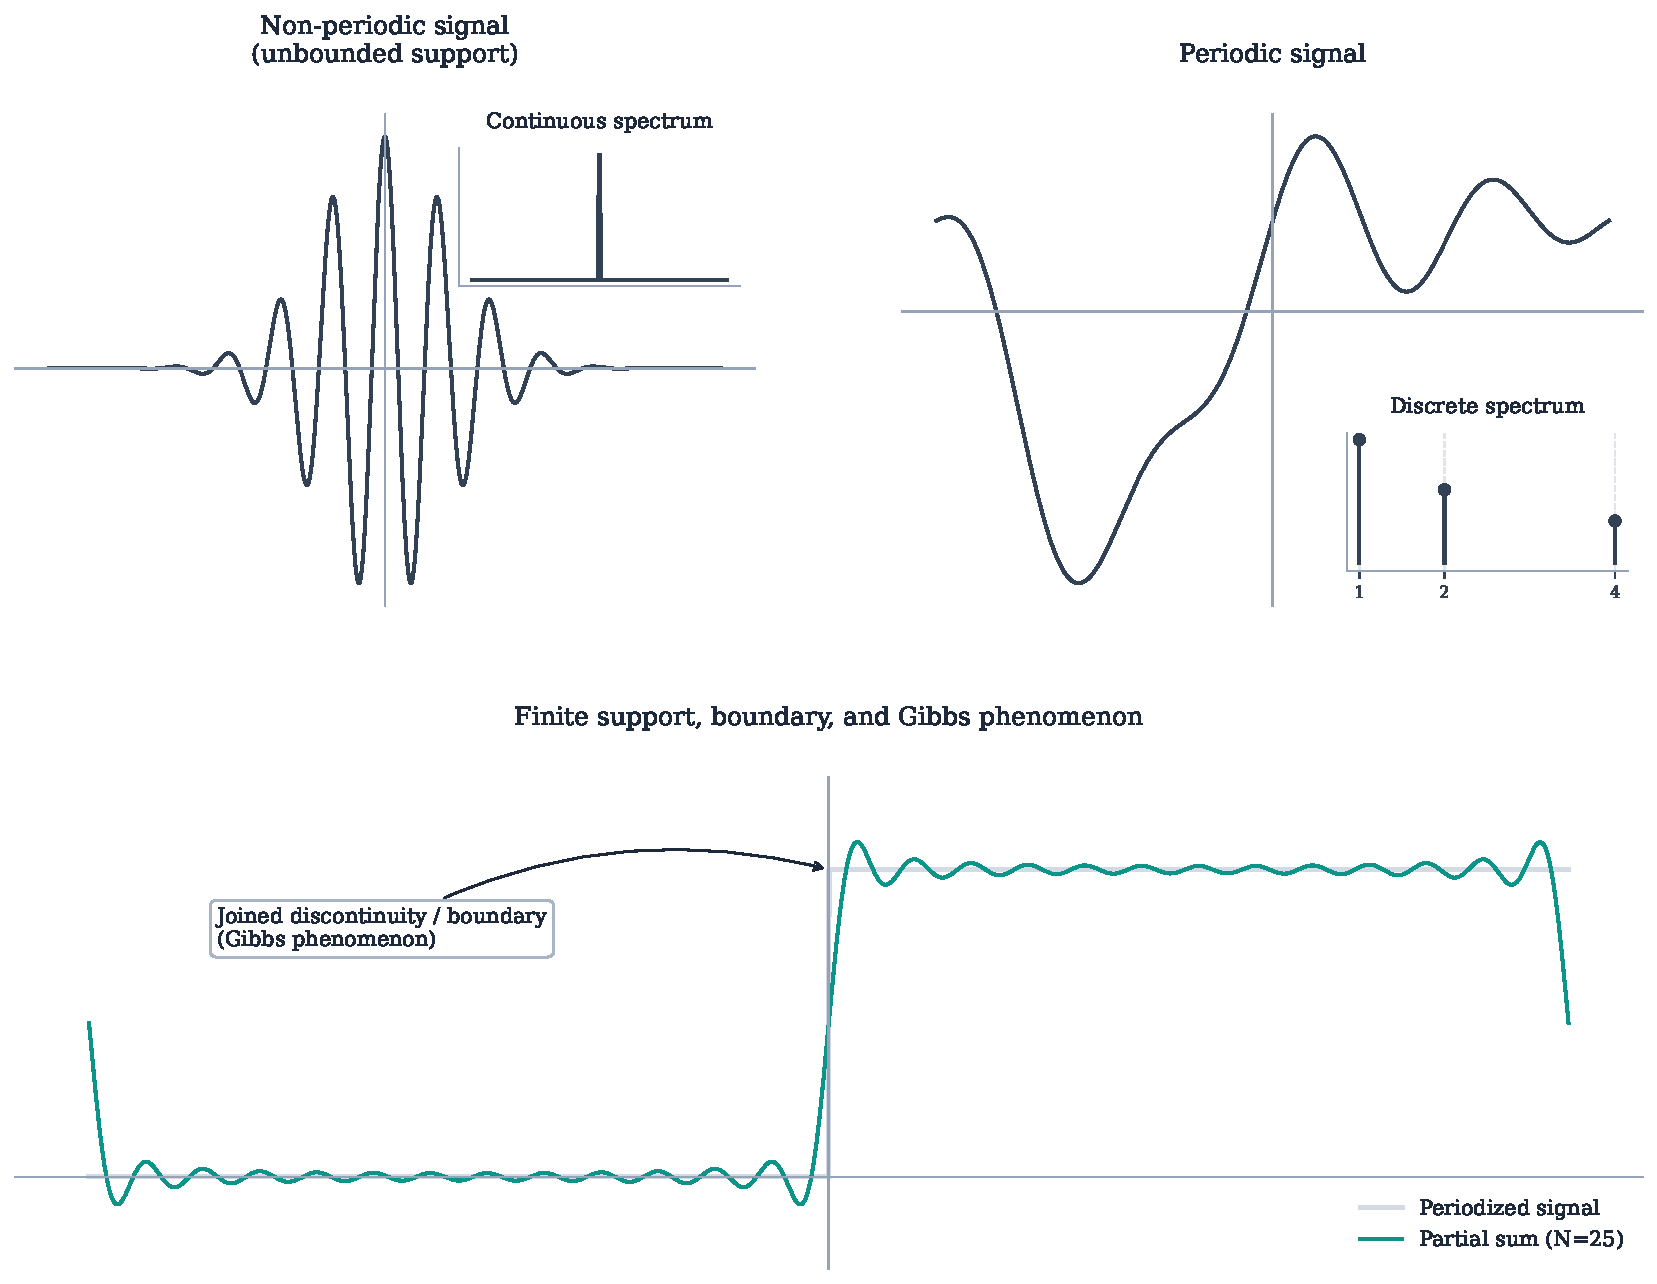
\includegraphics[width=0.8\textwidth]{figures/theory/fourier_periodicite_gibbs_en.pdf}
    \caption{Left: a nonperiodic signal defined on an infinite domain has a continuous spectrum.
    Center: a periodic signal has a discrete spectrum consisting of harmonic lines.
    Right: a signal with finite support may exhibit an artificial discontinuity when periodized.}
    \label{fig:gibbs}
\end{figure}

\section{Detailed Proof of the BCCB Structure}
\label{app:preuve_bccb}

We revisit the case of a single-channel 2D circular convolution. The goal is to show,
step by step, why the matrix $M$ associated with this convolution is block-circulant
and why each of its blocks is itself circulant.

\begin{proof}

Let $X\in\mathbb{C}^{N\times N}$ denote the input image, $Y\in\mathbb{C}^{N\times N}$ the output
image, and $h\in\mathbb{C}^{N\times N}$ the filter. Recall that, in the circular setting, 2D convolution is written as

$$\begin{aligned}
    Y[m,n] &= \sum_{a=0}^{N-1} \sum_{b=0}^{N-1} h[a,b] \, X[(m-a)\bmod N, \, (n-b)\bmod N] \\
           &= \sum_{a=0}^{N-1} \sum_{b=0}^{N-1} h[(m-a)\bmod N, \, (n-b)\bmod N] \, X[a, b].
\end{aligned}$$

With column-wise vectorization, the input entry $X[r,s]$ corresponds to the vectorized index
$r+Ns$, and the output entry $Y[m,n]$ corresponds to the vectorized index $m+Nn$. The matrix $M$ is defined
by
\[
    \operatorname{vec}(Y)=M\operatorname{vec}(X).
\]
The entry of $M$ in row $m+Nn$ and column $r+Ns$ therefore indicates how pixel
$X[r,s]$ contributes to pixel $Y[m,n]$.

According to the 2D convolution formula, this contribution is given by
\[
    M_{m+Nn,\;r+Ns}
    =
    h[(m-r)\bmod N,\,(n-s)\bmod N].
\]
This formula is central to the proof: the entry depends only on the circular
shifts between the input and output positions.

We now partition the matrix $M$ into $N\times N$ blocks, each of size $N\times N$:
\[
M =
\begin{pmatrix}
B_{0,0} & B_{0,1} & \cdots & B_{0,N-1} \\
B_{1,0} & B_{1,1} & \cdots & B_{1,N-1} \\
\vdots  & \vdots  & \ddots & \vdots \\
B_{N-1,0} & B_{N-1,1} & \cdots & B_{N-1,N-1}
\end{pmatrix}.
\]
In this partition, block $B_{n,s}$ describes the effect of column $s$ of the input image on
column $n$ of the output image.

The entries of this block are therefore
\[
    (B_{n,s})_{m,r}
    =
    M_{m+Nn,\;r+Ns}
    =
    h[(m-r)\bmod N,\,(n-s)\bmod N].
\]

Now fix two columns $n$ and $s$. Their circular shift is
\[
    \delta = (n-s)\bmod N.
\]
With this notation, the preceding expression becomes
\[
    (B_{n,s})_{m,r}
    =
    h[(m-r)\bmod N,\delta].
\]

For a fixed $\delta$, the entry $(B_{n,s})_{m,r}$ depends on $m$ and $r$ only through
the circular difference $(m-r)\bmod N$. This means that the rows of the block repeat under
circular shifts. In other words, each block $B_{n,s}$ is a circulant matrix.

To make this more explicit, define the vector
\[
h_\delta =
\begin{pmatrix}
h[0,\delta] \\
h[1,\delta] \\
\vdots \\
h[N-1,\delta]
\end{pmatrix}.
\]
Block $B_{n,s}$ is then the circulant matrix constructed from this vector:
\[
    B_{n,s}
    =
    C_{h_\delta}.
\]
Since $\delta=(n-s)\bmod N$, we can also write
\[
    B_{n,s}
    =
    C_{h_{(n-s)\bmod N}}.
\]

This formula reveals the second level of circularity. As $n$ and $s$ change,
the blocks do not vary arbitrarily: they depend only on the circular shift
$(n-s)\bmod N$. The blocks themselves are therefore arranged in a circulant pattern.

The full matrix $M$ can then be written as
\[
M =
\begin{pmatrix}
C_{h_0}     & C_{h_{N-1}} & C_{h_{N-2}} & \cdots & C_{h_1} \\
C_{h_1}     & C_{h_0}     & C_{h_{N-1}} & \cdots & C_{h_2} \\
C_{h_2}     & C_{h_1}     & C_{h_0}     & \cdots & C_{h_3} \\
\vdots      & \vdots      & \vdots      & \ddots & \vdots \\
C_{h_{N-1}} & C_{h_{N-2}} & C_{h_{N-3}} & \cdots & C_{h_0}
\end{pmatrix}.
\]

This representation clearly exhibits the two required properties:
\[
    \boxed{\text{each block is circulant}}
    \qquad\text{and}\qquad
    \boxed{\text{the blocks themselves form a circulant pattern}.}
\]
Consequently, $M$ is indeed a block-circulant matrix with circulant blocks, that is,
a BCCB matrix.

\end{proof}

\section{Detailed Proof for Skip Connections}
\label{app:preuve_skip_connection}

We revisit the identity \textit{skip connection} studied in Section~\ref{sec:skip-normalisation}.
The goal is to verify explicitly that the right singular vectors retain the same frequency structure as in the case without a \textit{skip connection}.

\begin{proof}

Let $a \in \mathbb{C}^m$ be a right singular vector of $G_{\mathrm{skip}}^{(w)}$, associated with a singular value $\sigma$ and a left singular vector $b \in \mathbb{C}^m$:
\[
G_{\mathrm{skip}}^{(w)}a = \sigma b.
\]

In the full network space, consider the vector
\[
v = a \otimes (Q_N)_w.
\]
In the same notation as before, this corresponds to
\[
v = a \otimes (F_N)_u \otimes (F_N)_v,
\]
where the flattened index $w$ corresponds to the spatial frequency pair $(u,v)$.

Now apply the operator $M_{\mathrm{skip}}$ to this vector:
\begin{align*}
M_{\mathrm{skip}}v
&=
(I_m \otimes Q_N)(L + I_{mN^2})(I_m \otimes Q_N)^H
\bigl(a \otimes (Q_N)_w\bigr).
\end{align*}

Since $(Q_N)_w = Q_N e_w$, we have
\[
a \otimes (Q_N)_w
=
(I_m \otimes Q_N)(a \otimes e_w).
\]
Thus,
\begin{align*}
M_{\mathrm{skip}}v
&=
(I_m \otimes Q_N)(L + I_{mN^2})(a \otimes e_w).
\end{align*}

The standard basis vector $e_w$ selects the coefficients associated with frequency $w$.
At this frequency, the central operator acts as the augmented mixing matrix
\[
G_{\mathrm{skip}}^{(w)} = G^{(w)} + I_m.
\]
Thus, its action on the channels separates from its action on the spatial frequency:
\begin{align*}
(L + I_{mN^2})(a \otimes e_w)
&= (G^{(w)}a + I_m a) \otimes e_w \\
&= (G_{\mathrm{skip}}^{(w)}a) \otimes e_w.
\end{align*}

Since $a$ is a right singular vector of $G_{\mathrm{skip}}^{(w)}$, we have
\[
G_{\mathrm{skip}}^{(w)}a = \sigma b.
\]
We therefore obtain
\[
(L + I_{mN^2})(a \otimes e_w) = \sigma(b \otimes e_w).
\]

Substituting this result into the expression for $M_{\mathrm{skip}}v$ gives:
\begin{align*}
M_{\mathrm{skip}}v
&=
(I_m \otimes Q_N) \bigl( \sigma(b \otimes e_w) \bigr) \\
&= \sigma \bigl( (I_m b) \otimes (Q_N e_w) \bigr) \\
&= \sigma\bigl(b \otimes (Q_N)_w\bigr).
\end{align*}

Thus, applying $M_{\mathrm{skip}}$ to the vector
\[
v = a \otimes (Q_N)_w
\]
indeed yields an output vector with the same spatial frequency:
\[
M_{\mathrm{skip}}v = \sigma\bigl(b \otimes (Q_N)_w\bigr).
\]

The spatial frequency $(Q_N)_w$ is therefore preserved. Only the overall amplitude, given by $\sigma$, and the channel profile, given by $b$, change.

Consequently, the right singular vectors of the operator with a \textit{skip connection} remain of the form
\[
a \otimes (Q_N)_w,
\]
that is,
\[
a \otimes (F_N)_u \otimes (F_N)_v.
\]
\end{proof}

\section{Graphical Representation of Stride}

\definecolor{gridblue}{HTML}{006699}
\definecolor{gridteal}{HTML}{148F77}
\definecolor{gridred}{HTML}{E74C3C}
\definecolor{selectgray}{HTML}{D3D3D3}

\begin{figure}[H]
    \centering
    \begin{tikzpicture}[scale=0.75, every node/.style={transform shape}] 

        % =========================================================================
        % GAUCHE : Stride = 1
        % =========================================================================
        \begin{scope}[shift={(0,0)}]
            % Titre parfaitement centré sur l'axe vertical de la figure (x=0)
            \node[font=\large\bfseries] at (0,6.5) {Stride = 1 (Continuous sliding)};
            
            \begin{scope}[x={(0.6cm,0.3cm)}, y={(-0.6cm,0.3cm)}, z={(0cm,0.8cm)}]
                
                % --- Image d'entrée 5x5 ---
                \fill[gridblue] (0,0,0) -- (5,0,0) -- (5,5,0) -- (0,5,0) -- cycle;
                \draw[black, thick, join=round] (0,0,0) -- (5,0,0) -- (5,5,0) -- (0,5,0) -- cycle;
                \foreach \i in {1,...,4} {
                    \draw[black, thick] (\i,0,0) -- (\i,5,0);
                    \draw[black, thick] (0,\i,0) -- (5,\i,0);
                }
                
                % --- Filtre initial ---
                \fill[gridred, opacity=0.8] (0,0,0) -- (3,0,0) -- (3,3,0) -- (0,3,0) -- cycle;
                \draw[black, thick, join=round] (0,0,0) -- (3,0,0) -- (3,3,0) -- (0,3,0) -- cycle;
                \foreach \i in {1,2} {
                    \draw[black, thick] (\i,0,0) -- (\i,3,0);
                    \draw[black, thick] (0,\i,0) -- (3,\i,0);
                }

                % --- Mouvement du filtre (Fantôme) ---
                \draw[gridred, ultra thick, dashed, opacity=1] (1,0,0) -- (4,0,0) -- (4,3,0) -- (1,3,0) -- cycle;
                
                % --- Flèche de direction unique (+1) très visible ---
                \draw[->, ultra thick, gridred, line join=round] (1.5,1.5,0) -- (2.5,1.5,0) 
                    node[midway, sloped, below, yshift=-3pt, font=\bfseries\large, fill=white, fill opacity=0.9, text opacity=1, inner sep=3pt, rounded corners=2pt] {+1};
                
                % --- Projection (Pointillés très marqués) ---
                \draw[black!70, very thick, dashed] (0,0,0) -- (1,1,4.5);
                \draw[black!70, very thick, dashed] (3,0,0) -- (2,1,4.5);
                \draw[black!70, very thick, dashed] (3,3,0) -- (2,2,4.5);
                \draw[black!70, very thick, dashed] (0,3,0) -- (1,2,4.5);
                
                % --- Image de sortie 3x3 ---
                \fill[gridteal] (1,1,4.5) -- (4,1,4.5) -- (4,4,4.5) -- (1,4,4.5) -- cycle;
                \draw[black, thick, join=round] (1,1,4.5) -- (4,1,4.5) -- (4,4,4.5) -- (1,4,4.5) -- cycle;
                \foreach \i in {2,3} {
                    \draw[black, thick] (\i,1,4.5) -- (\i,4,4.5);
                    \draw[black, thick] (1,\i,4.5) -- (4,\i,4.5);
                }
                
                \node[anchor=south east, font=\small\bfseries] at (1,4,4.7) {Output $3 \times 3$};
            
                % Pixel calculé
                \fill[selectgray, opacity=0.9] (1,1,4.5) -- (2,1,4.5) -- (2,2,4.5) -- (1,2,4.5) -- cycle;
                \draw[black, thick] (1,1,4.5) -- (2,1,4.5) -- (2,2,4.5) -- (1,2,4.5) -- cycle;
                
            \end{scope}
            
            \node[font=\small\bfseries] at (0,-1.5) {Input $5 \times 5$};
            
        \end{scope}

        % =========================================================================
        % DROITE : Stride = 2 
        % =========================================================================
        \begin{scope}[shift={(10,0)}] 
            \node[font=\large\bfseries] at (0,6.5) {Stride = 2 (Steps of 2 positions)};

            \begin{scope}[x={(0.6cm,0.3cm)}, y={(-0.6cm,0.3cm)}, z={(0cm,0.8cm)}]
                
                % --- Image d'entrée 5x5 ---
                \fill[gridblue] (0,0,0) -- (5,0,0) -- (5,5,0) -- (0,5,0) -- cycle;
                \draw[black, thick, join=round] (0,0,0) -- (5,0,0) -- (5,5,0) -- (0,5,0) -- cycle;
                \foreach \i in {1,...,4} {
                    \draw[black, thick] (\i,0,0) -- (\i,5,0);
                    \draw[black, thick] (0,\i,0) -- (5,\i,0);
                }
                
                % --- Filtre initial ---
                \fill[gridred, opacity=0.8] (0,0,0) -- (3,0,0) -- (3,3,0) -- (0,3,0) -- cycle;
                \draw[black, thick, join=round] (0,0,0) -- (3,0,0) -- (3,3,0) -- (0,3,0) -- cycle;
                \foreach \i in {1,2} {
                    \draw[black, thick] (\i,0,0) -- (\i,3,0);
                    \draw[black, thick] (0,\i,0) -- (3,\i,0);
                }

                % --- Mouvement du filtre (Fantôme) ---
                \draw[gridred, ultra thick, dashed, opacity=1] (2,0,0) -- (5,0,0) -- (5,3,0) -- (2,3,0) -- cycle;

                % --- Flèche de direction unique (+2) ---
                \draw[->, ultra thick, gridred, line join=round] (1.5,1.5,0) -- (3.5,1.5,0) 
                    node[midway, sloped, below, yshift=-3pt, font=\bfseries\large, fill=white, fill opacity=0.9, text opacity=1, inner sep=3pt, rounded corners=2pt] {+2};

                % --- Projection (Pointillés très marqués) ---
                \draw[black!70, very thick, dashed] (0,0,0) -- (1.5,1.5,4.5);
                \draw[black!70, very thick, dashed] (3,0,0) -- (2.5,1.5,4.5);
                \draw[black!70, very thick, dashed] (3,3,0) -- (2.5,2.5,4.5);
                \draw[black!70, very thick, dashed] (0,3,0) -- (1.5,2.5,4.5);
                
                % --- Image de sortie 2x2 ---
                \fill[gridteal] (1.5,1.5,4.5) -- (3.5,1.5,4.5) -- (3.5,3.5,4.5) -- (1.5,3.5,4.5) -- cycle;
                \draw[black, thick, join=round] (1.5,1.5,4.5) -- (3.5,1.5,4.5) -- (3.5,3.5,4.5) -- (1.5,3.5,4.5) -- cycle;
                \draw[black, thick] (2.5,1.5,4.5) -- (2.5,3.5,4.5);
                \draw[black, thick] (1.5,2.5,4.5) -- (3.5,2.5,4.5);
                
                \node[anchor=south east, font=\small\bfseries] at (1.5,3.5,4.7) {Output $2 \times 2$};

                % Pixel calculé
                \fill[selectgray, opacity=0.9] (1.5,1.5,4.5) -- (2.5,1.5,4.5) -- (2.5,2.5,4.5) -- (1.5,2.5,4.5) -- cycle;
                \draw[black, thick] (1.5,1.5,4.5) -- (2.5,1.5,4.5) -- (2.5,2.5,4.5) -- (1.5,2.5,4.5) -- cycle;
                
            \end{scope}
            
            \node[font=\small\bfseries] at (0,-1.5) {Input $5 \times 5$};
            
        \end{scope}

        % =========================================================================
        % LÉGENDE 
        % =========================================================================
        \node[anchor=center, draw=black!30, thick, rounded corners, fill=white, inner sep=10pt] at (5,-3.2) {
            \begin{tikzpicture}
                \fill[gridblue] (0,0) rectangle (0.5,0.5); \node[right, font=\small\bfseries] at (0.6,0.25) {Input};
                \fill[gridred, opacity=0.8] (3,0) rectangle (3.5,0.5); \node[right, font=\small\bfseries] at (3.6,0.25) {Filter};
                \fill[gridteal] (6,0) rectangle (6.5,0.5); \node[right, font=\small\bfseries] at (6.6,0.25) {Output};
                \fill[selectgray] (9,0) rectangle (9.5,0.5); \node[right, font=\small\bfseries] at (9.6,0.25) {Computed pixel};
            \end{tikzpicture}
        };

    \end{tikzpicture}
    \caption{Effect of \textit{stride} on the output spatial resolution.}
    \label{fig:stride_comparison}
\end{figure}

\section{Illustration of Average Pooling}

\begin{figure}[H]
    \centering
    \begin{tikzpicture}[scale=0.85, transform shape]
        % --- GRILLE D'ENTREE (4x4) ---
        \draw[step=1cm, gray!40, thin] (0,0) grid (4,4);
        
        % Couleurs des blocs 2x2 (Style sobre et epure)
        \fill[blue, opacity=0.08] (0,2) rectangle (2,4);
        \fill[red, opacity=0.08] (2,2) rectangle (4,4);
        \fill[green!60!black, opacity=0.08] (0,0) rectangle (2,2);
        \fill[orange, opacity=0.08] (2,0) rectangle (4,2);

        % Cadres des blocs
        \draw[blue, thick, rounded corners=1pt] (0,2) rectangle (2,4);
        \draw[red, thick, rounded corners=1pt] (2,2) rectangle (4,4);
        \draw[green!60!black, thick, rounded corners=1pt] (0,0) rectangle (2,2);
        \draw[orange, thick, rounded corners=1pt] (2,0) rectangle (4,2);

        % Valeurs d'entree (Exemple numerique simple)
        \foreach \x/\y/\v in {0.5/3.5/1, 1.5/3.5/3, 0.5/2.5/3, 1.5/2.5/5,
                              2.5/3.5/5, 3.5/3.5/7, 2.5/2.5/7, 3.5/2.5/9,
                              0.5/1.5/2, 1.5/1.5/2, 0.5/0.5/1, 1.5/0.5/3,
                              2.5/1.5/8, 3.5/1.5/6, 2.5/0.5/9, 3.5/0.5/9} {
            \node[font=\small, text=black!70] at (\x, \y) {\v};
        }

        % --- FLECHE DE TRANSITION ---
        \draw[->, >=stealth, very thick, black!60] (4.5, 2) -- node[above, font=\footnotesize, text=black] {Local average} node[below, font=\footnotesize, text=black] {\textit{Stride} $s=2$} (7, 2);

        % --- GRILLE DE SORTIE (2x2) ---
        \begin{scope}[xshift=7.5cm, yshift=1cm]
            \draw[step=1cm, gray!40, thin] (0,0) grid (2,2);
            
            % Couleurs correspondantes
            \fill[blue, opacity=0.08] (0,1) rectangle (1,2);
            \fill[red, opacity=0.08] (1,1) rectangle (2,2);
            \fill[green!60!black, opacity=0.08] (0,0) rectangle (1,1);
            \fill[orange, opacity=0.08] (1,0) rectangle (2,1);

            % Valeurs calculees (moyennes)
            \node[font=\bfseries, text=blue!80!black] at (0.5, 1.5) {3};
            \node[font=\bfseries, text=red!80!black] at (1.5, 1.5) {7};
            \node[font=\bfseries, text=green!50!black] at (0.5, 0.5) {2};
            \node[font=\bfseries, text=orange!80!black] at (1.5, 0.5) {8};
        \end{scope}

    \end{tikzpicture}
    \caption{Spatial illustration of the \textit{average pooling} operation. Each $2 \times 2$ block of pixels in the input image is replaced by its arithmetic mean, reducing the spatial resolution by a factor of $s=2$.}
    \label{fig:avg_pooling_spatial}
\end{figure}

\section{Review of the SVD and Amplification Directions}
\label{app:svd-sensibilite}

Let
\[
    M \in \mathbb{C}^{m_{\mathrm{out}}N^2 \times m_{\mathrm{in}}N^2}
\]
be the matrix representing a multichannel convolution operator. Since this matrix is not
necessarily square, we use singular value decomposition rather than standard
eigendecomposition.

The singular value decomposition of $M$ is
\[
    M = U \Sigma V^H,
\]
where $U$ and $V$ are unitary matrices, and $\Sigma$ is a rectangular diagonal matrix
containing the singular values of $M$:
\[
    \sigma_1 \geq \sigma_2 \geq \cdots \geq 0.
\]
The columns of $V$ are called the right singular vectors of $M$: they lie in the input
space. The columns of $U$ are called the left singular vectors of $M$: they lie in
the output space.

To understand why right singular vectors describe amplification directions,
consider the positive self-adjoint matrix $M^H M$. From the SVD, we obtain
\[
    M^H M
    =
    (U\Sigma V^H)^H(U\Sigma V^H).
\]
Using $(ABC)^H = C^H B^H A^H$ gives
\[
    M^H M
    =
    V\Sigma^H U^H U \Sigma V^H.
\]
Since $U$ is unitary, $U^H U = I$, so
\[
    M^H M
    =
    V\Sigma^H \Sigma V^H.
\]
The matrix $\Sigma^H\Sigma$ is diagonal and contains the squared singular values:
\[
    \Sigma^H\Sigma
    =
    \operatorname{diag}(\sigma_1^2,\sigma_2^2,\dots).
\]
Thus,
\[
    M^H M
    =
    V
    \operatorname{diag}(\sigma_1^2,\sigma_2^2,\dots)
    V^H.
\]
This shows that the right singular vectors of $M$ are precisely the eigenvectors of
$M^H M$, and that the associated eigenvalues are the squared singular values.

In particular, if $v_i$ denotes the $i$-th column of $V$, then
\[
    M^H M v_i
    =
    V D V^H v_i
    =
    V D e_i
    =
    V(\sigma_i^2 e_i)
    =
    \sigma_i^2 v_i,
\]
where
\[
    D=\operatorname{diag}(\sigma_1^2,\sigma_2^2,\dots).
\]
Thus,
\[
    M^H M v_i = \sigma_i^2 v_i.
\]

Equivalently, the singular value $\sigma_i$ measures the amplification induced by $M$
in direction $v_i$. Indeed,
\[
    \|Mv_i\|_2^2
    =
    (Mv_i)^H(Mv_i)
    =
    v_i^H M^H M v_i
    =
    v_i^H(\sigma_i^2 v_i)
    =
    \sigma_i^2 \|v_i\|_2^2.
\]
Since $V$ is unitary, its columns form an orthonormal basis. In particular,
\[
    \|v_i\|_2 = 1.
\]
We therefore obtain
\[
    \|Mv_i\|_2 = \sigma_i.
\]

The largest singular value describes the maximum amplification of $M$ among inputs with norm
$1$:
\[
    \sigma_1
    =
    \max_{\|x\|_2=1}\|Mx\|_2.
\]
If $\sigma_1$ is simple, the direction achieving this maximum amplification is the right singular
vector $v_1$. If $\sigma_1$ has multiplicity greater than one, there is no single maximizing direction: every
unit-norm direction in the subspace associated with $\sigma_1$ yields the same amplification.

In the frequency analysis of convolutions, the network's highly sensitive directions
therefore correspond to right singular vectors associated with large singular values.

\section{Mean Fourier Spectrum of Clean Images}
\label{annexe:spectres_moyens_cifar}

This appendix presents the mean Fourier spectrum of unperturbed CIFAR-10 and CIFAR-100 images.
The aim is not to measure model sensitivity directly, but to observe which frequencies
are naturally present in the input data.

\begin{figure}[H]
    \centering
    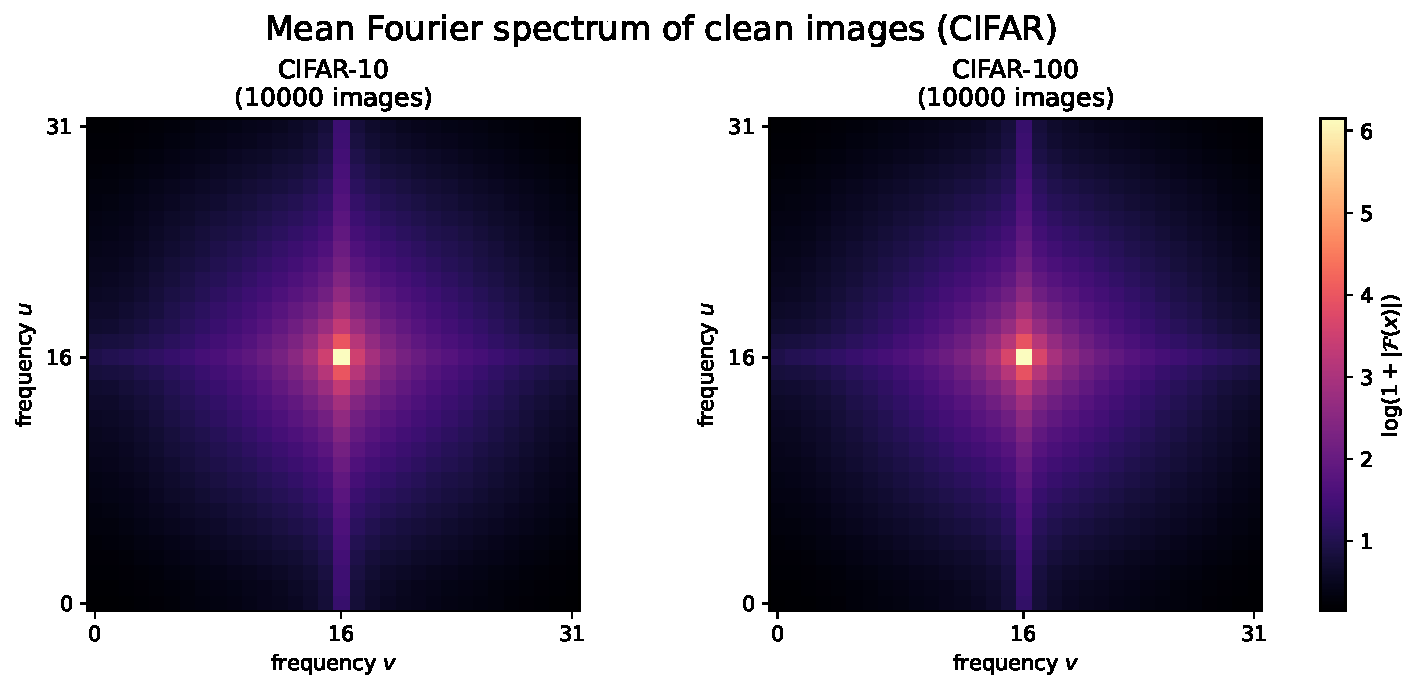
\includegraphics[width=\textwidth]{figures/results/mean_clean_spectrum_comparison_cifar_en.pdf}
    \caption{Mean Fourier spectrum of unperturbed CIFAR-10 and CIFAR-100 images. The displayed values
    correspond to $\log(1+|\mathcal{F}(x)|)$, averaged over the images in the dataset.}
    \label{fig:mean_clean_spectrum_comparison_cifar}
\end{figure}

The two datasets exhibit very similar frequency structures:
energy is strongly concentrated around the center of the spectrum and gradually decreases in an approximately
diamond-shaped pattern. The more pronounced horizontal and vertical lines also indicate that certain
frequency directions are more prevalent than others in the unperturbed images.

This observation suggests a possible interpretation of the SFA heatmaps. It shows that the input
images themselves have a nonuniform frequency organization. Model sensitivity
may therefore depend both on the architecture and on the statistics of the data used during
training.

However, this comparison remains descriptive. The mean spectrum characterizes the input images,
whereas the SFA heatmaps measure the model's response to imposed perturbations. The two should
therefore not be conflated.

\section{Supplementary Analysis: The Role of Channel Mixing in SFA}
\label{annexe:color_sfa}

In the theoretical framework presented in the previous chapter, the singular directions of a
linearized convolutional model can be written in the form
\[
    v = a \otimes q_{u,v},
\]
where \(q_{u,v}\) represents a spatial Fourier component and
\(a \in \mathbb{R}^3\) describes the mixing of the red, green, and blue channels.

The \textit{Single Fourier Attack} used in the main protocol simplifies this framework. It does not seek
to optimize the spatial frequency and the color vector \(a\) simultaneously. The same Fourier
pattern is applied to all three RGB channels, which amounts to using the vector
\[
    a_{\mathrm{uni}} = (1,1,1).
\]
The search space is therefore reduced to the choice of frequency $(u,v)$. This simplification
makes the attack much easier to evaluate, since we need only iterate over the frequencies in the
Fourier domain. It is also consistent with the $\ell_\infty$ constraint used in
the main protocol: the pattern is applied at the maximum allowed amplitude to each of the
three channels.

We then distinguish two ways of constraining channel mixing. The first
retains an $\ell_\infty$-norm constraint comparable to standard SFA, to test whether
another choice of color direction can improve the attack at the same maximum amplitude. The
second uses an $\ell_1$-type budget on the color vector's coefficients. In this case,
a vector such as $a=(3,0,0)$ is possible: the total budget is concentrated in a single channel,
which no longer corresponds exactly to the standard SFA constraint. The two variants
therefore do not measure exactly the same thing; rather, they test whether the choice of RGB
mixing can strengthen the effect of a Fourier frequency.

\subsection*{Searching for RGB Vectors at Each Frequency}

Figure~\ref{fig:color_sfa_foolratio_and_activation_grids} compares standard SFA with variants
in which the RGB vector \(a\) is chosen from a limited set of possible combinations.

\begin{figure}[H]
    \centering
    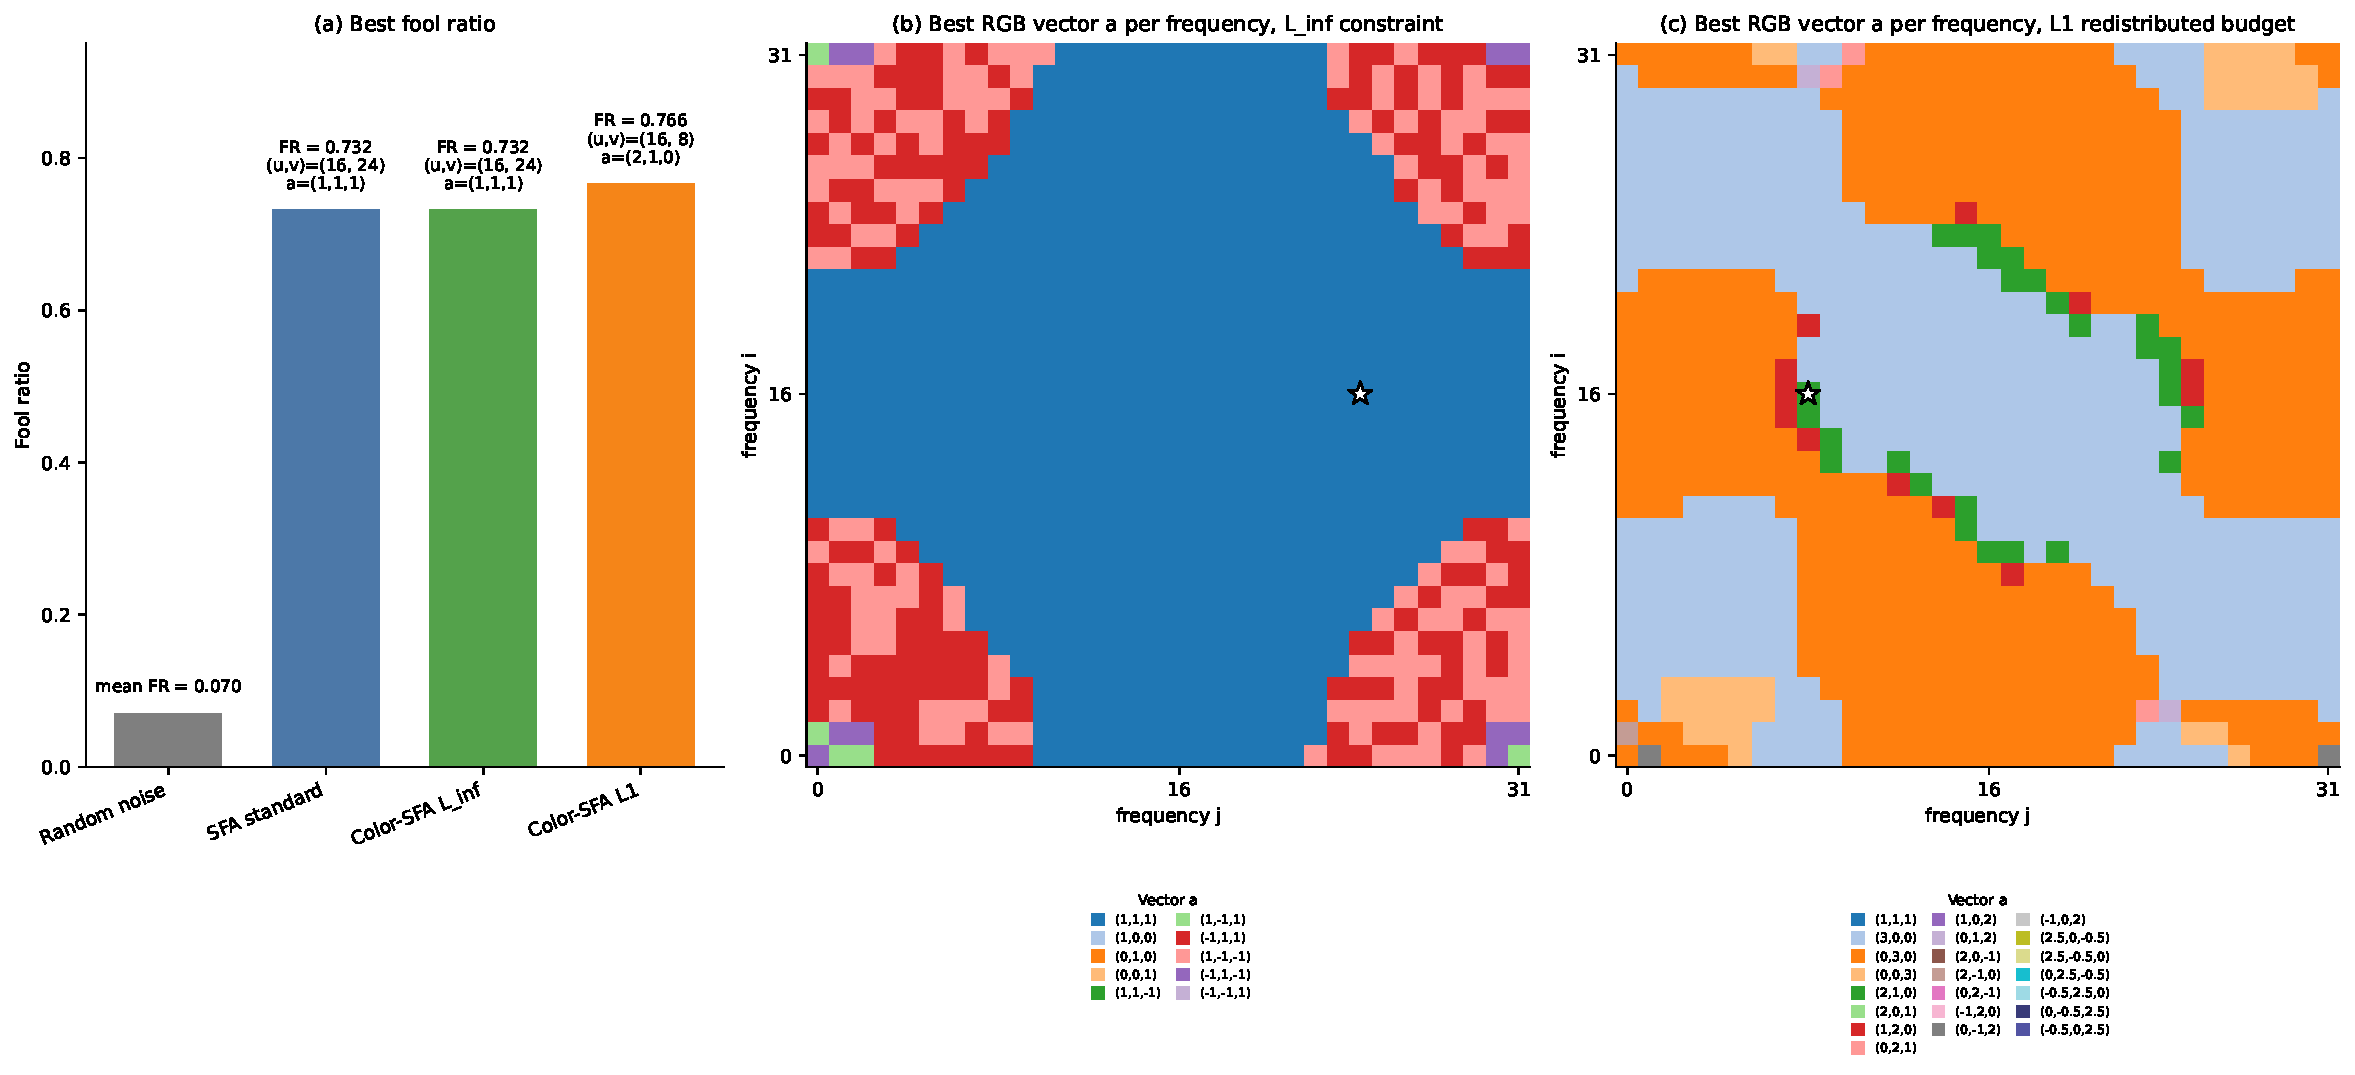
\includegraphics[width=\textwidth]{figures/results/color_sfa_foolratio_and_activation_grids.pdf}
    \caption{Comparison between standard SFA and variants in which the RGB vector \(a\) is chosen for each frequency.
    Left: the best \textit{fool ratio} obtained by each method is compared with the random-noise
    baseline. Center and right: each cell indicates the best RGB vector found for the corresponding
    frequency under two different budget constraints.}
    \label{fig:color_sfa_foolratio_and_activation_grids}
\end{figure}

In the variant renormalized in the $\ell_\infty$ norm, the best color variant achieves
almost the same result as standard SFA. This indicates that, under this constraint,
choosing a different RGB mixture does not significantly improve the attack compared with the
uniform direction $(1,1,1)$.

With the variant using an $\ell_1$ budget on the color coefficients, the best score increases slightly,
from approximately \(0.732\) to \(0.766\), with frequency \((16,8)\) and vector \(a=(2,1,0)\).
This improvement is fairly modest in our case.

\subsection*{Comparison of Fixed Color Directions}

We then compared several simple color directions:
\[
(1,1,1), \quad (1,0,0), \quad (0,1,0), \quad (0,0,1),
\]
as well as opponent color directions:
\[
(1,-1,0), \quad (1,0,-1), \quad (0,1,-1),
\]
and a luminance-like direction.

The results in Figure~\ref{fig:color_sfa_cifar10} show that the standard direction
$(1,1,1)$ remains by far the most effective. Directions applied to a single channel have a
weaker effect, while the opponent color directions $(1,-1,0)$, $(1,0,-1)$, and
$(0,1,-1)$ yield almost zero fool ratios.

\begin{figure}[H]
    \centering
    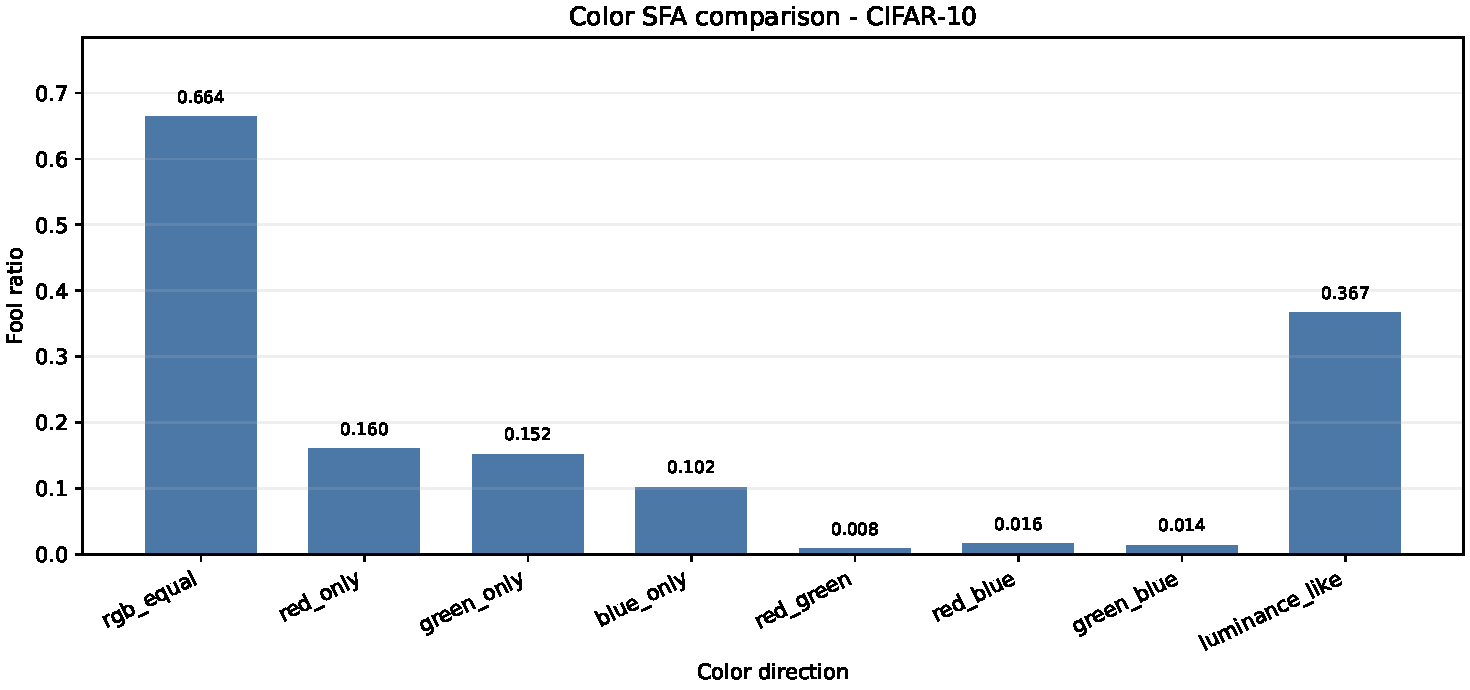
\includegraphics[width=0.85\textwidth]{figures/results/color_sfa_cifar10_barplot.pdf}
    \caption{Comparison of several color directions for the \textit{Single Fourier Attack}
    on CIFAR-10.}
    \label{fig:color_sfa_cifar10}
\end{figure}

This observation suggests that, for the frequency studied, opponent color directions
are weakly transmitted by the network. We can interpret this using the multichannel
framework. For a fixed frequency $(u,v)$, the effect of a color direction
$a \in \mathbb{R}^3$ is described by the mixing matrix $G^{(u,v)}$:
\[
    \beta = G^{(u,v)}a.
\]
Standard SFA corresponds to the choice
\[
    a_{\mathrm{uni}} = (1,1,1),
\]
that is, a common variation in all three RGB channels.

\paragraph{Ideally symmetric case.}
Suppose that, at the frequency considered, the network responds identically to the three
input channels. This amounts to assuming that the three columns of $G^{(u,v)}$ are identical:
\[
    G^{(u,v)}
    =
    \begin{pmatrix}
    | & | & | \\
    g & g & g \\
    | & | & |
    \end{pmatrix}
    =
    g
    \begin{pmatrix}
    1 & 1 & 1
    \end{pmatrix},
\]
where $g \in \mathbb{C}^{m_{\mathrm{out}}}$ describes the network's common frequency response.

Then, for any color direction $a=(a_R,a_G,a_B)$, we obtain
\[
    G^{(u,v)}a
    =
    g(a_R+a_G+a_B).
\]
Amplification therefore depends only on the sum of the components of $a$. Under an
$\ell_\infty$ constraint comparable to that of standard SFA,
\[
    |a_R|, |a_G|, |a_B| \leq 1,
\]
the absolute value of this sum is maximized by
\[
    a=(1,1,1)
\]
or its negative. Thus, in this simplified symmetric setting, the uniform direction
$a_{\mathrm{uni}}$ is optimal.

Conversely, any color direction satisfying
\[
    a_R+a_G+a_B=0
\]
is annihilated by $G^{(u,v)}$. This is the case for the opponent color directions
\[
    (1,-1,0), \qquad (1,0,-1), \qquad (0,1,-1).
\]
In this simplified model, these directions therefore belong to the kernel of the per-frequency
mixing matrix:
\[
    G^{(u,v)}a = 0.
\]

\paragraph{Approximately symmetric case.}
In a real network, the columns of $G^{(u,v)}$ are not exactly identical. However, we can
separate a component common to all three channels from a residual term:
\[
    G^{(u,v)}
    =
    g
    \begin{pmatrix}
    1 & 1 & 1
    \end{pmatrix}
    + E,
\]
where we can take
\[
    g
    =
    \frac{1}{3}G^{(u,v)}
    \begin{pmatrix}
    1 \\ 1 \\ 1
    \end{pmatrix}.
\]
The term $E$ then measures the deviation from a response that is perfectly shared by all three channels.

For an opponent color direction such that $a_R+a_G+a_B=0$, the common component
vanishes:
\[
    G^{(u,v)}a = Ea.
\]
Thus, if $\|E\|$ is small, then
\[
    \|G^{(u,v)}a\|_2
    \leq
    \|E\|\,\|a\|_2.
\]
Opponent color directions are therefore no longer exactly annihilated, but they remain
weakly transmitted when frequency-dependent channel mixing is close to a common
response.

This proposition provides a theoretical interpretation of the results observed in
Figure~\ref{fig:color_sfa_cifar10}. The high effectiveness of $(1,1,1)$ suggests that the frequency
studied primarily activates a direction common to the channels, while the low scores
of opponent color directions may be explained by near cancellation in
frequency-dependent channel mixing.

\section{Internal Heatmaps by Layer}
\label{annexe:heatmaps_internes_couches}

To complement the amplification analysis presented in the main chapter, we visualize here
the effect of Fourier perturbations at different internal levels of the network. For each frequency,
we measure the normalized mean change in activations after perturbation and then
compare it with the final \textit{fool ratio}.

\begin{figure}[H]
    \centering
    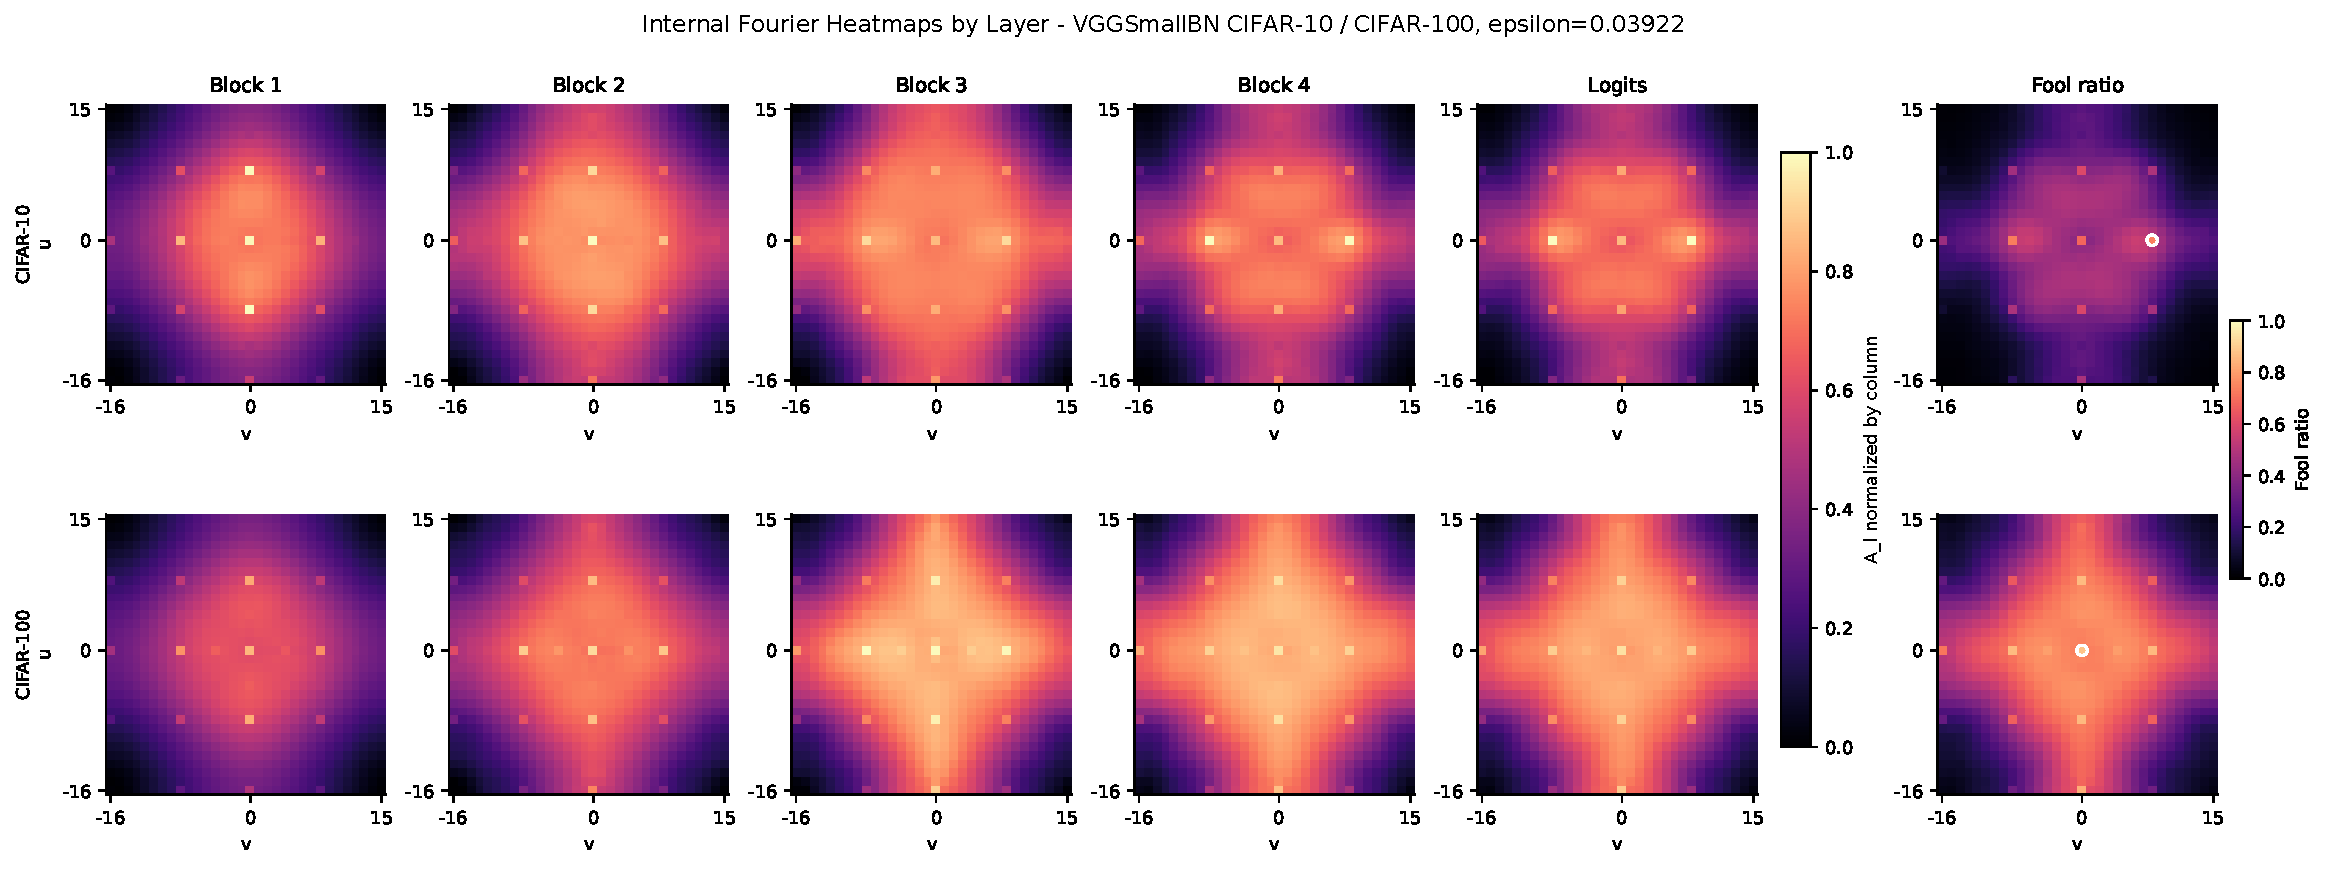
\includegraphics[width=\textwidth]{figures/results/layerwise_fourier_heatmaps_comparison_vgg_cifar10_cifar100_en.pdf}
    \caption{Internal heatmaps by layer for \texttt{VGGSmallBN} on CIFAR-10 and CIFAR-100.
    The first columns show the normalized mean change in internal activations after
    Fourier perturbation. The last column shows the final \textit{fool ratio}.}
    \label{fig:annexe_layerwise_fourier_heatmaps}
\end{figure}

These visualizations show that the frequency structure observed in the final heatmaps is
already present in the network's internal representations. It becomes more pronounced in deeper blocks and
in the logits, suggesting that certain frequencies are progressively amplified during
convolutional processing.

\section{Further Analysis of Logit Margins and Local Boundaries}
\label{annexe:marges-logits}

This appendix complements the experimental analysis in Chapter~4. The goal is to better understand
why the model trained on CIFAR-100 appears more fragile than the one trained on CIFAR-10.

\subsection{Distribution of Logit Margins}

For each image in the test set, we compute the logits produced by the model. Let
$z_{(1)}$ denote the largest logit and $z_{(2)}$ the second-largest logit. The logit margin is defined as
\[
    m(x) = z_{(1)}(x) - z_{(2)}(x).
\]

This quantity simply measures the gap between the predicted class and its closest competing class according to
the model.

Figure~\ref{fig:logit-margin-histograms} compares the distributions of logit margins for
VGGSmallBN on CIFAR-10 and CIFAR-100. The CIFAR-100 distribution is
much more concentrated at small margins. The median is approximately $4.15$ for CIFAR-100,
compared with approximately $11.12$ for CIFAR-10. This means that, on CIFAR-100, the model's predictions
are, on average, less strongly separated from their second-best class.

\begin{figure}[H]
    \centering
    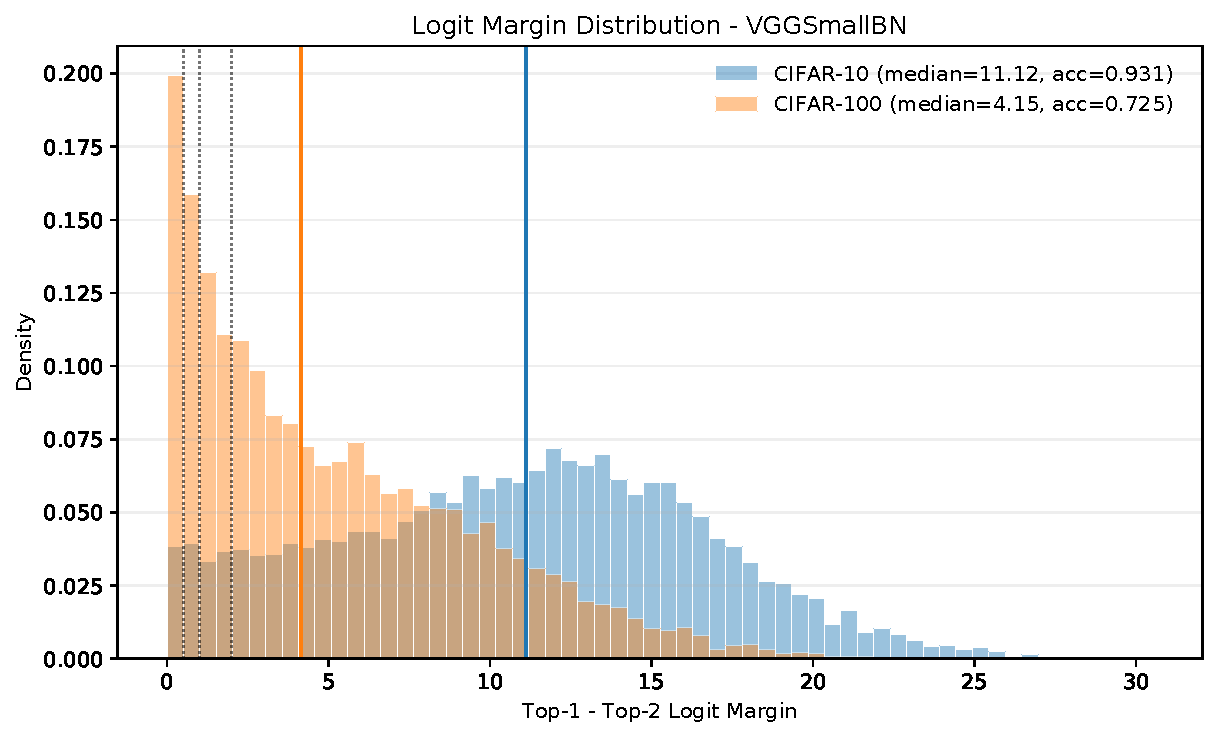
\includegraphics[width=0.85\textwidth]{figures/results/logit_margin_histograms_cifar10_cifar100_en.pdf}
    \caption{Distribution of logit margins for VGGSmallBN on CIFAR-10 and CIFAR-100. The margin is defined as the difference between the largest and second-largest logits.}
    \label{fig:logit-margin-histograms}
\end{figure}

This result provides further support for the interpretation proposed in Chapter~4:
the greater fragility observed on CIFAR-100 arises not only from the choice of a particular
frequency, but also from the apparently weaker separation between the model's decisions.

% \subsection{Carte moyenne de stabilité locale}

% En complément de l'analyse des marges logits, nous construisons une carte moyenne de stabilité
% locale autour des images correctement classées. L'objectif est de visualiser, dans une coupe
% bidimensionnelle de l'espace d'entrée, dans quelle mesure les prédictions restent stables lorsque
% l'on perturbe les images selon deux directions fréquentielles sensibles.

% Pour une image $x$, on considère les perturbations de la forme
% \[
%     x_{\alpha,\beta}
%     =
%     x + \alpha d_1 + \beta d_2,
% \]
% où $d_1$ correspond à la direction SFA principale du dataset, et $d_2$ à une seconde direction
% fréquentielle sensible.

% Pour chaque point $(\alpha,\beta)$ de la grille, nous calculons la proportion d'images pour
% lesquelles la prédiction reste identique à celle de l'image propre :
% \[
%     P_{\mathrm{same}}(\alpha,\beta)
%     =
%     \frac{1}{M}
%     \sum_{k=1}^{M}
%     \mathbf{1}\left[
%         f(x_k+\alpha d_1+\beta d_2)=f(x_k)
%     \right].
% \]
% Cette quantité vaut $1$ lorsque toutes les images gardent la même prédiction, et $0$ lorsque
% toutes les prédictions changent. Elle fournit donc une mesure moyenne de la stabilité locale du
% modèle dans la coupe considérée.

% Les cartes sont calculées sur $500$ images correctement classées par dataset, avec une grille
% de taille $41\times 41$.

% \begin{figure}[H]
%     \centering
%     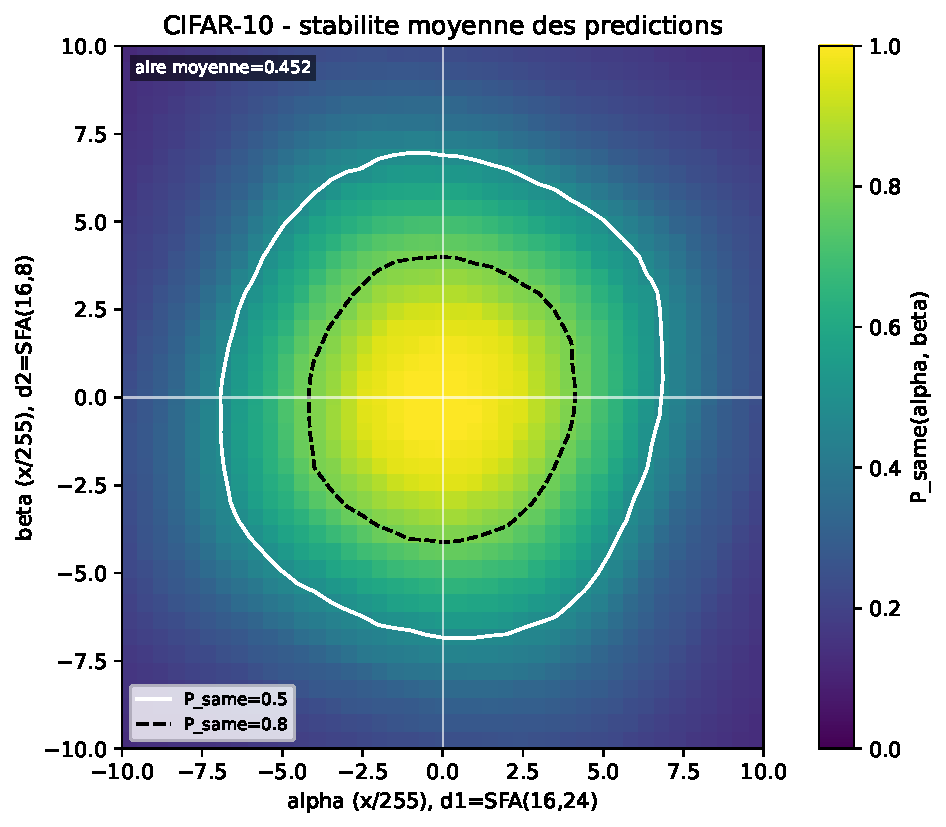
\includegraphics[width=0.48\textwidth]{figures/results/average_decision_boundary_cifar10.pdf}
%     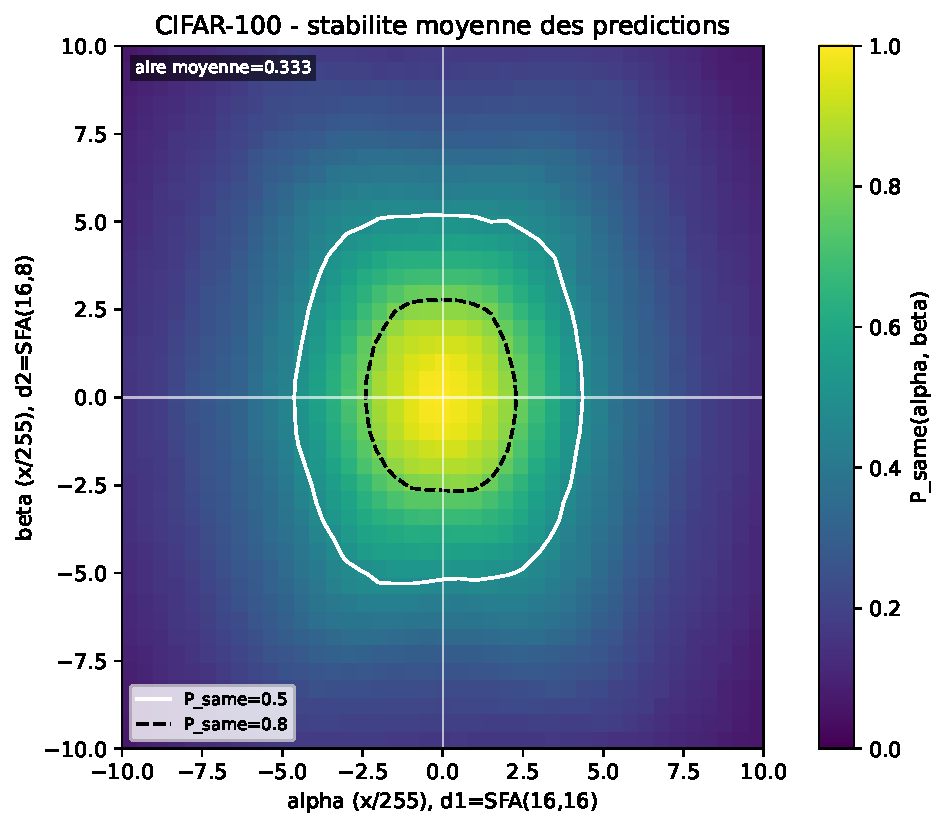
\includegraphics[width=0.48\textwidth]{figures/results/average_decision_boundary_cifar100.pdf}
%     \caption{Cartes moyennes de stabilité locale pour VGGSmallBN sur CIFAR-10 et CIFAR-100. Chaque point indique la proportion d'images dont la prédiction reste inchangée après perturbation selon deux directions fréquentielles sensibles.}
%     \label{fig:average-decision-boundary}
% \end{figure}

% \begin{table}[H]
%     \centering
%     \begin{tabular}{lcccc}
%         \toprule
%         Dataset & Aire stable moyenne & Largeur $P_{\mathrm{same}}\geq 0.5$ & Largeur $P_{\mathrm{same}}\geq 0.8$ & $\alpha$ critique moyen \\
%         \midrule
%         CIFAR-10  & 0.4518 & $13.00/255$ & $8.00/255$ & $5.81/255$ \\
%         CIFAR-100 & 0.3330 & $8.50/255$  & $4.00/255$ & $4.46/255$ \\
%         \bottomrule
%     \end{tabular}
%     \caption{ Les largeurs sont mesurées sur la ligne $\beta=0$, avec Les coefficients $\alpha$ et 
%     $\beta$ qui varient dans l'intervalle $[-10/255,10/255]$}
%     \label{tab:average-decision-boundary}
% \end{table}

% Les résultats du tableau~\ref{tab:average-decision-boundary} montrent que la région moyenne de
% stabilité est plus réduite sur CIFAR-100 que sur CIFAR-10. L'aire stable moyenne passe de
% $0.4518$ à $0.3330$, et la largeur de la région stable le long de la direction SFA diminue également.
% Pour le seuil $P_{\mathrm{same}}\geq 0.8$, cette largeur est divisée par deux, passant de $8.00/255$
% sur CIFAR-10 à $4.00/255$ sur CIFAR-100.

% Cette observation est cohérente avec les résultats principaux du chapitre~4 : le modèle entraîné
% sur CIFAR-100 est globalement plus sensible aux perturbations fréquentielles. Elle complète
% également l'analyse des marges logits, en montrant que cette fragilité se manifeste aussi dans
% une coupe locale de l'espace d'entrée.

% Il faut toutefois rester prudent dans l'interprétation. Ces cartes ne représentent pas la frontière
% de décision complète du réseau, qui vit dans un espace de dimension $32\times32\times3$.
% Elles décrivent seulement une coupe bidimensionnelle construite à partir de deux directions
% fréquentielles sensibles. Elles doivent donc être lues comme une visualisation complémentaire,
% et non comme une preuve complète de la géométrie globale des frontières de décision.


\bibliographystyle{plain}
\bibliography{formalisme/references}

\end{document}
